%==============================================================================
%  Simulation-Based Decision Support for Warehouse Workforce Planning and
%  Order Sequencing under Differentiated Service-Level Constraints
%
%  Master's Thesis - International Master in Industrial Management (IMIM)
%  Author: Ignacio Gonzalez
%
%  Compile with:  latexmk -pdf main.tex
%  (or: pdflatex -> bibtex -> pdflatex -> pdflatex)
%==============================================================================
\documentclass[11pt,a4paper,oneside]{report}

%------------------------------------------------------------------ encoding --
\usepackage[utf8]{inputenc}
\usepackage[T1]{fontenc}
% Latin Modern: scalable Type1 outlines. Required for microtype font expansion,
% which cannot work with the bitmap (pk) versions of the default Computer Modern.
\usepackage{lmodern}
\usepackage[british]{babel}
\usepackage{csquotes}

%--------------------------------------------------------------------- maths --
\usepackage{amsmath}
\usepackage{amssymb}
\usepackage{siunitx}
\sisetup{group-separator={,},group-minimum-digits=4,detect-weight=true}

%-------------------------------------------------------------------- layout --
\usepackage[a4paper,top=2.7cm,bottom=2.7cm,left=3.0cm,right=2.5cm]{geometry}
\usepackage{microtype}
\usepackage{setspace}
\onehalfspacing
\usepackage{emptypage}

%------------------------------------------------------------------ graphics --
\usepackage{graphicx}
\graphicspath{{figures/}}
\usepackage{caption}
\usepackage{subcaption}
\captionsetup{font=small,labelfont=bf,width=0.94\textwidth}

%--------------------------------------------------------------------- tikz ----
\usepackage{tikz}
\usetikzlibrary{arrows.meta,positioning,shapes.geometric,fit,backgrounds,calc}
% Shared diagram styles, so every conceptual figure in the thesis reads as one family.
\tikzset{
  stage/.style   = {draw=thesisblue, fill=thesisblue!8, rounded corners=2pt,
                    minimum width=2.1cm, minimum height=0.95cm, align=center,
                    font=\small\bfseries, thick},
  queue/.style   = {draw=black!45, fill=black!4, minimum width=0.85cm,
                    minimum height=0.95cm, align=center, font=\scriptsize},
  block/.style   = {draw=black!55, fill=white, rounded corners=2pt,
                    minimum width=6.4cm, minimum height=0.82cm, align=center,
                    font=\small},
  entry/.style   = {draw=thesisblue, fill=thesisblue!12, rounded corners=2pt,
                    minimum width=4.5cm, minimum height=0.9cm, align=center,
                    font=\small\bfseries},
  endnode/.style     = {draw=black!70, fill=black!6, rounded corners=2pt,
                    minimum width=6.4cm, minimum height=0.9cm, align=center,
                    font=\small\bfseries},
  flow/.style    = {-{Stealth[length=2.2mm]}, thick, draw=black!70},
  note/.style    = {font=\scriptsize\itshape, text=black!60, align=center},
}

%-------------------------------------------------------------------- tables --
\usepackage{booktabs}
\usepackage{longtable}
\usepackage{tabularx}
\usepackage{array}
\usepackage{multirow}
\newcolumntype{L}[1]{>{\raggedright\arraybackslash}p{#1}}
\newcolumntype{C}[1]{>{\centering\arraybackslash}p{#1}}
\newcolumntype{R}[1]{>{\raggedleft\arraybackslash}p{#1}}
\renewcommand{\arraystretch}{1.15}

%---------------------------------------------------------------- references --
\usepackage[round,authoryear]{natbib}
\bibliographystyle{apalike}
\setlength{\bibsep}{4pt}
% The manual asks for a "List of References"; the report class defaults to "Bibliography".
% babel resets \bibname at \begin{document}, so the change must be hooked into the
% language's caption list rather than applied directly.
\addto\captionsbritish{\renewcommand{\bibname}{References}}

%--------------------------------------------------------------- hyperlinks ---
\usepackage[hidelinks,breaklinks=true]{hyperref}
\usepackage[capitalise,nameinlink]{cleveref}

%-------------------------------------------------------------------- extras --
\usepackage{enumitem}
\setlist{itemsep=2pt,parsep=0pt,topsep=4pt}
\usepackage{fancyhdr}
\usepackage{titlesec}
\usepackage{xcolor}
\definecolor{thesisblue}{HTML}{1F3A5F}

\titleformat{\chapter}[display]
  {\normalfont\Large\bfseries\color{thesisblue}}
  {\chaptertitlename\ \thechapter}{12pt}{\LARGE}
\titlespacing*{\chapter}{0pt}{-18pt}{26pt}

\pagestyle{fancy}
\fancyhf{}
\fancyhead[L]{\small\nouppercase{\leftmark}}
\fancyhead[R]{\small\thepage}
\renewcommand{\headrulewidth}{0.4pt}
\fancypagestyle{plain}{\fancyhf{}\fancyfoot[C]{\small\thepage}
  \renewcommand{\headrulewidth}{0pt}}

% Convenience macros -----------------------------------------------------------
\newcommand{\rgm}[1]{\texttt{#1}}                 % workforce regime label
\newcommand{\policy}[1]{\textsc{#1}}              % policy name
% Monetary amounts. The economic parameters are scenario assumptions expressed in euros;
% \eur{74085} renders as EUR 74,085 with a thin space and thousands separators.
\newcommand{\eur}[1]{\text{EUR}\,\num{#1}}
\newcommand{\code}[1]{\texttt{\small #1}}

\begin{document}

%==============================================================================
%  FRONT MATTER
%==============================================================================
\pagenumbering{roman}

%==============================================================================
%  TITLE PAGE
%
%  NOTE FOR OVERLEAF: this file is deliberately self-contained. If you have the
%  official IMIM cover page (with the imim / UPM / Heriot-Watt logos), replace
%  the ENTIRE contents of this file with it -- nothing else in the project
%  depends on anything defined here.
%
%  Two placeholders remain to be filled in before submission:
%    TODO_TUTOR_FULL_NAME
%    TODO_SUBMISSION_MONTH_YEAR
%==============================================================================
\begin{titlepage}
\thispagestyle{empty}
\centering
\vspace*{1.6cm}

{\scshape\large International Master in Industrial Management\par}
\vspace{0.3cm}
{\small Universidad Polit\'ecnica de Madrid \quad$\cdot$\quad Heriot-Watt University\par}
\vspace{0.2cm}
{\small Edition 2025--2027\par}

\vspace{2.2cm}
\rule{\textwidth}{0.6pt}
\vspace{0.7cm}

{\LARGE\bfseries
Simulation-Based Decision Support for

\vspace{0.25em}
Warehouse Workforce Planning and Order Sequencing

\vspace{0.25em}
under Differentiated Service-Level Constraints\par}

\vspace{0.7cm}
\rule{\textwidth}{0.6pt}

\vspace{2.4cm}
{\large\textbf{Master's Thesis}\par}

\vspace{1.6cm}
{\large Author:\par}
\vspace{0.2cm}
{\Large Ignacio Gonz\'alez\par}

\vspace{1.2cm}
{\large Master's Thesis Tutor:\par}
\vspace{0.2cm}
{\Large TODO\_TUTOR\_FULL\_NAME\par}

\vfill
{\large TODO\_SUBMISSION\_MONTH\_YEAR\par}
\vspace{1.2cm}
\end{titlepage}

\cleardoublepage

\chapter*{Acknowledgements}
\addcontentsline{toc}{chapter}{Acknowledgements}
\markboth{Acknowledgements}{Acknowledgements}

I would like to thank my thesis tutor for the guidance and the critical questions that shaped
this work, and the teaching staff of the International Master in Industrial Management for the
methodological grounding that made it possible to approach an operational problem as a research
question rather than only as an engineering exercise.

I am also grateful to the colleagues I worked with during my summer internship at Baobab
Soluciones. The conversations there about optimisation and decision-support applications in
industry are what first made me curious about how these techniques behave in warehouse
operations, and that curiosity became the starting point of this thesis.

Finally, I would like to thank my family and friends for their patience and encouragement
throughout the months this project took.

\chapter*{Conflict of Interest Statement}
\addcontentsline{toc}{chapter}{Conflict of Interest Statement}
\markboth{Conflict of Interest Statement}{Conflict of Interest Statement}

The subject of this thesis was motivated by discussions held during a summer internship at
Baobab Soluciones, where questions around optimisation and decision-support applications in
industrial settings prompted my interest in applying related techniques to warehouse
operations. The research reported here was subsequently developed as an independent academic
project.

The company did not commission, fund, supervise or review this work, and does not endorse its
results. No proprietary, confidential or client data were used at any point: all experiments
reported in this thesis were carried out on synthetic data generated specifically for the
study, as described in \Cref{sec:data-provenance}. The warehouse modelled here is a
generic three-stage fulfilment operation and does not represent any real or named organisation.

The author declares no financial or personal conflict of interest in relation to this work.

\chapter*{Extended Abstract}
\addcontentsline{toc}{chapter}{Extended Abstract}
\markboth{Extended Abstract}{Extended Abstract}

\section*{Context and objective}

Warehouses serving e-commerce demand face a monthly planning decision with two components that
are usually treated separately: how much labour capacity to assign to each stage of the
fulfilment process, and in what order to release the work that queues at those stages. Capacity
is typically sized from aggregate workload ratios, while the sequencing rule is treated as a
fixed operating condition. Two features of modern fulfilment make that separation
unsatisfactory. Demand is bursty and seasonal, so queueing effects that aggregate ratios cannot
represent determine whether a plan actually holds. And service commitments are differentiated:
urgent and normal orders carry very different deadlines, so a single aggregate service figure
can conceal complete failure of the more demanding class.

The objective of this thesis is to design, implement and evaluate a simulation-based
decision-support framework that recommends a monthly workforce configuration and an order
sequencing policy jointly, under class-specific service constraints and an explicit economic
objective, and that explains its recommendations well enough to be acted on.

\section*{Theoretical background}

The work draws on four bodies of literature. Warehouse operations research establishes order
picking as the dominant component of warehouse operating cost. Queueing theory explains why
capacity sized to average requirements does not deliver average performance, since waiting grows
non-linearly with utilisation. Scheduling research establishes that rules using due-date
information outperform first-in-first-out under congestion, while priority queueing establishes
that a non-pre-emptive priority discipline redistributes waiting between classes rather than
removing it. Reinforcement learning provides a means of deriving a sequencing policy from
experience rather than specifying one in advance.

The position this thesis occupies is one of integration rather than novelty in any single
component. Existing work generally treats capacity and sequencing as separate problems and
evaluates sequencing rules against aggregate objectives; this study treats them as one joint
decision evaluated against a conjunction of class-specific constraints.

\section*{Methodology}

A discrete-event simulation model represents a three-stage fulfilment process --- picking,
packing and dispatch --- each with its own queue and dedicated worker pool. Orders are
heterogeneous, and critically their workload is stage-differentiated: product family,
complexity and urgency multiply an order's workload differently at each stage, so a fragile
order is slightly harder to pick but substantially harder to pack.

Three design decisions distinguish the model. First, the simulated physical capacity and the
economically paid capacity are the same quantity by construction: the monthly horizon is
defined as the paid hours of one full-time equivalent, so a worker can never process work it is
not paid for. Second, the horizon is finite and work left unfinished at its end is retained as
explicit backlog counting as service failure, which prevents insufficient capacity from being
concealed by unlimited post-period processing. Third, feasibility is conjunctive: a
configuration is acceptable only if it meets both the urgent and the normal service floors
separately.

Three sequencing policies are compared: first-in-first-out; a strict two-class priority rule;
and a deep Q-network agent, shared across all three stages, that chooses between an urgent and a
normal queue using a sixteen-feature state and receives a reward deferred until dispatch. The
agent observes only present state and has no information about future arrivals. All three are
compared under common random numbers --- service times are pre-computed per order and stage
before any policy runs --- so differences reflect only the sequencing decision.

An analytical capacity estimate anchors a bounded search over sixteen structured workforce
candidates per month, each simulated under each policy. A transparent weighted diagnostic ranks
the stages by operational pressure, and an adaptive step tests whether adding one worker at the
identified bottleneck is economically justified. The framework was exercised retrospectively
over twelve months of order-level data and prospectively over replicated scenarios for a peak
month. All data are synthetic. The retrospective experiments use a synthetic annual dataset of
\num{240000} order-level records; the forecast experiment does not replay that dataset but
generates fresh stochastic order streams from an aggregate December volume assumption and the
configured demand profile. No real, proprietary or client data were used.

\section*{Main findings}

The analytical estimate exceeded the simulated recommendation in \emph{all twelve} months, by up
to nine full-time equivalents in December, where the simulated recommendation of 38 FTE lay
approximately nineteen per cent below the analytical estimate of 47. Two separate mechanisms
produce this: independent per-stage rounding, which persistently over-provides the smaller
stages, and a substitution between capacity and operating discipline that no aggregate formula
can represent.

First-in-first-out satisfied both service floors in only 84 of 192 configurations, against 166
and 167 for the two urgency-aware policies. More decisively, its \emph{complete} monthly
infeasibility is confined to the four campaign months: in January, February, November and
December it met both floors at none of the sixteen candidate workforces. Within the workforce
range evaluated, therefore, additional capacity did not make first-in-first-out feasible in
those months; a sufficiently large workforce would eventually do so, but no candidate examined
reached it.

The value of sequencing proved strongly conditional on the capacity regime. Where capacity was
ample the three policies were practically indistinguishable, differing in total cost by thirty
euros at one October configuration. Where capacity was tight they diverged sharply. At
December's recommended configuration the strict priority rule protected the urgent class but
drove the normal class below its floor and was infeasible, while the learned policy held both
classes above their floors at thirteen per cent lower cost. Expressed in capacity terms, the
strict priority rule required seven more full-time equivalents than the learned policy to reach
feasibility at all in that month. These are differences between the policies as implemented: the
two engines differ both in how the serving class is chosen and in how orders are ordered within
a class, so the gap cannot be attributed to the learned decision rule alone.

Because policies were compared at identical workforces, labour cost was constant and the entire
economic difference lay in late-order penalties --- negligible for most of the year and dominant
in the peak. Backlog and utilisation were nearly invariant across policies, confirming that
sequencing reallocates lateness rather than creating capacity.

Picking was identified as the primary pressure location in all twelve months, accounting for
between eighty-four and one hundred per cent of the waiting accumulated by late orders. Yet in
nine months the framework tested adding one worker there and rejected it every time: a worker
costing \num{2400} euros per month avoided under \num{130} euros of penalties in six of them.

\section*{Discussion, contributions and conclusion}

The results support a single organising conclusion: capacity and sequencing are not separable
decisions, and treating them separately is expensive in a measurable way. They also yield two
findings that run against intuition --- that a correctly identified bottleneck is frequently the
wrong place to add capacity, and that a learned policy can be genuinely valuable in a narrow
regime while being indistinguishable from a one-line heuristic for most of the year.

The contributions are methodological (an operating-time design equating physical and paid
capacity, a finite-horizon formulation with explicit backlog, conjunctive class-specific
feasibility, and a policy comparison under common random numbers), practical (a workflow
producing an interrogable recommendation with a named bottleneck and an economic test of
marginal capacity), and empirical (evidence that sequencing value is capacity-regime dependent).

The principal limitations are that all evidence is synthetic and uncalibrated, that the model
omits warehouse physics such as travel and layout, that the retrospective results rest on one
demand realisation per month, that the two compared engines differ in their within-class queue
mechanics, and that the trained policy's weights were not retained and so its results could not
be regenerated. The framework is therefore a coherent instrument for comparing plans under
stated assumptions, and is not established as predictive of any particular operation.

\chapter*{Keywords and UNESCO Codes}
\addcontentsline{toc}{chapter}{Keywords and UNESCO Codes}
\markboth{Keywords and UNESCO Codes}{Keywords and UNESCO Codes}

\vspace{0.4cm}
\noindent\textbf{Keywords}
\vspace{0.3cm}

\noindent
Discrete-event simulation \quad$\cdot$\quad Warehouse operations \quad$\cdot$\quad
Workforce capacity planning

\vspace{0.15cm}
\noindent
Order sequencing \quad$\cdot$\quad Service-level agreements \quad$\cdot$\quad
Decision support

\vspace{1.2cm}
\noindent\textbf{UNESCO Codes}
\vspace{0.3cm}

\noindent
\begin{tabularx}{\textwidth}{llX}
\toprule
\textbf{Code} & \textbf{Field (original)} & \textbf{Field (English)} \\
\midrule
1203.26 & Simulaci\'on & Simulation \\
1207.12 & Colas & Queueing \\
5311.07 & Investigaci\'on operativa & Operations research \\
5311.09 & Organizaci\'on de la producci\'on & Production organisation \\
\bottomrule
\end{tabularx}

\vspace{0.6cm}
\noindent\footnotesize
Codes follow the UNESCO International Nomenclature for Fields of Science and Technology
(\emph{Nomenclatura Internacional de la UNESCO para los campos de la Ciencia y la
Tecnolog\'ia}), six-digit level.


\cleardoublepage
\phantomsection\addcontentsline{toc}{chapter}{Table of Contents}
\tableofcontents

\cleardoublepage
\phantomsection\addcontentsline{toc}{chapter}{List of Figures}
\listoffigures

\cleardoublepage
\phantomsection\addcontentsline{toc}{chapter}{List of Tables}
\listoftables

\chapter*{Abbreviations and Acronyms}
\addcontentsline{toc}{chapter}{Abbreviations and Acronyms}
\markboth{Abbreviations and Acronyms}{Abbreviations and Acronyms}

\begin{tabularx}{\textwidth}{lX}
\toprule
\textbf{Term} & \textbf{Meaning} \\
\midrule
API   & Application Programming Interface \\
CRN   & Common Random Numbers \\
CSV   & Comma-Separated Values \\
DES   & Discrete-Event Simulation \\
DQN   & Deep Q-Network \\
FIFO  & First-In, First-Out \\
FTE   & Full-Time Equivalent \\
KPI   & Key Performance Indicator \\
MDP   & Markov Decision Process \\
RL    & Reinforcement Learning \\
RL-3  & The three-stage reinforcement learning sequencing agent evaluated in this thesis \\
SLA   & Service-Level Agreement \\
WIP   & Work In Progress \\
\bottomrule
\end{tabularx}

\vspace{1.0cm}
\noindent\textbf{Notation for workforce configurations.}
A workforce configuration is written as \rgm{sPKD}, where \(P\), \(K\) and \(D\) are the number
of monthly full-time equivalents allocated to picking, packing and dispatch respectively. For
example \rgm{s432} denotes four picking, three packing and two dispatch FTE. When any stage
requires ten or more FTE the unambiguous underscore form is used instead, for example
\rgm{s22\_11\_5} for 22 picking, 11 packing and 5 dispatch FTE.


%==============================================================================
%  MAIN MATTER
%==============================================================================
\cleardoublepage
\pagenumbering{arabic}

\chapter{Introduction}
\label{ch:introduction}

\section{Background}
\label{sec:background}

Warehouses sit at the point where a promise made to a customer becomes a physical operation.
An order that has been accepted must be picked from storage, packed for transport and released
to a carrier, and it must complete that journey inside whatever delivery window was promised
when the order was taken. The growth of online retail has made this harder in a specific way:
order volumes have become larger and more volatile, individual orders have become smaller and
more numerous, and the delivery promises attached to them have become both shorter and more
differentiated \citep{boysen2019}. A warehouse today rarely serves a single homogeneous demand
stream. It serves several, each with its own urgency, and it must serve them from one shared
pool of people and equipment.

Of the activities carried out inside a warehouse, order picking has long been identified as
the most labour-intensive and the most expensive, frequently accounting for the majority of
total warehouse operating expenditure \citep{dekoster2007}. That observation has motivated a
large body of research into how picking should be organised: how items should be stored, how
pickers should be routed, how orders should be batched and how zones should be allocated
\citep{gu2007,vangils2018}. The dominant concern in that literature is the efficiency of the
picking process itself, measured in travel distance, throughput or handling time.

This thesis is concerned with a decision that sits one level above those questions and that
receives comparatively less attention: given a month's expected demand, \emph{how many people
should be assigned to each stage of the fulfilment process}, and \emph{in what order should the
work be released to them}. These are the two levers that an operations manager actually
controls on a monthly planning cycle. Layout and storage policy are fixed over that horizon;
headcount and operating discipline are not.

\section{Motivation}
\label{sec:motivation}

The subject of this thesis was motivated by discussions held during a summer internship at
Baobab Soluciones, a company working on optimisation and decision-support applications for
industrial clients. What became apparent in those conversations was a recurring gap between
the sophistication of the analytical tools available and the form in which operational
decisions are actually taken. A manager asked to commit to a headcount for the coming month
does not need a theoretically optimal solution to an idealised problem. They need a defensible
answer to a small number of concrete questions: how many people, at which stage, at what cost,
with what risk of missing the service commitments, and what would change if one more person
were hired. The research reported here was subsequently developed as an independent academic
project, and is described in these terms in the Conflict of Interest statement.

Two features of the problem make it resistant to the obvious analytical shortcut. The first is
that a warehouse is a queueing system, not a flow of independent tasks. Dividing total expected
workload by capacity per worker produces a ratio, and that ratio ignores the fact that work
arrives unevenly, that variability in handling time causes queues to form, and that queues
propagate downstream. A stage loaded to what appears on paper to be a comfortable eighty-five
per cent of capacity can still accumulate a backlog that no aggregate calculation predicts
\citep{hopp2011}.

The second is that service commitments are differentiated. When a warehouse promises one
delivery window to urgent orders and a much longer one to normal orders, an aggregate
service-level figure becomes actively misleading. A configuration can report ninety per cent
overall on-time performance while failing the urgent class catastrophically, simply because
the urgent class is a small share of volume. Any planning instrument that reports a single
service number can therefore recommend a configuration that would be unacceptable in practice.

Together these two features suggest that the monthly capacity decision and the sequencing
decision cannot sensibly be separated. How many people are needed depends on how the work is
ordered, because a sequencing rule that protects the urgent class changes the number of people
required to satisfy the urgent commitment. Conversely, whether a sequencing rule is worth
adopting depends on how tightly capacity is constrained, because a rule that makes a decisive
difference under pressure may make none at all when capacity is ample.

A third consideration motivated the shape of this study as much as the first two. Planning
decisions of this kind are not taken by the analyst who builds the model; they are taken by a
manager who must commit a budget and defend it. That has consequences for what counts as a
useful output. A recommendation of a specific headcount, unaccompanied by any account of why
that number rather than another, is difficult to act on and easy to dismiss --- particularly
when it differs from what a simpler calculation suggested. An instrument intended for this
decision therefore has to expose its reasoning: which stage is constraining the operation, which
service commitment is at risk, what the marginal worker would cost and what it would buy. This
requirement shaped the framework as much as the modelling considerations did, and it is why the
bottleneck diagnostic and the explicit marginal-capacity test are treated in this thesis as
components of the method rather than as reporting conveniences.

\section{Research problem}
\label{sec:research-problem}

The research problem addressed by this thesis is therefore:

\begin{quote}
\emph{How can discrete-event simulation support monthly warehouse workforce-capacity planning
and order sequencing under heterogeneous demand and differentiated service-level requirements,
in a way that is both quantitatively grounded and explainable to the manager who must act on
the recommendation?}
\end{quote}

Three aspects of this formulation deserve emphasis. \textbf{Monthly} places the problem at a
tactical planning horizon: the unit of decision is a full-time equivalent of labour capacity
for a month, not a shift roster or a daily assignment. \textbf{Heterogeneous} recognises that
orders differ not only in size but in the workload they impose, and that the same order can be
demanding at one stage and trivial at another. \textbf{Differentiated} makes the service
requirement class-specific rather than aggregate. \textbf{Explainable} is a requirement in its
own right, not a presentational afterthought: a recommendation that cannot be justified to the
person accountable for the headcount will not be used.

\section{Objectives}
\label{sec:objectives}

The general objective of this thesis is to design, implement and evaluate a simulation-based
decision-support framework that recommends a monthly warehouse workforce configuration and an
order sequencing policy under differentiated service-level and economic constraints.

This general objective is pursued through five specific objectives:

\begin{enumerate}
  \item To formalise the monthly capacity-planning problem for a three-stage fulfilment
        operation in which orders impose stage-differentiated workload.
  \item To implement an analytical capacity anchor and a bounded search over workforce
        candidates, evaluated by discrete-event simulation under common random numbers.
  \item To compare three order-sequencing policies against class-specific service floors and
        an explicit economic objective.
  \item To provide stage-level bottleneck diagnostics and an adaptive procedure that tests
        whether additional capacity at the constraining stage is economically justified.
  \item To demonstrate that a single framework can serve both retrospective and
        forecast-based planning, and to characterise how the two differ.
\end{enumerate}

\section{Research questions}
\label{sec:research-questions}

Four research questions operationalise these objectives. Each is answerable from the
experimental evidence generated by the implemented framework, and each is answered explicitly
in \Cref{ch:conclusions}.

\begin{description}
  \item[RQ1] How can discrete-event simulation support monthly workforce-capacity planning
    under heterogeneous warehouse demand, and what does it add over an analytical capacity
    estimate alone?
  \item[RQ2] How do alternative order-sequencing policies affect differentiated service-level
    attainment and operating cost, both at equal workforce and at each policy's own feasible
    workforce?
  \item[RQ3] How can stage-level bottleneck diagnostics and adaptive capacity evaluation
    improve the explainability and economic interpretation of workforce recommendations?
  \item[RQ4] How can the same simulation framework support both retrospective and
    forecast-based planning, and how do their uncertainty structures differ?
\end{description}

\Cref{tab:rq-map} maps each question to the method used to answer it and to the evidence
presented in \Cref{ch:results}.

\begin{table}[htbp]
\centering
\caption{Research questions, methods and evidence.}
\label{tab:rq-map}
\small
\begin{tabularx}{\textwidth}{lXXl}
\toprule
\textbf{RQ} & \textbf{Method} & \textbf{Principal evidence} & \textbf{Section} \\
\midrule
RQ1 & Analytical capacity estimate compared against simulated evaluation of 16 workforce
      candidates per month & Analytical estimate versus recommended workforce, all 12 months
      & \ref{sec:res-capacity} \\
RQ2 & Three policies evaluated on identical stochastic realisations across 576 month
      \(\times\) workforce \(\times\) policy runs & Feasibility counts, class-level service
      trade-off, representative capacity regimes & \ref{sec:res-policy} \\
RQ3 & Stage Pressure decomposition and the adaptive capacity search trail & Bottleneck ranking
      per month; accept/reject outcome of adding one FTE & \ref{sec:res-bottleneck} \\
RQ4 & Comparison of the retrospective and forecast-based workflows as executed & Replicated
      December planning run with feasibility probabilities & \ref{sec:res-future} \\
\bottomrule
\end{tabularx}
\end{table}

\section{Scope and delimitations}
\label{sec:scope}

The scope of this study is deliberately bounded, and the boundaries matter for interpreting
the results.

The modelled operation consists of three sequential stages --- picking, packing and dispatch
--- each with its own queue and its own pool of workers. Stages are not physically detailed:
there is no travel time, no aisle congestion, no storage layout and no finite buffer between
stages. The model represents the \emph{capacity and queueing} behaviour of the fulfilment
process, not its physical geography. Questions of layout, routing and storage assignment, which
form the bulk of the order-picking literature \citep{dekoster2007,weidinger2019}, are outside
this scope and are treated as fixed.

The planning unit is a monthly full-time equivalent. A recommendation of twenty-two picking
FTE means twenty-two months of full-time picking capacity, not twenty-two people standing on
the floor at the same moment. Shift design, rostering, breaks, absence and overtime are not
modelled. Converting an FTE recommendation into a roster is a separate problem that a planner
would address afterwards.

Time in the simulation is \emph{operating time}, not calendar time. A month of demand is mapped
onto the productive hours that the workforce is actually paid for, preserving the relative
ordering and burstiness of arrivals but not literal wall-clock timestamps. Service-level
thresholds are consequently measured in productive elapsed minutes. This is explained in detail
in \Cref{sec:operating-time}, and its consequences are revisited among the limitations.

Finally, all experiments reported here use synthetic data constructed to be structurally
realistic rather than data drawn from a real warehouse. The framework accepts real order-level
histories as input --- that is one of its two operating modes --- but the experimental evidence
in this thesis was generated from a synthetic dataset. \Cref{sec:data-provenance} states this
precisely, and the distinction between what the system \emph{can} consume and what these
experiments \emph{did} consume is maintained throughout.

\section{Contributions}
\label{sec:contributions}

This thesis makes three kinds of contribution.

\textbf{Methodologically}, it demonstrates a design in which the physical capacity available in
simulation and the capacity paid for in the economic model are forced to be the same quantity,
removing a discrepancy that would otherwise grant workers unpaid processing time; a
finite-horizon monthly formulation in which work left unfinished is retained as explicit
backlog rather than absorbed by unlimited post-period processing; a feasibility criterion that
is class-specific rather than aggregate; and a three-way policy comparison in which a learned
policy is evaluated on exactly the same stochastic realisations as two transparent heuristics.

\textbf{Practically}, it delivers a workflow that converts either an order-level history or an
aggregate forecast into a recommendation a manager can act on and interrogate: workforce per
stage, sequencing policy, expected cost, class-level service attainment, a named location of
operational pressure with its decomposition, and an explicit economic test of whether one more
full-time equivalent would pay for itself.

\textbf{Empirically}, it provides evidence that the value of sequencing policy is
\emph{capacity-regime dependent}. Under ample capacity the three policies studied are
practically indistinguishable; under pressure the choice determines whether the service
commitments can be met at all. In the four highest-demand months of the year studied, the
first-in-first-out discipline satisfied the service floors at none of the sixteen workforce
configurations examined, while both alternatives satisfied them at almost all. This reframes
the question from ``which sequencing policy is best?'' to ``under which conditions does
sequencing policy matter?''.

The thesis does \emph{not} claim to contribute a new reinforcement learning algorithm, a
globally optimal capacity solution, or a model validated against real industrial data. The
learning agent evaluated here is a standard deep Q-network \citep{mnih2015}; the search over
workforce configurations is a bounded structured neighbourhood, not an optimisation; and the
validation performed is internal rather than external.

\section{Structure of the thesis}
\label{sec:structure}

\Cref{ch:theory} reviews the theoretical foundations and the relevant literature, covering
warehouse fulfilment operations, capacity and workforce planning, queueing and congestion,
discrete-event simulation, sequencing and priority rules, differentiated service, and
reinforcement learning for operational control, and closes by positioning the contribution of
this work.

\Cref{ch:framework} formalises the problem and presents the decision-support framework: the
system under study, the notation used throughout, the architecture of the framework and the
two workflows it supports.

\Cref{ch:methodology} describes the methodology in detail --- the data and its provenance, the
operating-time abstraction, the simulation engine, the three sequencing policies as they are
implemented, the reinforcement learning specification, the capacity estimate and candidate
generation, the feasibility and economic criteria, the bottleneck diagnostic, the adaptive
capacity search, the experimental design including common random numbers, and the verification
and validation performed.

\Cref{ch:results} reports what was observed, organised by research question.
\Cref{ch:discussion} interprets those observations, relates them to the literature, draws out
the managerial implications and states the limitations. \Cref{ch:conclusions} answers the
research questions directly, summarises the contributions and identifies future work.

\chapter{Theoretical Foundations and Literature Review}
\label{ch:theory}

This chapter establishes the conceptual foundations on which the thesis rests and positions its
contribution within existing research. It proceeds from the operational context
(\Cref{sec:lit-warehouse}) through the two decisions under study --- capacity
(\Cref{sec:lit-capacity}) and sequencing (\Cref{sec:lit-sequencing}) --- to the methodological
apparatus used to study them (\Cref{sec:lit-des,sec:lit-experimentation}), then to learning-based
control (\Cref{sec:lit-rl}) and to the requirement that a planning instrument be usable
(\Cref{sec:lit-dss}). \Cref{sec:lit-gap} states the position this thesis occupies.

The intention is to build an argument rather than to catalogue studies. Where a body of work is
summarised, it is summarised because it supports a step in that argument.

\section{Warehouse fulfilment operations}
\label{sec:lit-warehouse}

\subsection{The operational context}

A warehouse converts a stream of customer orders into a stream of dispatched shipments. Research
on how it should do so has been organised for some decades around a hierarchy of decisions:
strategic questions of design and layout, tactical questions of resource and storage allocation,
and operational questions of how work is executed day to day \citep{gu2007,gu2010}. The
comprehensive reviews in that tradition make clear that the literature is unevenly distributed
across the hierarchy, with a heavy concentration on design and on the execution of picking.

That concentration is well justified economically. Order picking is repeatedly identified as the
most labour-intensive activity in a typical warehouse and the largest single component of
operating expenditure, with estimates placing it at over half of total warehouse operating cost
\citep{dekoster2007}. If one activity dominates cost, improving it dominates the return to
research effort.

The resulting body of work is largely concerned with how the picking process itself should be
organised. Comparative studies of storage assignment and picker routing establish substantial
achievable savings in travel and handling effort \citep{petersen2004}, and a parallel literature
addresses the design and control of automated storage and retrieval systems as an alternative to
manual picking altogether \citep{roodbergen2009}. Both strands take the volume of work as given
and ask how to execute it more efficiently. The present study takes the execution technology as
given and asks how much labour to buy and in what order to release the work --- a different
question at a different planning horizon, and one that remains relevant regardless of how
efficient the underlying picking process is.

\subsection{What e-commerce changed}

The character of the problem shifted materially with the growth of online retail.
\citet{boysen2019} survey the consequences and identify a consistent pattern: order sizes fall,
order frequency rises, demand becomes more volatile, and --- most consequentially for this
thesis --- delivery promises shorten and diversify. A warehouse serving a retail supply chain
handled comparatively few, comparatively large, comparatively predictable orders. A warehouse
serving e-commerce handles many small orders with heterogeneous urgency, several service tiers,
and pronounced seasonal peaks.

Their more recent retrospective across five decades of warehousing research
\citep{boysen2025} reinforces the same point: the operational questions have moved faster than
the modelling apparatus, and workforce-related decisions in particular remain comparatively
under-served relative to their practical weight.

Three implications of this shift matter for the present study. Demand is
\textbf{non-stationary}, so any model assuming steady state will mis-describe the peaks where
plans actually fail. Orders are \textbf{heterogeneous}, so an order is not a reliable unit of
work. Service commitments are \textbf{differentiated}, so a single aggregate performance measure
is not sufficient to determine whether a plan is acceptable.

\subsection{Order heterogeneity and stage-differentiated workload}

The order-picking literature has long recognised that orders differ in the work they require:
order size, item characteristics and storage location all affect picking time
\citep{dekoster2007,chan2011}. A related strand argues that even this understates the variation,
because human factors --- learning, fatigue, task variety --- introduce systematic differences
that deterministic models omit \citep{grosse2014}.

Design-oriented studies formalise this variation into system-selection guidance.
\citet{dallari2008} propose a classification of order-picking system designs and the conditions
favouring each, while \citet{marchet2011} develop an analytical model for estimating the
performance of pick-and-sort systems at the design stage. Complementary case-based work
\citep{marchet2014} examines how such systems are chosen in practice and finds that the decision
is driven as much by order-profile characteristics --- order size, urgency mix, volume
variability --- as by throughput requirements alone. These studies reinforce the point that
order composition, not just order count, determines what an operation must be sized to handle.

Less attention has been paid to a further point that is central here: the same order attribute
can affect different stages by different amounts. A fragile item may be only slightly slower to
retrieve but substantially slower to pack safely; a bulky item may be the reverse. Where studies
model multiple warehouse stages, workload is frequently treated as proportional across them, so
that an order demanding at one stage is assumed demanding at all. If that assumption fails, the
consequence is not a small error but a mis-allocation of capacity between stages --- and, as
\Cref{sec:res-demand} shows, in the operation studied here the ratio of workload across stages
is roughly \(1 : 0.72 : 0.34\) and shifts seasonally.

\section{Capacity and workforce planning}
\label{sec:lit-capacity}

\subsection{From workload to headcount}

The conventional route from demand to headcount is a ratio: expected workload divided by
capacity per worker, adjusted by a target utilisation and rounded up. Its appeal is that it is
transparent, fast and requires only aggregate data. Its weakness is that it treats the
production system as a reservoir rather than a queue.

Queueing theory explains why that matters. In any system with variability in arrivals or
service, waiting time grows non-linearly with utilisation and diverges as utilisation approaches
one; the practical consequence, developed at length by \citet{hopp2011}, is that a system sized
to its average capacity requirement will not perform to its average expectations. This is the
reason that a utilisation target below one appears in the analytical estimate used in this
thesis, and it establishes the direction of the correction that queueing imposes on ratio-based
sizing.

The relationship that connects these quantities is Little's law \citep{little1961}, which
states that the average number of items in a stable system equals the arrival rate multiplied by
the average time an item spends there. Its relevance to the present problem is more than
notational. Throughput over a fixed horizon is bounded by capacity, so a workforce that cannot
process the month's arrivals will accumulate work-in-process regardless of how that work is
ordered. Sequencing does not create worker-minutes, and cannot reduce the aggregate the law
relates.

The boundary of that argument should be marked, because it is easy to over-extend. Little's law
is a statement about long-run averages in a stable system; it does not by itself imply that the
\emph{number} of orders completed before a finite cut-off is the same under every sequencing
discipline. Where service times are heterogeneous, as they are here, ordering can shift a few
completions across the horizon boundary. What the law supports is the direction and the
magnitude ceiling of the effect, not an identity. \Cref{sec:res-backlog} reports the
corresponding empirical result: at the configurations tested, backlog differed across policies
by fractions of a percentage point.

A related tradition in production control makes the same point from the opposite direction.
Workload control approaches manage congestion by regulating the release of work into the shop
rather than by adding capacity, on the argument that controlling what enters the system is often
cheaper than expanding it \citep{thurer2012}. The parallel with this thesis is close: both treat
the ordering and timing of work as a control lever operating on a fixed capacity base. The
difference is that workload control decides \emph{when} work enters, whereas the sequencing
policies here decide \emph{which} waiting work is served next, with capacity itself as the
second decision variable.

Stochastic modelling of warehouse operations is itself an established field, and
\citet{gong2011} review the models available and the operational questions they can address.
Their survey is instructive for the present purpose partly because of what it reveals about
scope: analytically tractable models generally treat one stage, one customer class, or
stationary demand, and the tractability is obtained precisely by not representing the
combination of features that makes tactical capacity planning difficult.

What queueing theory does \emph{not} supply, for a system of the kind studied here, is a closed
form. The classical results depend on assumptions --- stationary arrivals, exponential or
otherwise tractable service distributions, a single customer class or a simple priority
structure --- that are individually reasonable and jointly incompatible with a warehouse serving
seasonal, bursty, heterogeneous, multi-class demand across several stages in series. The
literature accordingly turns to simulation when these features must be retained simultaneously
\citep{gu2010,gong2011}.

\subsection{Workforce planning specifically}

Research addressing warehouse workforce decisions directly is comparatively sparse relative to
the picking-efficiency literature. \citet{ganbold2020} combine discrete-event simulation with a
neighbourhood search to assign warehouse workers, establishing simulation-based optimisation as
a workable approach to the staffing question and providing the closest methodological analogue
to the capacity component of this thesis. Related work in warehouse capacity design has combined
simulation with structured multi-criteria evaluation to support facility-level decisions
\citep{sencer2021}.

Both belong to the broader tradition of simulation optimisation, in which a simulation model
serves as the objective function for a search over decision variables that cannot be optimised
analytically. \citet{amaran2016} review the algorithms available and the conditions under which
each is appropriate, and their framing clarifies a choice made in this thesis. Where the
decision space is large and the simulation expensive, sophisticated search is warranted; where
the decision space is a small set of operationally plausible configurations, exhaustive
evaluation of a bounded candidate set is both simpler and more transparent. The present study
takes the latter route, and consequently makes no optimality claim.

Two features distinguish the problem addressed here from that body of work. The first is the
planning unit: this thesis works in monthly full-time equivalents, a tactical capacity quantity,
rather than in task assignments or facility dimensions. The second, and more important, is that
the workforce decision is not taken in isolation from the operating discipline. In most
workforce studies the sequencing rule is a fixed background condition; here it is a second
decision variable, and the interaction between the two is the object of study.

\section{Sequencing, priority and differentiated service}
\label{sec:lit-sequencing}

\subsection{Dispatching rules}

Deciding which waiting job to process next is among the oldest problems in production research,
and the catalogue of rules proposed for it is correspondingly large. The survey by
\citet{panwalkar1977} remains the canonical organisation of that catalogue, classifying rules by
the information they use --- arrival time, processing time, due date, or combinations --- and
summarising their behaviour against standard objectives.

Two findings from that tradition are directly relevant. First, no rule dominates across all
objectives and conditions; the appropriate rule depends on what is being optimised and under
what load. Second, when jobs carry due dates, rules that use due-date information systematically
outperform rules that do not, and the advantage widens as the system becomes more congested.
First-in-first-out, which uses only arrival order, is consequently the natural baseline against
which due-date-aware rules are measured --- and the natural expectation is that it will perform
poorly when deadlines differ, which is precisely what \Cref{sec:res-policy} observes.

\subsection{Priority queues and multi-class service}

Where customers fall into classes with different requirements, the standard response is a
priority discipline. Classical priority queueing, developed from the early 1960s
\citep{aviitzhak1961}, establishes the essential trade-off: raising a class's priority reduces
its waiting time at the direct expense of lower-priority classes, and under a non-pre-emptive
discipline the total work in the system is unchanged --- priority redistributes waiting rather
than removing it. The distinction between pre-emptive and non-pre-emptive service matters for
what can be promised: under a non-pre-emptive rule, an arriving urgent order must still wait for
whatever is currently in service, which places a floor on its achievable response time that no
priority setting can remove. The engines studied here are non-pre-emptive throughout, so that
floor applies to all three policies equally.

That conservation property is the theoretical foundation of the central empirical result of this
thesis. If strict priority merely moves waiting from the urgent class to the normal class, then
where the normal class also carries a binding commitment, there must exist conditions under
which protecting the urgent class pushes the normal class below its own requirement. Strict
priority then fails, not because it performs its function badly, but because it performs it
without limit. \Cref{sec:disc-policy} reports precisely this failure in the peak month.

The conservation argument also suggests something that is easy to test and that
\Cref{sec:res-backlog} bears out: if a non-pre-emptive discipline mainly redistributes waiting,
then the total amount of work completed within a fixed horizon should be close to independent of
the discipline chosen. The qualifier is deliberate. Conservation constrains the \emph{work}
completed, expressed in worker-minutes, exactly; it constrains the \emph{count} of orders
completed before a finite cut-off only approximately, because service times are heterogeneous
and a discipline that favours shorter jobs can push a few extra completions inside the horizon.
The prediction to test is therefore near-invariance rather than identity, and near-invariance is
what the results show. This provides a useful internal consistency check on the model as well as
a boundary on what any sequencing policy can be expected to achieve --- a policy cannot
manufacture capacity, and where a workforce is simply too small, no ordering of the queue will
make it sufficient.

A related implication concerns the direction in which the trade-off can be pushed. Because the
waiting removed from one class must appear somewhere, a policy that is free to moderate its own
priority --- serving the lower-priority class when the higher-priority class has sufficient
slack --- occupies a strictly larger space of outcomes than one that cannot. Whether that
additional freedom is worth anything depends on whether the constraint on the lower-priority
class is ever close to binding, which is an empirical question about the operating regime rather
than a theoretical one.

A subtlety that receives less attention in applied work concerns ordering \emph{within} a
priority class. Theoretical treatments generally assume first-in-first-out within class, which
keeps the waiting-time distribution of each class comparatively concentrated. Implementations
using heap-based priority structures do not necessarily provide that guarantee, and where the
performance criterion is a threshold rather than a mean, the tail of the distribution is what
determines the outcome. \Cref{sec:urgent-first} documents exactly this situation in the baseline
studied here.

\subsection{Differentiated service levels}

The practice of committing to different service levels for different customer segments is
widespread, and it changes the structure of the planning problem in a way that is easy to
overlook. When performance is measured in aggregate --- mean tardiness, overall on-time
percentage, makespan --- the objective is a single scalar and improvements anywhere are
fungible. When commitments are class-specific and contractual, the requirement becomes a
\emph{conjunction} of constraints, and improvement in one class cannot compensate for failure in
another.

This distinction has a direct consequence for evaluation. A configuration may score well on any
aggregate measure while failing a minority class completely, because the minority's failures are
diluted by the majority's success. \Cref{sec:res-policy} provides a concrete instance: a
configuration attaining \SI{81}{\percent} overall service delivered \SI{24.5}{\percent} to its
urgent customers. Much of the dispatching-rule literature evaluates against aggregate
objectives, under which a strict priority rule appears uniformly favourable; under a
conjunctive class-specific constraint it does not.

\section{Discrete-event simulation}
\label{sec:lit-des}

\subsection{Why the method fits the problem}

Discrete-event simulation represents a system as a sequence of instantaneous events that change
its state, advancing the clock from one event to the next \citep{law2015}. It is the standard
approach where the quantities of interest --- queue lengths, waiting-time distributions,
resource utilisation, congestion propagation --- emerge from interactions between individual
entities and finite resources rather than from a tractable aggregate relationship.

The features that make analytical treatment difficult are exactly those that discrete-event
simulation accommodates without special provision: arrivals may follow any pattern, including
the bursty and seasonal patterns observed in fulfilment; service requirements may vary by entity
and by stage; resources may be finite and multiple; and the queue discipline may be arbitrary,
including a discipline determined at run time by a learned policy. The cost is that results are
statistical estimates from a model rather than closed-form properties of a system, which places
weight on experimental design and on validation.

\subsection{Model credibility}

Because a simulation produces numbers regardless of whether it represents anything, credibility
must be established explicitly. \citet{sargent2008} provides the framework used in this thesis,
distinguishing \emph{verification} --- whether the computerised model implements the conceptual
model correctly --- from \emph{validation} --- whether the conceptual model is an adequate
representation for the intended purpose. The distinction matters practically: a model can be
correctly implemented and invalid, or approximately implemented and adequate.

\citet{robinson2008} adds the complementary point that a simulation model's fitness is
determined largely at the conceptual modelling stage, by decisions about scope and level of
detail taken before any code is written. Those decisions --- here, to represent capacity and
queueing while excluding physical warehouse geography --- define what questions the model can
answer and are the primary source of its limitations.

\citet{kleijnen1995} sharpens what validation can realistically mean when, as here, no
real-system data are available to compare against. In that situation the achievable checks are
internal: that the model reproduces behaviours theory predicts, that it responds sensibly to
changes in its inputs, and that its assumptions are stated explicitly enough for a reader to
judge them. Validation in that sense establishes a model as a coherent instrument for comparing
alternatives under stated assumptions, not as a predictor of a particular real system --- which
is precisely the claim made in \Cref{sec:verification} and no more.

This distinction also determines what kind of research design the study belongs to.
\citet{bertrand2002} classify quantitative modelling research in operations management along two
axes: whether the model is axiomatic (studying properties of an idealised model) or empirical
(seeking to match observed reality), and whether the work is descriptive or normative. On that
classification the present study is \emph{axiomatic normative}: it builds a model, defines
decision variables and a performance criterion, and derives recommendations within the model's
assumptions, without claiming that the model has been fitted to a real operation. Recognising
this explicitly guards against a common overreach --- reporting model outcomes as though they
were empirical findings about warehouses in general --- and it is the reason this thesis is
framed as applied simulation-based experimental research rather than as an empirical study.

\section{Simulation experimentation}
\label{sec:lit-experimentation}

A simulation model is an instrument; obtaining reliable conclusions from it is a matter of
experimental design. Two considerations are central to this thesis.

The first is \textbf{comparison under common conditions}. When alternative system
configurations are compared, differences in the output may reflect genuine differences between
configurations or merely different draws from the same random processes. Common random numbers
address this by ensuring that alternatives face identical stochastic realisations, which
induces positive correlation between their outputs and reduces the variance of the estimated
\emph{difference} \citep{law2015}. It is the standard variance reduction technique for
comparing systems, and it is what allows the policy comparison in this thesis to be made
meaningfully without large replication counts.

Applying it correctly requires care, and the naive implementation fails. If service times are
drawn as entities enter service, then policies that reorder the queue consume the random stream
in a different sequence, and a shared seed no longer produces shared service times. The
synchronisation must be at the level of the entity and the operation, not the draw order ---
which is why the framework described in \Cref{sec:crn} pre-computes service times per (order,
stage) before any policy runs.

The second consideration is \textbf{what a comparison under common random numbers does not
establish}. It makes the difference between policies precise at a given demand realisation; it
says nothing about how that difference would vary across realisations. Establishing the latter
requires replication, and the asymmetry between the two workflows in this thesis --- one
realisation per month retrospectively, three replications prospectively --- reflects that
distinction rather than an oversight.

\section{Reinforcement learning for operational control}
\label{sec:lit-rl}

\subsection{Foundations}

Reinforcement learning addresses sequential decision problems formulated as Markov decision
processes: an agent observes a state, selects an action, receives a reward and transitions to a
new state, and learns a policy maximising cumulative reward \citep{suttonbarto2018}. Q-learning
estimates the value of taking an action in a state and following the optimal policy thereafter,
and does so without a model of the environment's dynamics --- an attraction where those dynamics
are complex, as in a congested multi-stage queueing system.

The extension that made the approach practical for large state spaces was the deep Q-network of
\citet{mnih2015}, which approximates the action-value function with a neural network and
stabilises training through experience replay and a periodically updated target network. That
combination --- function approximation, replay and target network --- is the algorithm employed
by the learned policy evaluated in this thesis.

\subsection{Application to scheduling and operations}

Applying reinforcement learning to production scheduling has become an active area.
\citet{luo2020} is the closest analogue to the present work: a deep Q-network selects among
dispatching decisions in a flexible job shop subject to dynamic job arrivals, a problem sharing
the essential structure addressed here --- repeated sequencing decisions under uncertainty about
what will arrive next. The approach has since extended into operations management more broadly,
including multi-echelon inventory control \citep{liu2024}, indicating that learned controllers
are being taken seriously in mainstream operational research rather than only in machine
learning venues. Within warehousing specifically, \citet{mahmoudinazlou2025} apply deep
reinforcement learning to dynamic order picking, confirming that the technique is now being
brought to bear on warehouse operational control rather than only on manufacturing scheduling.

A cautionary strand accompanies this growth. \citet{waubert2022} examine the reliability of
reinforcement learning based scheduling systems and note that reported performance can depend
heavily on the conditions under which an agent was trained, so that behaviour outside those
conditions is not guaranteed. That concern is directly relevant here for two reasons. It
motivates the decision to hold a subset of workforce configurations out of training entirely, so
that the agent's behaviour on unseen capacity can be observed. And it argues for reporting the
regime in which a learned policy helps rather than an aggregate performance figure, since an
average conceals precisely the conditional behaviour that reliability concerns are about.

Two observations about this literature shape how the present study frames its own contribution.
First, the learned policy is normally the object of study, evaluated against benchmark instances
and reported as a headline performance figure. Second, the objectives are typically aggregate
--- mean tardiness, makespan, total cost --- rather than conjunctive class-specific constraints.
Neither is a criticism, but both mean that the question ``under what conditions does the learned
policy help, and by how much?'' is asked less often than ``does it win?''. This thesis is
positioned to ask the former, because the learned policy here is one component among several
inside a capacity-planning framework rather than the subject of the investigation.

\section{Decision support and explainability}
\label{sec:lit-dss}

A model that produces a correct recommendation which nobody adopts has not supported a decision.
The point is long-standing in the management-science literature. \citet{little1970}, introducing
the notion of a \emph{decision calculus}, argued that a model intended for managerial use must
be simple enough to be understood, robust, easy to control and complete on important issues, and
observed that models failing these criteria are not used regardless of their technical quality.
That argument treats interpretability as a functional requirement of the instrument rather than
as presentation, which is the position taken here, and it matters particularly where a
recommendation carries budgetary consequences a manager must defend.

Two requirements follow for a capacity-planning instrument. It must expose \emph{why} it
recommends what it does --- which stage constrains the operation, which service class is at
risk, what drives the cost --- because a recommendation that cannot be interrogated cannot be
checked or corrected. And it must express its recommendations in the units in which decisions
are actually taken: headcount, cost, and how often a commitment is met across the scenarios
evaluated, rather than utilisation ratios or abstract objective values.

This requirement interacts directly with the choice of sequencing policy. A learned policy is
opaque in a way that a two-line priority rule is not, and \citet{rudin2019} argues that in
high-stakes decisions this opacity is not neutral: a post-hoc explanation of a black-box model is
not the model's actual reasoning, so an interpretable model should be preferred unless the
opaque alternative demonstrably performs better. Applied here, that sets the terms on which a
learned sequencing policy can be recommended at all --- the size and breadth of its advantage
over a transparent heuristic must be established rather than assumed, which is precisely what
\Cref{sec:res-policy} sets out to measure. \Cref{sec:disc-literature} returns to the theme.

\section{Positioning of this thesis}
\label{sec:lit-gap}

The literature reviewed above establishes each of the components this thesis uses. Warehouse
operations research characterises the setting and the dominance of picking cost. Queueing theory
explains why ratio-based capacity sizing is unreliable under variability. Scheduling research
catalogues dispatching rules and establishes that due-date-aware rules outperform
first-in-first-out under congestion. Priority queueing establishes that protecting one class
redistributes waiting to another. Discrete-event simulation provides the instrument for studying
systems where these features coexist, and common random numbers provide the means of comparing
alternatives fairly. Reinforcement learning provides a means of deriving a sequencing policy
rather than specifying one.

What this thesis contributes is not a new component but their \emph{integration} within a single
decision-support framework, and the empirical characterisation that integration makes possible.
No claim is made that the individual elements are novel, nor that no prior study has combined
some of them; the field is large and such a claim could not be substantiated.

The specific position occupied is the following. Existing work generally treats capacity and
sequencing as separate problems, evaluates sequencing rules against aggregate objectives, and
reports whether a method wins rather than where. This thesis treats capacity and sequencing as
one joint decision, evaluates it against a conjunction of class-specific service constraints
together with an explicit economic objective, compares a learned policy against transparent
heuristics on identical stochastic realisations, and pairs the recommendation with a bottleneck
diagnostic and an explicit economic test of marginal capacity.

That position generates the four research questions stated in \Cref{sec:research-questions}, and
it is what allows the study to produce findings that a component-wise treatment would not
surface: that ratio-based sizing over-provides capacity because it cannot represent the
substitution between capacity and operating discipline; that the value of a sequencing policy is
conditional on the capacity regime; and that a correctly identified bottleneck is frequently not
an economically justified place to add capacity.

\chapter[Problem Formulation and Decision-Support Framework]%
        {Problem Formulation and\\Decision-Support \mbox{Framework}}
\label{ch:framework}

This chapter states the problem formally and describes the framework built to address it. It
sits between the literature reviewed in \Cref{ch:theory} and the methodological detail of
\Cref{ch:methodology}: the aim here is to make precise \emph{what} is being decided and
\emph{on what basis}, leaving \emph{how} each component works to the following chapter.

\section{The system under study}
\label{sec:system}

The operation modelled is a three-stage order fulfilment process. Orders arrive over the course
of a month, join a queue for picking, are picked, then queue for packing, are packed, then
queue for dispatch, and leave the system when dispatch is complete. \Cref{fig:flow} shows the
structure.

\begin{figure}[htbp]
\centering
\begin{tikzpicture}[node distance=0.42cm and 0.52cm]
  \node[note] (arr) {order\\arrivals};
  \node[queue, right=of arr] (q1) {$Q_1$};
  \node[stage, right=of q1]  (s1) {PICKING\\[-1pt]\footnotesize $w_1$ FTE};
  \node[queue, right=of s1]  (q2) {$Q_2$};
  \node[stage, right=of q2]  (s2) {PACKING\\[-1pt]\footnotesize $w_2$ FTE};
  \node[queue, right=of s2]  (q3) {$Q_3$};
  \node[stage, right=of q3]  (s3) {DISPATCH\\[-1pt]\footnotesize $w_3$ FTE};
  \node[note, right=of s3]   (done) {order\\complete};

  \foreach \a/\b in {arr/q1, q1/s1, s1/q2, q2/s2, s2/q3, q3/s3, s3/done}
    \draw[flow] (\a) -- (\b);

  % sequencing decision markers
  \foreach \q in {q1,q2,q3}
    \draw[dashed, draw=thesisblue!70] (\q.north) -- ++(0,0.55);
  \node[note, above=0.62cm of q2, text=thesisblue]
    {sequencing decision taken at every queue};

  \node[note, below=0.5cm of s2, text width=14cm]
    {unbounded queues $\cdot$ no blocking $\cdot$ workers dedicated to one stage $\cdot$
     non-pre-emptive service};
\end{tikzpicture}
\caption[Structure of the modelled fulfilment process]{Structure of the modelled fulfilment
process. Each stage has a dedicated worker pool and its own queue; the sequencing policy
governs which waiting order is taken next at each of the three queues.}
\label{fig:flow}
\end{figure}

Three features of this system generate the difficulty.

\textbf{Shared, finite capacity.} Each stage has a fixed number of workers for the month.
Workers are not transferable between stages, so capacity misallocated to packing cannot relieve
picking.

\textbf{Heterogeneous, stage-differentiated workload.} Orders differ in size and in product
characteristics, and those characteristics affect the three stages unequally. The same order
can be demanding at packing and undemanding at picking, or the reverse.

\textbf{Two service classes with different deadlines.} Urgent orders carry a much tighter
deadline than normal orders, and the two classes compete for the same workers at every stage.

\section{The decision problem}
\label{sec:decision-problem}

\subsection{Notation}

Let \(\mathcal{S} = \{1, 2, 3\}\) index the stages (picking, packing, dispatch) and
\(\mathcal{C} = \{u, n\}\) the urgency classes (urgent, normal). For a planning month:

\begin{center}
\begin{tabularx}{0.94\textwidth}{lX}
\toprule
\(\mathcal{O}\) & the set of orders to be processed in the month \\
\(u_{i,s}\) & workload units imposed by order \(i\) at stage \(s\) \\
\(t_{i,s}\) & realised service time of order \(i\) at stage \(s\) \\
\(a_i\) & arrival time of order \(i\) on the operating clock \\
\(c(i) \in \mathcal{C}\) & urgency class of order \(i\) \\
\(\sigma_c\) & system-time SLA threshold for class \(c\) \\
\(\mathbf{w} = (w_1, w_2, w_3)\) & workforce configuration, in monthly FTE \\
\(\pi \in \Pi\) & sequencing policy \\
\(H\) & operating horizon, in minutes \\
\(h, k\) & paid hours per worker-month, and hourly labour cost \\
\(\pi_c\) & penalty per late order of class \(c\) \\
\(\theta_c\) & required attainment floor for class \(c\) \\
\bottomrule
\end{tabularx}
\end{center}

An order \(i\) is on time if its system time \(f_i - a_i \leq \sigma_{c(i)}\), where \(f_i\) is
its dispatch completion time. Note that \(\sigma_c\) bounds the order's \emph{end-to-end time in
the system} --- arrival at picking to completion of dispatch, waiting included --- and is not a
bound on processing duration at any stage; \(t_{i,s}\) denotes the latter. Both are measured on
the operating clock of \Cref{sec:operating-time}. Orders not completed by \(H\) have undefined \(f_i\) and are
counted as failures. Class attainment is
\(\text{SLA}_c(\mathbf{w}, \pi) = \left|\{i : c(i) = c,\ \text{on time}\}\right| /
\left|\{i : c(i) = c\}\right|\).

\subsection{Statement of the problem}

The planning criterion is to choose a workforce configuration and a sequencing policy that
minimise expected total cost subject to both class-specific service floors being met:

\begin{equation}
\min_{\mathbf{w} \in \mathcal{W},\; \pi \in \Pi}\quad
C(\mathbf{w}, \pi)
\;=\;
\left(\textstyle\sum_{s} w_s\right) k h
\;+\; \sum_{c \in \mathcal{C}} \pi_c \, n^{\text{late}}_c(\mathbf{w}, \pi)
\label{eq:problem}
\end{equation}
\begin{equation}
\text{subject to}\quad
\text{SLA}_u(\mathbf{w}, \pi) \geq \theta_u,
\qquad
\text{SLA}_n(\mathbf{w}, \pi) \geq \theta_n.
\label{eq:problem-constraints}
\end{equation}

\Cref{eq:problem,eq:problem-constraints} state the \emph{planning criterion}: what a good plan
would be. They are not, and are not claimed to be, a programme the framework solves. The
essential difficulty is that \(\text{SLA}_c(\mathbf{w}, \pi)\) and
\(n^{\text{late}}_c(\mathbf{w}, \pi)\) have no closed form. They are emergent outcomes of a
stochastic queueing process with non-stationary arrivals, heterogeneous service requirements
and a sequencing decision taken at every stage. They can be evaluated, by simulation, but they
cannot be written down and optimised directly. The framework is therefore built around
\emph{evaluation of candidates} rather than solution of a program: \(\mathcal{W}\) is reduced
to a bounded, structured set \(\mathcal{W}_{\text{cand}}\) of operationally plausible
configurations, each of which is simulated under each policy.

What the implementation then does is apply an explicit lexicographic rule over the simulated
candidates. Writing \(\mathcal{F} = \{(\mathbf{w}, \pi) \in \mathcal{W}_{\text{cand}} \times \Pi
: \text{SLA}_u \geq \theta_u \wedge \text{SLA}_n \geq \theta_n\}\) for the subset that satisfies
\Cref{eq:problem-constraints}, and \(V(\mathbf{w},\pi) = \max(0, \theta_u - \text{SLA}_u) +
\max(0, \theta_n - \text{SLA}_n)\) for the violation score, the selected pair is

\begin{equation}
(\mathbf{w}^\star, \pi^\star) =
\begin{cases}
\arg\min_{(\mathbf{w},\pi)\,\in\,\mathcal{F}} C(\mathbf{w}, \pi)
  & \text{if } \mathcal{F} \neq \emptyset, \\[6pt]
\operatorname*{lexmin}_{(\mathbf{w},\pi)\,\in\,\mathcal{W}_{\text{cand}} \times \Pi}
  \bigl(V(\mathbf{w}, \pi),\, C(\mathbf{w}, \pi)\bigr)
  & \text{otherwise.}
\end{cases}
\label{eq:selection}
\end{equation}

The first branch enforces \Cref{eq:problem-constraints} exactly, restricted to the candidate
set. The second is a deliberate fallback: when no evaluated candidate meets both floors, the
framework does not refuse to answer --- it returns the candidate closest to feasibility, cheapest
among ties, and flags it as infeasible. That output is a diagnosis rather than a plan, and the
distinction is preserved wherever such a case is reported. \Cref{sec:selection-rule} states the
rule as implemented and \Cref{sec:adaptive} describes the local improvement step that follows it.

This is why the results of this thesis are never described as optimal. \Cref{eq:selection}
minimises over \(\mathcal{W}_{\text{cand}}\), a bounded structured neighbourhood, not over
\(\mathcal{W}\). They are the best outcomes found within an explicitly bounded search.

\subsection{Why the two decisions cannot be separated}
\label{sec:coupling}

It is worth being explicit about why \(\mathbf{w}\) and \(\pi\) must be chosen jointly rather
than in sequence, since the conventional practice is to fix one and then choose the other.

The coupling runs in both directions. In one direction, the workforce required to satisfy
\Cref{eq:problem-constraints} depends on the policy: a discipline that directs scarce capacity
at the orders whose deadlines bind will satisfy the urgent floor at a smaller \(\mathbf{w}\)
than one that ignores urgency entirely. Formally, the feasible set
\(\mathcal{F}(\pi) = \{\mathbf{w} : \text{SLA}_u \geq \theta_u \wedge \text{SLA}_n \geq
\theta_n\}\) is policy-dependent, and there is no reason to expect
\(\mathcal{F}(\pi_1) \subseteq \mathcal{F}(\pi_2)\) for any pair of policies. A workforce
sized under an assumed discipline may be infeasible under the discipline actually used.

In the other direction, the value of a policy depends on the workforce. A sequencing rule can
only act when there is a queue to choose from. As \(\mathbf{w}\) grows and utilisation falls,
decision points become rare, and in the limit every policy behaves identically because there is
usually only one order waiting. The difference \(C(\mathbf{w}, \pi_1) - C(\mathbf{w}, \pi_2)\)
is therefore not a constant to be estimated once; it is a function of \(\mathbf{w}\) that tends
to zero as capacity becomes ample. \Cref{sec:res-policy} measures exactly this.

A sequential procedure --- size the workforce from workload ratios, then pick a rule --- is
therefore solving neither problem correctly. It sizes capacity under an implicit policy
assumption it never states, and it then evaluates policies at a capacity that was chosen
without reference to them. The joint formulation of \Cref{eq:problem} avoids both errors at the
cost of requiring simulation to evaluate the objective.

\subsection{A worked example of the planning unit}
\label{sec:worked-example}

Because the semantics of the decision variable are the single most common source of
misinterpretation in capacity planning of this kind, it is worth working through one month
explicitly.

Take December. The month contains \num{40800} orders. Their expected picking workload, computed
deterministically from \Cref{eq:workload-units,eq:service-time}, is \num{204402} minutes of
picking work. One full-time equivalent supplies \(H = \SI{9600}{\minute}\) of productive
capacity per month. Sized at a target utilisation of \num{0.85}, the analytical estimate is

\begin{equation*}
\hat{w}_{\text{pick}} \;=\; \left\lceil \frac{\num{204402}}{\num{9600} \times 0.85} \right\rceil
\;=\; \left\lceil 25.05 \right\rceil \;=\; 26 \text{ FTE}.
\end{equation*}

The rounding here is itself instructive: the requirement exceeds 25 FTE by only two per cent of
one worker, and the ceiling operation converts that into a full additional hire. Applied
independently at three stages, this is the mechanism behind the persistent over-provision
reported in \Cref{sec:res-stage-gap}.

Simulation subsequently recommends 22. The interpretation of that number requires care on four
points.

First, \textbf{22 FTE is a quantity of labour, not a headcount on a shift.} It means 22
months of full-time picking capacity, or equivalently \(22 \times \num{9600} =
\num{211200}\) productive picking minutes available across the month. Whether that is delivered
by 22 full-time pickers, by 30 part-time pickers, or by 18 full-time pickers plus overtime, is
outside the model.

Second, \textbf{the \SI{160}{\hour} is productive time, not opening hours.} The warehouse is not
being modelled as open for \SI{160}{\hour}. The figure is the capacity one worker contributes in
a month, and the operation may well be open considerably longer.

Third, \textbf{the utilisation reported against that capacity is a ratio of busy minutes to
available minutes.} December's recommended configuration runs picking at
\SI{90.5}{\percent}, meaning that across the month, \SI{90.5}{\percent} of the purchased picking
capacity was spent in service rather than idle.

Fourth, \textbf{the service thresholds are measured on the same clock.} An urgent order's
\SI{240}{\minute} threshold is 240 minutes of the compressed operating timeline, not four hours
of wall-clock time from the customer's perspective.

Each of these follows directly from the identity between physical and paid capacity established
in \Cref{sec:design-principles}, and each is a statement the thesis is careful never to
contradict.

\subsection{What the formulation deliberately excludes}

Three simplifications in \Cref{eq:problem} should be stated, because each bounds the
interpretation of the result.

The workforce \(\mathbf{w}\) is an integer vector of monthly full-time equivalents, with no
intra-month structure. The formulation therefore cannot express the possibility that capacity
might be concentrated where demand is heaviest within the month. In an operation with a
pronounced weekly cycle this is a real restriction, and it means the recommendation should be
read as a monthly capacity envelope rather than a deployment plan.

Workers are dedicated to a stage. There is no term allowing capacity to be reallocated between
picking, packing and dispatch, either in advance or dynamically. Since the results show pressure
concentrating almost entirely at one stage, cross-training would plausibly be valuable, and its
absence means the framework may over-state the total workforce required.

The cost function is linear in workers and in late orders. Real labour costs are not linear ---
recruitment, training and overtime introduce thresholds and non-linearities --- and contractual
penalties are frequently structured rather than per-order. The linear form is a transparent
approximation whose parameters are stated explicitly and can be varied.

\section{Framework architecture}
\label{sec:architecture}

The framework is organised as a pipeline, shown in \Cref{fig:architecture}. Its two entry
points --- an order-level history or an aggregate forecast --- converge after order
construction, so that everything downstream is shared between the two workflows.

\begin{figure}[htbp]
\centering
\begin{tikzpicture}[node distance=0.52cm]
  \node[entry] (hist) {Retrospective\\[-1pt]\footnotesize order-level history};
  \node[entry, right=1.1cm of hist] (fut)
       {Forecast\\[-1pt]\footnotesize aggregate volume $+$ uncertainty};

  \node[block, below=0.85cm of $(hist)!0.5!(fut)$] (orders)
       {Orders carrying stage-specific workload units};
  \node[block, below=of orders] (compress)
       {Compression onto the operating horizon $H = \SI{9600}{\minute}$};
  \node[block, below=of compress] (cand)
       {Analytical capacity estimate $\rightarrow$ 16 workforce candidates};
  \node[block, below=of cand, fill=thesisblue!7, draw=thesisblue] (sim)
       {\textbf{Simulation:} each candidate $\times$ each policy,\\
        under common random numbers};
  \node[block, below=of sim] (feas)
       {Class-specific feasibility screen $+$ economic evaluation};
  \node[block, below=of feas] (diag)
       {Stage Pressure diagnostic $\rightarrow$ adaptive capacity test};
  \node[endnode, below=of diag] (rec)
       {Recommendation: workforce, policy, cost, service, bottleneck};

  \draw[flow] (hist.south) -- ++(0,-0.28) -| (orders.north);
  \draw[flow] (fut.south)  -- ++(0,-0.28) -| (orders.north);
  \foreach \a/\b in {orders/compress, compress/cand, cand/sim, sim/feas, feas/diag, diag/rec}
    \draw[flow] (\a) -- (\b);

  \node[note, right=0.35cm of sim, text width=2.6cm, anchor=west]
       {shared by\\both workflows};
  \begin{scope}[on background layer]
    \node[fit=(orders)(rec), draw=black!25, dashed, rounded corners,
          inner sep=5pt] {};
  \end{scope}
\end{tikzpicture}
\caption[Framework architecture]{Architecture of the decision-support framework. The two entry
points converge after order construction, so both workflows share the same simulation engine,
feasibility criterion, economic model and diagnostics (dashed region).}
\label{fig:architecture}
\end{figure}

\section{Design principles}
\label{sec:design-principles}

Five principles shaped the design, and each is defended in \Cref{ch:methodology}.

\textbf{Physical capacity equals paid capacity.} The hours a worker can process work in
simulation are exactly the hours the economic model pays for. Without this identity, capacity
recommendations are systematically optimistic.

\textbf{The horizon is finite and backlog is explicit.} A month is a month. Work not finished
within it is retained as visible backlog rather than absorbed by unlimited overtime.

\textbf{Feasibility is class-specific.} A configuration must satisfy both service floors
separately. Aggregate attainment can conceal complete failure of a minority class.

\textbf{Comparisons are made on identical stochastic realisations.} Policies are compared under
common random numbers, so observed differences reflect the sequencing decision rather than
sampling noise.

\textbf{Recommendations must be explainable.} Every recommendation is accompanied by the
identity of the most pressured stage, the decomposition of that judgement, and an explicit
economic test of whether relieving it would be worthwhile. A number a planner cannot interrogate
is not a decision support.

\section{The two workflows}
\label{sec:workflows}

\subsection{Retrospective analysis}

The retrospective workflow answers a counterfactual question: \emph{given the demand that
actually occurred, which workforce configuration and sequencing policy would this framework
have recommended?} It consumes an order-level dataset, processes each month independently, and
produces a recommendation per month.

The framing matters. The output is not a claim that the recommended workforce was the one
actually deployed, nor that deploying it would have produced exactly the reported outcome. It
is a statement about what the model, under its stated assumptions, would have advised. Its
value is diagnostic: it reveals how required capacity varies across a demand year, where
pressure concentrates, and how much the sequencing discipline matters at each point in the
seasonal cycle.

\subsection{Forecast-based planning}

The forecast workflow answers a prospective question: \emph{given an expected demand volume for
a coming month, what workforce should be planned?} It consumes an aggregate forecast rather
than individual orders.

The distinction is important and easily overstated in the wrong direction. The framework does
\emph{not} predict which orders will arrive, and it does not reuse the order-level dataset the
retrospective workflow consumes. It transforms an aggregate demand assumption into newly
generated, plausible simulated order streams that are consistent with that assumption and with
the configured seasonal, urgency and product-mix structure, then evaluates candidate workforces
against those streams. Because the streams are stochastic, the workflow generates several
replications and reports evidence across them --- a mean cost, a measure of the spread observed
and the share of replications in which the service floors were met --- rather than a single
deterministic answer. With the three replications used here, that evidence is indicative of
spread rather than a quantified estimate of risk, a limitation \Cref{sec:res-future} states
explicitly.

The two workflows therefore have genuinely different uncertainty structures. The retrospective
mode holds demand fixed and asks what would have been advisable; the forecast mode treats
demand as uncertain and asks what is robust. \Cref{sec:disc-modes} returns to what this means
for how their outputs should be used.

\subsection{What each workflow may and may not be claimed to do}

Because both workflows produce a recommendation in the same format, it is easy to over-read
either one. Two boundaries are worth stating at the outset.

The retrospective workflow performs \emph{counterfactual} analysis. Given demand that has
already occurred, it identifies the configuration the model would have advised. It makes no
claim that this configuration was the one deployed, that deploying it would have produced
exactly the reported outcome, or that the outcome observed in reality is comparable. Its proper
use is diagnostic --- to reveal how the capacity requirement moves across a demand year, where
pressure concentrates, and under which conditions the operating discipline matters --- rather
than evaluative of any past decision.

The forecast workflow does \emph{not} predict individual future orders. This distinction is
easy to blur and important to preserve. The workflow takes an aggregate assumption about
volume, and generates order streams consistent with that assumption and with the configured
structural profile of demand. The resulting orders are plausible instances, not predictions.
What the workflow therefore evaluates is whether a candidate configuration holds up across a
range of demand realisations that the assumption admits --- which is a statement about
robustness under an assumed volume, not a forecast of what will happen. If the volume
assumption itself is wrong, nothing in the workflow will detect it.

\chapter{Methodology}
\label{ch:methodology}

This chapter describes how the decision-support framework works and why it is built the way it
is. It is organised around the sequence in which a planning question passes through the system:
the data that enters it (\Cref{sec:data-provenance,sec:order-heterogeneity}), the time base on
which it is simulated (\Cref{sec:operating-time}), the simulation engine itself
(\Cref{sec:des-engine}), the three sequencing policies that can drive it
(\Cref{sec:policies,sec:rl3}), the capacity search that proposes workforce configurations
(\Cref{sec:capacity-estimate,sec:candidates}), the criteria by which a configuration is
accepted (\Cref{sec:feasibility,sec:economics}), the diagnostics that explain the outcome
(\Cref{sec:stage-pressure,sec:adaptive}), and the experimental design under which everything is
compared (\Cref{sec:experimental-design}). The chapter closes with the verification and
validation performed (\Cref{sec:verification}) and the methodological limitations that follow
from these choices (\Cref{sec:method-limitations}).

Throughout, the description is of the system \emph{as implemented}. Where an implementation
choice departs from a textbook convention, the implemented behaviour is documented and its
consequences discussed rather than silently replaced by the convention.

\section{Data and provenance}
\label{sec:data-provenance}

\subsection{What the framework consumes and what these experiments used}

The framework has two entry points. In \emph{retrospective} mode it consumes an order-level
dataset: one row per order, with an arrival timestamp, an urgency class, an item count and
product attributes. In \emph{forecast} mode it consumes an aggregate demand assumption --- an
expected annual or monthly order volume and an uncertainty level --- and generates plausible
individual orders consistent with it.

It is important to separate the capability from the evidence. The framework \emph{can} consume
a real order-level history; the experiments reported in this thesis \emph{did not}. All data
used in this study are synthetic, but the two workflows do not consume the same synthetic
material, and the distinction matters when reading \Cref{ch:results}.

The \textbf{retrospective} experiments use a synthetic annual dataset of \num{240000}
order-level records covering a full calendar year, constructed specifically for this study.
Every order in that dataset carries the scenario tag \code{seasonal\_base}, and the monthly
order counts reproduce the configured seasonal shares exactly --- January is
\(0.130 \times \num{240000} = \num{31200}\) orders and December is
\(0.170 \times \num{240000} = \num{40800}\) --- which confirms the dataset as generator output
rather than observed data. Each month of that dataset is replayed once, so the retrospective
results rest on a single demand realisation per month.

The \textbf{forecast} experiment does \emph{not} replay that dataset. It starts from an
aggregate December volume assumption and the configured demand profile, and generates fresh
stochastic order streams --- one per replication --- through the same family, complexity and
workload logic as the annual generator (\Cref{sec:future-uncertainty}). Those streams are
therefore statistically consistent with the retrospective dataset without being drawn from it:
the three December replications average \num{41687} orders against the annual dataset's
\num{40800} for the same month, because the sampled monthly volume is itself jittered.

Both workflows are thus synthetic, but only the retrospective one uses the \num{240000}-order
annual dataset. No real, proprietary or client data were used at any point. This is a deliberate delimitation
rather than a convenience: the purpose of the experiments is to characterise how the framework
behaves across a controlled range of demand conditions, and a synthetic generator makes those
conditions explicit and reproducible. The corresponding cost --- that the model has not been
calibrated against a real operation --- is stated among the limitations in
\Cref{sec:method-limitations} and revisited in \Cref{sec:external-validity}.

\subsection{Demand structure}

The generator produces a strongly seasonal year, summarised in \Cref{tab:demand-profile} and
plotted in \Cref{fig:demand}. Demand peaks in the winter campaign months and falls to roughly a
fifth of that level in the summer. Crucially, the urgent share is not constant: it rises with
volume, from around \SI{8}{\percent} in July and August to over \SI{25}{\percent} in December.
The months that are hardest to staff are therefore also the months in which the demanding
service class is most prevalent --- a compounding effect that is central to the results.

\begin{figure}[htbp]
\centering
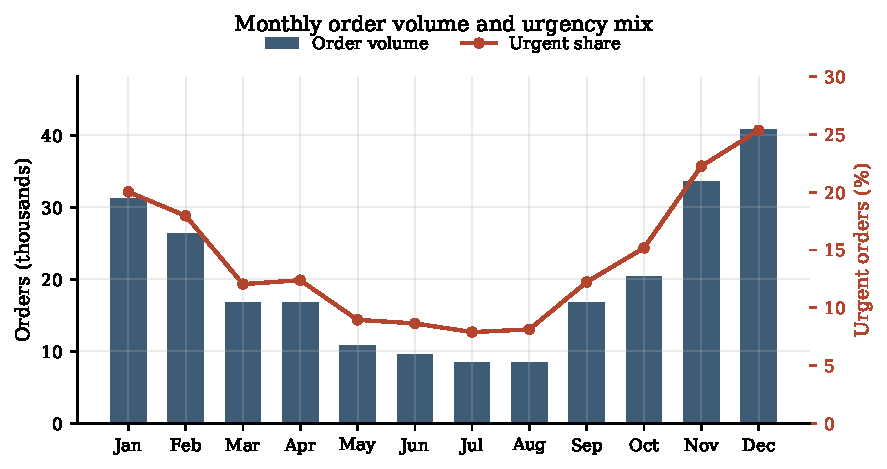
\includegraphics[width=\textwidth]{f1_demand_profile.pdf}
\caption[Monthly order volume and urgency mix]{Monthly order volume and urgency mix in the
dataset used for the retrospective experiments. Volume and urgent share peak together, so the
months with the greatest capacity requirement are also those with the largest proportion of
tightly constrained orders.}
\label{fig:demand}
\end{figure}

\section{Order heterogeneity and the workload model}
\label{sec:order-heterogeneity}

A central modelling choice is that an order is not a unit of work. Each order carries a
\emph{workload unit} value for each of the three stages, computed when the order is created
from its item count and its product attributes:

\begin{equation}
u_{i,s} \;=\; n_i \times \phi_s(\text{family}_i) \times \gamma_s(\text{complexity}_i)
              \times \omega_s(\text{urgency}_i),
\label{eq:workload-units}
\end{equation}

\noindent where \(u_{i,s}\) is the workload of order \(i\) at stage \(s\), \(n_i\) is its item
count, and \(\phi_s\), \(\gamma_s\) and \(\omega_s\) are stage-specific multipliers for product
family, complexity level and urgency respectively.

The multipliers are what make the model interesting, because they differ across stages. A
\emph{fragile} order carries a multiplier of \num{1.1} at picking but \num{1.8} at packing:
fragile goods are not much harder to retrieve, but they are considerably harder to pack safely.
A \emph{bulky} order is relatively harder at picking (\num{1.3}) than the fragile one, but less
demanding at packing (\num{1.6}) than fragile. Urgency multiplies workload only at dispatch
(\num{1.3} for urgent orders, \num{1.0} otherwise), reflecting the additional handling that
expedited shipments require at the point of release. The full multiplier set is reproduced in
\Cref{app:B}.

The consequence is that the three stages do not see proportional workload. Across the dataset
the mean workload per order is \num{3.39} units at picking, \num{2.46} at packing and
\num{1.17} at dispatch --- a ratio of roughly \(1 : 0.72 : 0.34\) --- and, as
\Cref{fig:stage-workload} shows, that ratio itself shifts through the year as the product and
complexity mix changes. A capacity model that treated an order as one unit of work at every
stage would mis-size at least two of the three stages, and would mis-size them differently in
different months.

\begin{figure}[htbp]
\centering
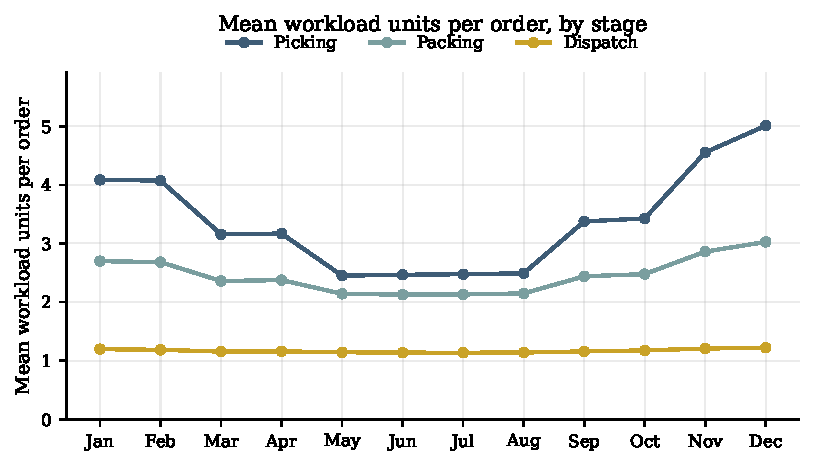
\includegraphics[width=\textwidth]{f2_stage_workload.pdf}
\caption[Mean workload units per order by stage]{Mean workload units per order at each stage,
by month. The three stages are loaded very differently by the same order stream, and the
relationship between them changes seasonally as the product mix shifts.}
\label{fig:stage-workload}
\end{figure}

\subsection{Service times}

Workload units are converted into service time at execution:

\begin{equation}
t_{i,s} \;=\; \max\!\left(t^{\min}_s,\; \left(b_s + c_s\, u_{i,s}\right) \cdot \varepsilon\right),
\qquad
\varepsilon \sim \operatorname{clip}\!\left(\mathcal{N}(1,\,0.12),\; 0.80,\; 1.25\right),
\label{eq:service-time}
\end{equation}

\noindent where \(b_s\) is a fixed set-up component, \(c_s\) the marginal minutes per workload
unit, and \(\varepsilon\) a clipped multiplicative noise term. The parameters are
\(b_s = \SI{0.5}{\minute}\) at all three stages, with
\(c_{\text{pick}} = 0.90\), \(c_{\text{pack}} = 0.70\) and \(c_{\text{disp}} = 0.65\) minutes
per unit, and \(t^{\min}_s = \SI{0.2}{\minute}\).

Two assumptions are embedded here. The fixed component \(b_s\) represents the per-order
overhead that does not scale with size, so that service time is affine rather than proportional
in workload. The clipped normal noise represents execution variability while ruling out the
extreme draws that an unbounded distribution would occasionally produce; the clipping bounds
(\num{0.80} to \num{1.25}) keep variability within a range plausible for repetitive manual
work. The distribution is an assumption of the model, not an empirical fit --- no real handling
time data were available to fit against, and this is noted as a limitation.

\section{The operating-time abstraction}
\label{sec:operating-time}

\subsection{The problem it solves}

A monthly capacity plan must reconcile two quantities that are easy to state separately and
easy to get wrong together: the hours a worker is physically available to process work, and
the hours the organisation pays for. If demand is spread across a calendar month of roughly
\SI{744}{\hour} while labour cost is computed against \SI{160}{\hour} of paid capacity, then
each simulated worker receives several hundred hours of unpaid processing capacity, and every
resulting capacity recommendation is optimistic.

The framework resolves this by defining a single \emph{operating horizon}:

\begin{equation}
H \;=\; h \times 60 \;=\; 160 \times 60 \;=\; \SI{9600}{\minute},
\label{eq:horizon}
\end{equation}

\noindent where \(h\) is the paid productive hours per worker per month. One worker unit
therefore represents exactly \SI{9600}{} productive worker-minutes, and this same \(h\) appears
in the labour cost of \Cref{eq:cost}. Physical capacity and paid capacity are the same quantity
by construction.

\subsection{How calendar demand is mapped onto it}

Calendar arrival timestamps are compressed onto the operating horizon by a linear rescale
within each order's own calendar month:

\begin{equation}
\tau_i \;=\; \frac{t_i - t^{\text{start}}_{m(i)}}
                  {t^{\text{end}}_{m(i)} - t^{\text{start}}_{m(i)}} \times H,
\label{eq:compression}
\end{equation}

\noindent where \(t_i\) is the calendar arrival time of order \(i\), \(m(i)\) its month, and
\(\tau_i\) its position on the operating clock. Because the mapping is a monotone linear
rescale within a month, the relative ordering of arrivals and the burstiness of the arrival
pattern are preserved exactly; what is not preserved is literal wall-clock time.

This matters for interpretation. The statement ``the warehouse operates \SI{160}{\hour} per
month'' would be wrong. The correct statement is that \SI{160}{\hour} is the monthly productive
capacity of one full-time equivalent, and that demand is evaluated against that capacity with
its temporal shape intact. \Cref{fig:compression} illustrates the mapping.

\begin{figure}[htbp]
\centering
\begin{tikzpicture}[x=0.88cm, y=1cm]
  % calendar axis
  \draw[thick, draw=black!60] (0,2.2) -- (12,2.2);
  \coordinate (calleft) at (0,2.2);
  \node[note, left=2pt of calleft, anchor=east] {calendar\\month};
  \foreach \x in {0,1,...,12} \draw[draw=black!45] (\x,2.1) -- (\x,2.3);
  \node[font=\scriptsize, below=1pt] at (0,2.1) {day 1};
  \node[font=\scriptsize, below=1pt] at (12,2.1) {day 31};

  % a few arrivals, clustered to show burstiness is preserved
  \foreach \x in {0.6, 1.1, 1.35, 4.2, 6.5, 6.8, 7.0, 9.4, 10.6, 10.9, 11.2}
    \fill[thesisblue] (\x,2.2) circle (1.5pt);

  % operating axis
  \draw[thick, draw=thesisblue] (0,0) -- (12,0);
  \coordinate (opleft) at (0,0);
  \node[note, left=2pt of opleft, anchor=east, text=thesisblue]
       {operating\\horizon $H$};
  \node[font=\scriptsize, below=1pt] at (0,-0.05) {$0$};
  \node[font=\scriptsize, below=1pt] at (12,-0.05) {\SI{9600}{\minute}};
  \foreach \x in {0.6, 1.1, 1.35, 4.2, 6.5, 6.8, 7.0, 9.4, 10.6, 10.9, 11.2}
    \fill[thesisblue] (\x,0) circle (1.5pt);

  % mapping arrows
  \foreach \x in {0.6, 1.35, 4.2, 6.8, 9.4, 11.2}
    \draw[-{Stealth[length=1.6mm]}, draw=black!40] (\x,2.1) -- (\x,0.12);

  \coordinate (midright) at (12,1.1);
  \coordinate (below) at (6,-0.1);
  \node[note, right=0.1cm of midright, anchor=west, text width=1.9cm]
       {linear\\rescale};
  \node[note, below=0.55cm of below, text width=12cm]
       {relative ordering and burstiness preserved exactly $\cdot$ wall-clock time not preserved};
\end{tikzpicture}
\caption[Operating-time compression]{Compression of calendar arrivals onto the operating
horizon. Each order's position within its own calendar month is rescaled linearly onto
\([0, H)\), so the shape of demand --- including bursts --- is retained while the clock is
decoupled from calendar time.}
\label{fig:compression}
\end{figure}

\subsection{Consequences for the service-level clock}
\label{sec:sla-clock}

Because the simulation runs on the operating clock, service-level thresholds are measured in
\emph{productive elapsed minutes}. The configured thresholds are \SI{240}{\minute} for urgent
orders and \SI{1440}{\minute} for normal orders. These should be read as service targets on the
operating-time scale, not as literal promises of four hours and twenty-four hours of wall-clock
time to the customer. Mapping them onto real delivery promises would require the calendar
structure of a specific operation --- its shift pattern, its cut-off times and its carrier
schedule --- which is outside the scope of this study.

\subsection{The finite horizon and backlog}
\label{sec:finite-horizon}

The simulation runs for exactly \(H\) minutes and then stops. It does not continue until all
orders are complete. Orders still queued or in service when the horizon ends are treated as
\emph{backlog}: their system time is undefined, they are counted as service-level failures, and
they are additionally reported separately as an unfinished-order count and a backlog share.

This is a deliberate design choice with a clear rationale. If the simulation ran until the last
order finished, an under-staffed configuration would eventually complete all its work and could
report a respectable service level, simply by processing December's orders into what would in
reality be January. The finite horizon prevents insufficient capacity from being concealed by
unlimited post-period processing, and makes the accumulated backlog visible as a distinct
quantity that a planner can reason about.

\section{The discrete-event simulation engine}
\label{sec:des-engine}

\subsection{Why discrete-event simulation}

The choice of discrete-event simulation follows from the structure of the problem rather than
from methodological preference. The quantities that determine whether a workforce configuration
succeeds --- when queues form, how long orders wait, how congestion at one stage propagates to
the next, how much work remains at the end of the month --- are emergent consequences of
individual arrival and service events interacting with finite capacity. They are not available
in closed form for a system with this combination of features: non-stationary bursty arrivals,
heterogeneous and stage-differentiated service requirements, multiple servers per stage, a
sequencing decision at every stage, and two customer classes with different deadlines.

An analytical treatment would require assumptions --- stationarity, exponential service,
class-independent workload --- that remove exactly the features under study. Discrete-event
simulation makes no such assumptions, at the cost of producing estimates rather than closed-form
results \citep{law2015}. The framework therefore uses both: an analytical estimate as a cheap
screening anchor (\Cref{sec:capacity-estimate}), and simulation as the arbiter.

\subsection{Model structure}

The model is implemented in Python using the SimPy process-based simulation library. Orders
arrive according to their compressed operating-time timestamps, join the picking queue, are
served by one of the picking workers, then pass in turn to packing and dispatch. Each stage has
its own queue and its own worker pool; workers are not shared across stages, and queues are
unbounded, so there is no blocking. \Cref{fig:flow} shows the structure.

The state recorded for each order is the set of timestamps at which it entered and left service
at each stage. From these, all reported metrics are derived: system time, service-level
attainment, per-stage waiting time distributions, per-stage utilisation and busy time. Queue
lengths are tracked separately by an event-driven accumulator that records the exact moments at
which a queue gains or loses an item, giving an exact time-weighted average queue length rather
than a sampled approximation.

Utilisation at a stage is computed as busy worker-minutes over available worker-minutes:

\begin{equation}
\rho_s \;=\; \frac{\sum_{i} t_{i,s}}{w_s \cdot H},
\label{eq:utilisation}
\end{equation}

\noindent where \(w_s\) is the number of workers at stage \(s\). Because a worker cannot be
busy for longer than the horizon, a value above \num{1} would indicate an error rather than a
meaningful result, and the implementation raises a warning if one occurs.

\section{The sequencing policies as implemented}
\label{sec:policies}

Three policies are compared. Two are transparent heuristics and one is learned. Because the
precise semantics of these policies determine how the results in \Cref{ch:results} must be
read, each is described exactly as implemented rather than by its conventional definition.

\subsection{FIFO}

Under FIFO each stage holds a single first-in-first-out queue, and workers take the order that
has been waiting longest at that stage. It is important to note that this is
\emph{stage-local}. At picking, queue order is customer arrival order. At packing and dispatch,
it is the order in which upstream work was completed, which need not coincide with arrival
order because service times differ between orders. FIFO in this model therefore means
``first to become available at this stage is first served here'', not ``first ordered by the
customer is first served everywhere''.

FIFO is included as the neutral baseline: it makes no use of the urgency information attached
to an order, and therefore shows what happens when differentiated service commitments are not
reflected in the operating discipline.

\subsection{Urgent-First}
\label{sec:urgent-first}

Under Urgent-First each stage holds a single priority queue, with urgent orders assigned
priority \num{0} and normal orders priority \num{1}. Workers always take an order of the
highest available priority, so every waiting urgent order is served before any normal order.
The policy is non-pre-emptive: an order already in service is never interrupted.

The within-class behaviour requires a precise statement, because it differs from what the name
would conventionally suggest. The priority queue is implemented as a binary heap over
priority-tagged items whose comparison operator considers \emph{only} the priority field. Two
orders of the same class are therefore never ordered relative to one another, and the sequence
in which equal-priority orders leave the queue is determined by the internal structure of the
heap. It is deterministic given the insertion sequence, but it is neither first-in-first-out
nor sorted by order identifier.

This was confirmed by direct observation rather than inferred from the source: inserting ten
equal-priority items in the order \(1,2,\dots,10\) returns them in the order
\(1, 3, 7, 10, 9, 6, 8, 5, 2, 4\). The same check confirms that the class-level priority
\emph{is} strictly respected --- all urgent orders precede all normal orders. The verification
script is described in \Cref{app:E}.

The correct characterisation of this policy is therefore: \emph{strict two-class priority with
unspecified within-class ordering}. This is not a defect to be corrected but a property of the
baseline that must be carried into the interpretation of the results, and
\Cref{sec:disc-policy} returns to it when accounting for the very large p95 waiting times that
Urgent-First produces for the normal class.

\subsection{RL-3}
\label{sec:rl3}

The third policy replaces the fixed rule with a learned one. Under RL-3 each stage holds
\emph{two} first-in-first-out queues, one per class, and a reinforcement learning agent decides
which of the two to serve whenever a worker becomes free.

\paragraph{Agent and scope.} A single deep Q-network \citep{mnih2015} is shared across all
three stages. It is not three separate agents: the same network parameters make the decision at
picking, packing and dispatch, with the identity of the stage supplied as an input feature.
This design isolates the effect of acting at every stage with one consistent policy.

\paragraph{Decision points.} The agent is consulted only when \emph{both} queues at a stage are
non-empty, that is, only when there is a genuine choice to make. If exactly one class is
waiting, the action is forced and the resulting transition is not stored for training, so the
agent is not trained on decisions it did not make.

\paragraph{Actions.} There are two actions: action \num{0} serves the urgent queue and action
\num{1} serves the normal queue. Within the chosen class, service is first-in-first-out ---
which, as noted above, differs from the Urgent-First baseline's within-class behaviour. The two
engines implement different queue mechanics by design, and the comparison is between the
decision rules as implemented.

\Cref{fig:rl-structure} summarises the decision structure.

\begin{figure}[htbp]
\centering
\begin{tikzpicture}[node distance=0.55cm]
  \node[block, minimum width=10.4cm, minimum height=1.0cm] (state)
       {\textbf{state} --- 16 features, all clipped to $[0,1]$\\[1pt]
        \scriptsize six queue lengths $\cdot$ three WIP counts $\cdot$ elapsed time $\cdot$
        head slack (urgent, normal) $\cdot$ stage id $\cdot$ three capacities};

  \node[stage, below=of state, minimum width=3.6cm, minimum height=1.0cm] (dqn)
       {shared DQN};

  \node[block, below=of dqn, minimum width=10.4cm, minimum height=0.95cm] (act)
       {\textbf{action}\quad 0: serve the urgent queue \quad$|$\quad 1: serve the normal queue};

  \node[endnode, below=1.0cm of act, minimum width=10.4cm] (rew)
       {reward assigned at dispatch completion, applied to every decision taken for that order};

  \draw[flow] (state) -- (dqn);
  \draw[flow] (dqn) -- (act);
  \draw[flow, dashed] (act) -- node[note, right=2pt] {deferred} (rew);

  \node[note, above=0.28cm of state, text width=11.5cm]
       {observed at whichever stage is deciding --- consulted only when both queues there
        are non-empty};
  \node[note, right=0.3cm of dqn, text width=4.4cm, anchor=west]
       {the same parameters act at all\\three stages; the stage enters\\as a feature, not as a
        separate agent};
\end{tikzpicture}
\caption[RL-3 decision structure]{The RL-3 decision structure. A single network observes the
present state at whichever stage is deciding and chooses which class to serve; the reward is
deferred until the order leaves the system.}
\label{fig:rl-structure}
\end{figure}

\paragraph{State.} The state is a 16-dimensional vector, all components clipped to
\([0,1]\). It comprises the six queue lengths (urgent and normal at each of the three stages,
normalised by class-specific reference values), the three work-in-progress counts, the fraction
of the horizon elapsed, the normalised slack of the head order in each of the two queues at the
current stage, the stage identifier, and the three normalised worker counts. The complete
specification, including the exact ordering and normalisation of each feature, is given in
\Cref{app:C}.

Two properties of this state deserve emphasis. First, the worker-count features allow the agent
to condition its behaviour on how much capacity is available, so that it need not treat a
tightly constrained configuration identically to a generous one. Second, and more importantly,
\emph{nothing in the state encodes future arrivals}. The agent observes the current queue
state, the current work in progress, the elapsed fraction of the horizon and the urgency of the
orders at the head of each queue. It has no forecast, no lookahead and no privileged
information. Any interpretation of its behaviour as anticipating future demand would be
unsupported.

\paragraph{Reward.} The reward is deferred until an order completes dispatch, at which point
every decision recorded for that order receives the same value:

\begin{equation}
r_i \;=\;
\begin{cases}
w_{c(i)}, & \text{if the order met its service target,}\\[4pt]
-\,p_{c(i)} \cdot \min\!\left(1,\; \dfrac{L_i}{\sigma_{c(i)} \cdot \kappa}\right), & \text{otherwise,}
\end{cases}
\label{eq:reward}
\end{equation}

\noindent where \(c(i)\) is the order's class, \(L_i\) its lateness, \(\sigma_{c(i)}\) its
system-time SLA threshold and \(\kappa\) a cap multiplier. Orders left as backlog at the end of the
horizon receive the full penalty \(-p_{c(i)}\), so that abandoning work is treated as the
service failure it is rather than as a neutral outcome. Coefficient values are given in
\Cref{app:C}.

The structure encodes the intended trade-off: meeting an urgent order's target is worth more
than meeting a normal order's, but the penalty for lateness is the same for both classes, so
the agent has an incentive to protect urgent service without licence to abandon normal service
entirely. Attributing the same terminal reward to every decision along an order's path is an
approximation --- it assumes each decision contributed to the eventual outcome --- and is
recorded as such among the limitations.

\paragraph{Training.} The agent was trained for 200 episodes, each sampling one
(month, workforce configuration) pair uniformly from a fixed training pool, with a learning rate
of \num{1e-3}, discount factor \num{0.99}, batch size \num{256}, a replay buffer of \num{200000}
transitions, a target network updated every \num{2000} steps and \(\varepsilon\)-greedy
exploration annealed from \num{1.0} to \num{0.05}. Training deliberately omits the common random
number mechanism described in \Cref{sec:crn}, so that each training episode encounters
independent service-time realisations. The pool covers three representative months --- June,
October and December, chosen to span low, medium and peak demand --- and, for each, seven
workforce configurations drawn from that month's own candidate neighbourhood, giving 21 training
pairs; two further configurations per month were held out from training entirely.
\Cref{sec:app-training-pool} lists the pool exactly and states what follows from it for
generalisation. Full hyperparameters are in \Cref{app:C}.

\paragraph{Evaluation is greedy.} A distinction that matters for reading every RL-3 figure in
this thesis: exploration is a training device only. Every evaluation run --- the retrospective
grid, the forecast replications and the diagnostics --- invokes the network in greedy mode,
taking the action of maximum estimated value with no random component, and records no training
transitions. The \(\varepsilon\)-greedy schedule above applies during training and nowhere else.
No reported RL-3 metric contains randomly chosen exploratory actions.

\section{Analytical capacity estimate}
\label{sec:capacity-estimate}

Before any simulation is run, an analytical estimate provides a starting point for the search.
For each stage, the expected deterministic workload is divided by the effective capacity of one
worker and rounded up:

\begin{equation}
\hat{w}_s \;=\; \max\!\left(1,\; \left\lceil
\frac{\sum_i \left(b_s + c_s\, u_{i,s}\right)}{H \cdot \upsilon}
\right\rceil\right),
\label{eq:capacity-estimate}
\end{equation}

\noindent where \(\upsilon = 0.85\) is a target utilisation and the noise term of
\Cref{eq:service-time} is fixed at its mean of \num{1}. The target utilisation is a deliberate
safety margin: sizing to \SI{100}{\percent} of capacity would guarantee unbounded queueing in
any system with variability \citep{hopp2011}.

This estimate is an \emph{anchor}, not a recommendation. It knows nothing about queueing
dynamics, sequencing or class-specific service requirements, and \Cref{sec:res-capacity} shows
that it systematically differs from what simulation actually recommends. Its role is to place
the search in the right region of the space so that a bounded set of candidates suffices.

\section{Dynamic candidate generation}
\label{sec:candidates}

Around the analytical centre \((\hat{w}_{\text{pick}}, \hat{w}_{\text{pack}},
\hat{w}_{\text{disp}})\), the framework generates a bounded set of 16 distinct workforce
candidates in a fixed, deterministic order: the centre itself; the client's current workforce
if one was supplied; single-stage perturbations of \(\pm 1\); leaner and safer variants scaling
the whole workforce by \(\mp\SI{15}{\percent}\); balanced two-stage combinations; and finally
single-stage perturbations of \(\pm 2\) if the budget of 16 allows. Every stage is clamped to at
least one worker.

This is a \emph{structured neighbourhood search}, and it is important not to overstate it. It
is not a full grid --- a cubic grid over a plausible range would be prohibitively expensive at
these order volumes --- and it is not global optimisation. There is no guarantee that the best
configuration in the whole space lies within the 16 evaluated. The design trades that guarantee
for tractability, on the reasoning that the analytical anchor places the neighbourhood in a
sensible region and that a planner is choosing among operationally plausible configurations
rather than searching an unbounded space.

Configurations are labelled \rgm{sPKD} for single-digit worker counts and \rgm{sP\_K\_D}
otherwise, as described in the front matter.

\section{Service-level feasibility}
\label{sec:feasibility}

A configuration is \emph{feasible} if and only if it satisfies both class-specific service
floors:

\begin{equation}
\text{feasible} \iff
\left(\text{SLA}_{\text{urgent}} \geq 0.95\right) \;\wedge\;
\left(\text{SLA}_{\text{normal}} \geq 0.80\right).
\label{eq:feasibility}
\end{equation}

The conjunction is the essential point. An aggregate service criterion would be satisfied by
configurations that are operationally unacceptable, because the urgent class is a minority of
volume and its failures are therefore diluted. The results provide a direct illustration: in
October at configuration \rgm{s753}, FIFO achieves \SI{81.0}{\percent} aggregate service
attainment --- a figure that sounds tolerable --- while delivering only \SI{24.5}{\percent}
attainment to the urgent class. Any criterion that reported the aggregate alone would have
accepted that configuration.

Where a configuration is infeasible, the magnitude of failure is summarised by a transparent
violation score, the sum of the two shortfalls, each floored at zero.

\subsection{The recommendation rule as implemented}
\label{sec:selection-rule}

Feasibility is what turns the simulated grid into a recommendation, and the rule that does so is
worth stating exactly, because it is lexicographic rather than a plain cost minimisation.

For a given month the framework holds one simulated row per (configuration, policy) pair. It
then applies, in order:

\begin{enumerate}
  \item \textbf{Eligibility.} In forecast mode, only rows carrying a full three-replication
        aggregate are eligible; single-replication screening rows are retained for diagnostic
        display but can never become the recommendation. In retrospective mode every row is
        eligible.
  \item \textbf{Feasibility first.} If any eligible row satisfies both service floors, the
        recommendation is the cheapest such row by total cost. Infeasible rows are excluded
        entirely at this step, however cheap they are.
  \item \textbf{Fallback.} If no eligible row satisfies both floors, the recommendation is the
        row with the smallest service violation, ties broken by lowest total cost. The output is
        then reported as infeasible.
\end{enumerate}

The fallback branch is stated rather than hidden because it changes how such a recommendation
should be read: it is the least-bad configuration among those examined, not a plan that meets
the commitments. In the retrospective run reported in \Cref{ch:results} the fallback was never
reached --- a feasible row existed in all twelve months --- but the framework's behaviour when
it does not is part of the specification.

One reporting distinction follows from this and is easy to conflate. Alongside the
recommendation, the export layer publishes several \emph{descriptive} per-month statistics for
comparison: the cheapest configuration overall, the smallest configuration meeting both floors,
the smallest meeting the urgent floor alone, and the best result for each individual policy. The
first of these is computed without a feasibility filter and is a summary statistic, not the
selection rule. \Cref{sec:app-rules} tabulates them, and \Cref{tab:recommendations} notes which
column it reports.

\section{Economic model}
\label{sec:economics}

Total monthly cost combines labour and the penalty cost of late orders:

\begin{equation}
C \;=\; \underbrace{\left(w_{\text{pick}} + w_{\text{pack}} + w_{\text{disp}}\right) \cdot k \cdot h}_{\text{labour}}
\;+\; \underbrace{n^{\text{late}}_{\text{urgent}} \cdot \pi_{\text{urgent}}
\;+\; n^{\text{late}}_{\text{normal}} \cdot \pi_{\text{normal}}}_{\text{service failure}},
\label{eq:cost}
\end{equation}

\noindent where \(k\) is the hourly labour cost, \(h\) the paid hours per worker-month, and
\(\pi_c\) the penalty per late order of class \(c\). The same \(h\) appears here and in
\Cref{eq:horizon}, which is the point of the operating-time design.

These values are \emph{scenario assumptions}, supplied at run time, not empirically estimated
parameters. This has an important consequence for how results may be compared. The two
experimental runs reported in this thesis were executed with different economic assumptions:
the retrospective run used \(\pi_{\text{urgent}} = 20\), \(\pi_{\text{normal}} = 5\) and
\(k = 15\); the forecast run used \(\pi_{\text{urgent}} = 15\),
\(\pi_{\text{normal}} = 10\) and \(k = 18\). Each run is therefore reported \emph{as run}, and
\textbf{no absolute monetary comparison is drawn between the two modes} anywhere in this
thesis. Within a run, all comparisons share a common parameter set and are valid.

\section{Stage Pressure: the bottleneck diagnostic}
\label{sec:stage-pressure}

Identifying which stage constrains the operation is a prerequisite for explaining a
recommendation. The framework combines four normalised signals into a single comparable score
per stage:

\begin{equation}
P_s \;=\; 0.40\,\rho_s \;+\; 0.25\,\widetilde{q}^{\,95}_s \;+\; 0.20\,\lambda_s
      \;+\; 0.15\,\widetilde{\ell}_s,
\label{eq:pressure}
\end{equation}

\noindent where \(\rho_s\) is utilisation, \(\widetilde{q}^{\,95}_s\) the p95 waiting time,
\(\lambda_s\) the share of late orders' accumulated waiting time attributable to stage \(s\),
and \(\widetilde{\ell}_s\) the time-weighted average queue length.

The normalisation is not uniform across terms, and describing it accurately matters.
Utilisation enters as an absolute ratio clipped to \([0,1]\), so it is comparable across
scenarios. The p95 waiting time and average queue length are normalised \emph{by the maximum
across the three stages}, so they are relative signals: the most-pressured stage always scores
\num{1.0} on those two components regardless of the absolute values. The late-order waiting
share is already a proportion summing to one across stages. A pressure score is therefore
meaningful for \emph{ranking stages within a scenario}, and should not be compared as an
absolute quantity across scenarios.

\subsection{Why these four signals, and why these weights}

The rationale is operational rather than statistical. Utilisation carries the largest weight
because it is the most direct measure of capacity pressure and the quantity most directly
addressed by adding a worker. The p95 waiting time captures the tail of the waiting
distribution, which is what determines service failures --- a stage can have a modest average
wait and still generate late orders through its tail. The late-order waiting share attributes
observed failures to the stage where the waiting actually accumulated, connecting the diagnostic
to the outcome the planner cares about. Average queue length adds evidence of sustained work
accumulation as opposed to transient spikes. The remaining three weights are ordered to reflect
that decreasing directness of evidence.

It must be stated plainly what this score is not. The weights were \emph{not} obtained by
optimisation, statistical calibration or expert elicitation; they are a transparent heuristic
chosen for interpretability. The score does not establish causality: it identifies where
pressure is concentrated, not what causes any individual order to be late. The appropriate
phrasing --- used throughout \Cref{ch:results} --- is that a stage is ``identified as the
primary pressure location under the diagnostic'', not that it causes the failures observed.

\section{Adaptive capacity search}
\label{sec:adaptive}

The bottleneck diagnostic feeds a further step, but not unconditionally. The search is triggered
only when there is a reason to believe additional capacity might help: either the recommended
configuration is infeasible, or its primary pressure stage runs at \SI{85}{\percent} utilisation
or above \emph{and} late orders are already occurring. Where a recommendation is comfortably
feasible at moderate utilisation, no candidate is constructed and no additional simulation is
spent.

When it is triggered, the framework ranks the stages by pressure and constructs a neighbouring
candidate with one additional worker at the most pressured stage. If the second-ranked stage scores within a configured margin of the
first --- \num{0.05} on the pressure scale --- a candidate is constructed for that stage as
well, so that a near-tie in the diagnostic is resolved by simulation rather than by the score
alone. At most two candidates are tested per iteration, and no stage may be raised beyond its
own analytical estimate plus four workers.

Each candidate is re-simulated under all three policies and compared against the incumbent by an
acceptance rule with three branches, evaluated in order:

\begin{enumerate}
  \item if the incumbent is infeasible and the candidate is feasible, accept --- reaching the
        service floors takes precedence over cost;
  \item if both are feasible and the candidate's total cost is lower, accept;
  \item if both are infeasible but the candidate's service violation is smaller, accept it as
        an improvement towards feasibility.
\end{enumerate}

\noindent Otherwise the candidate is rejected and the incumbent stands. Where the rejection
arises because the candidate is no cheaper, the recorded reason is that the added labour cost
was not offset by the reduction in late-order penalties --- which is the outcome observed
throughout \Cref{sec:res-bottleneck}.

The ordering of these branches matters for interpretation, and it is worth being precise about
it. The procedure is \emph{not} a pure cost minimisation. An additional worker that converts an
infeasible configuration into a feasible one is accepted whatever it costs, because an
infeasible plan is not a plan at all. Cost becomes the deciding criterion only once the service
commitments are already satisfied. After each acceptance the bottleneck ranking is recomputed
from the new incumbent, so successive iterations may address different stages. The procedure
runs for at most four iterations and stops when no tested neighbour improves the objective or
when the per-stage ceilings are reached.

The forecast workflow applies the same acceptance rule with an additional screening step: a
candidate is first evaluated on a single replication, and only if it looks promising is it
validated across all replications before the decision is finalised. This prevents a candidate
assessed on one replication from displacing an incumbent that was validated on three.

The managerial content of this step is worth making explicit, because it is easily
misinterpreted. Identifying a bottleneck is often treated as equivalent to recommending
additional capacity there. It is not. An additional full-time equivalent has a definite monthly
cost, and whether it pays for itself depends on how many service failures it actually prevents
--- a quantity that cannot be read off the bottleneck ranking and must be obtained by
simulating the alternative. \Cref{sec:res-bottleneck} shows that in this study the test was
applied in nine months and the additional worker was rejected in every one of them.

As with the candidate search, this is not optimisation. It is a bounded local improvement step
with an explicit, documented acceptance rule. \Cref{fig:adaptive} shows the loop.

\begin{figure}[htbp]
\centering
\begin{tikzpicture}[node distance=0.5cm]
  \node[block, minimum width=6.8cm] (rec) {recommended configuration from the candidate search};
  \node[block, below=of rec, minimum width=6.8cm] (trig)
       {\textbf{trigger?} infeasible, \emph{or} bottleneck utilisation $\geq \SI{85}{\percent}$
        with late orders};
  \node[block, below=of trig, minimum width=6.8cm] (rank)
       {rank stages by pressure $\rightarrow$ add 1 FTE at the top stage\\[-1pt]
        \scriptsize (and at the second stage if within \num{0.05})};
  \node[block, below=of rank, minimum width=6.8cm, fill=thesisblue!7, draw=thesisblue] (sim)
       {re-simulate the candidate under all three policies};
  \node[block, below=of sim, minimum width=6.8cm] (dec)
       {\textbf{accept?} feasibility gained $\rightarrow$ yes;\ \ cheaper and feasible
        $\rightarrow$ yes;\\[-1pt] smaller violation $\rightarrow$ yes;\ \ otherwise no};
  \node[endnode, below=of dec, minimum width=6.8cm] (fin)
       {final recommendation};

  \foreach \a/\b in {rec/trig, trig/rank, rank/sim, sim/dec}
    \draw[flow] (\a) -- (\b);
  \draw[flow] (dec) -- node[note, right=1pt, pos=0.45] {reject} (fin);
  \draw[flow] (trig.east) -- ++(0.7,0) |- node[note, right=1pt, pos=0.25] {no} (fin.east);
  \draw[flow] (dec.west) -- ++(-0.8,0) |- node[note, left=1pt, pos=0.25] {accept:\\re-rank} (rank.west);
\end{tikzpicture}
\caption[Adaptive capacity search]{The adaptive capacity loop. Additional capacity at the
identified bottleneck is proposed, simulated and then accepted or rejected on explicit
criteria; feasibility takes precedence over cost.}
\label{fig:adaptive}
\end{figure}

\section{Experimental design}
\label{sec:experimental-design}

\subsection{Common random numbers}
\label{sec:crn}

Comparing sequencing policies fairly requires that they face the same work. This is not
automatic: because the policies dequeue orders in different sequences, an engine that sampled
service times as orders entered service would advance its random number stream differently
under each policy, and the same nominal seed would produce different service times.

The framework avoids this by pre-computing a service-time map. For a given scenario seed, the
service time of every (order, stage) pair is drawn once, iterating orders in identifier order
and stages in fixed order, before any policy runs. All three policies then look up the same
map. Order \num{4711} therefore requires exactly the same picking minutes under FIFO, under
Urgent-First and under RL-3; what differs between policies is solely \emph{when} that work is
done, which is precisely the effect under study.

This is the classical variance reduction technique of common random numbers
\citep{law2015}. Its benefit here is that differences observed between policies are attributable
to the sequencing decision rather than to sampling noise, which allows meaningful comparison
without large numbers of replications. \Cref{fig:crn} shows the arrangement.

\begin{figure}[htbp]
\centering
\begin{tikzpicture}[node distance=0.55cm and 0.9cm]
  \node[block, minimum width=8.6cm, fill=thesisblue!8, draw=thesisblue] (map)
       {\textbf{Service-time map}\\[-1pt]
        \footnotesize drawn once per scenario seed, for every (order, stage) pair};

  \node[stage, below=1.25cm of map, minimum width=2.5cm] (uf) {Urgent-First};
  \node[stage, left=of uf,  minimum width=2.5cm] (fifo) {FIFO};
  \node[stage, right=of uf, minimum width=2.5cm] (rl) {RL-3};

  \foreach \p in {fifo,uf,rl} \draw[flow] (map) -- (\p);

  \node[note, below=0.06cm of fifo, text width=2.5cm] {different\\dequeue order};
  \node[note, below=0.06cm of uf,   text width=2.5cm] {different\\dequeue order};
  \node[note, below=0.06cm of rl,   text width=2.5cm] {different\\dequeue order};

  \node[note, above=0.28cm of map, text width=11.5cm, text=black!70]
       {orders iterated in identifier order, stages in fixed order ---
        the map depends only on (orders, seed), never on the policy};
  \node[endnode, below=2.1cm of uf, minimum width=10.2cm] (concl)
       {identical service time per order and stage across all three policies};
  \coordinate (bus) at ([yshift=0.5cm]concl.north);
  \draw[draw=black!70, thick] (fifo.south |- bus) -- (rl.south |- bus);
  \foreach \p in {fifo,rl} \draw[draw=black!70, thick] (\p.south) -- (\p.south |- bus);
  \draw[draw=black!70, thick] (uf.south) -- (uf.south |- bus);
  \draw[flow] (uf.south |- bus) -- (concl.north);
\end{tikzpicture}
\caption[Common random numbers design]{The common random number arrangement. Service times are
drawn once per scenario seed, before any policy runs, and looked up by all three. What differs
between policies is only \emph{when} each unit of work is done.}
\label{fig:crn}
\end{figure}

\subsection{The two workflows}

The framework was exercised in both of its modes, and their designs differ.

The \textbf{retrospective} workflow processed all twelve months of the order-level dataset. For
each month it computed the analytical estimate, generated 16 candidates, and evaluated every
candidate under all three policies --- \(12 \times 16 \times 3 = 576\) simulation runs --- with
one scenario seed per month. Its question is counterfactual: \emph{given the demand that
occurred, which workforce configuration and sequencing policy would the framework have
recommended?} It does not claim that the recommended workforce was the one actually used.

The \textbf{forecast} workflow was exercised on December, the peak month. Starting from an
aggregate expected volume and an uncertainty level, it generated three stochastic replications
of the month's orders and applied a two-stage evaluation. Stage~A screened all 16 candidates
under all three policies on the first replication (\(16 \times 3 \times 1 = 48\) runs); Stage~A
then ranked the configurations and retained four finalists, which Stage~B extended to the two
remaining replications (\(4 \times 3 \times 2 = 24\) further runs). The total is 72 simulation
runs rather than the 144 a full three-replication evaluation would have required, a reduction
of \SI{50}{\percent}. Only the finalists' three-replication aggregates are eligible to become
the recommendation. This produces evidence across scenarios --- a mean cost, the spread across
the three replications and the share of replications in which the service floors were met ---
rather than a single point estimate. Three replications describe that spread; they do not
estimate a distribution, and \Cref{sec:res-future} states the consequences for how the reported
p90 cost and replication success rate should be read.

The asymmetry between the two workflows is a property of the experiments as executed and is
carried into the interpretation: the retrospective results cover a full year at one realisation
per month, while the forecast results cover one month at three replications. They answer
different questions and are not pooled.

\subsection{Forecast scenario generation and uncertainty}
\label{sec:future-uncertainty}

Because RQ4 concerns the \emph{difference} between the two uncertainty structures, the forecast
side deserves to be described mechanically rather than in summary. What follows is the
procedure as implemented.

\paragraph{Inputs.} The forecast entry point takes a planning month, an expected annual order
volume (or a direct monthly override), and a named uncertainty level. The expected monthly
volume is the annual figure multiplied by that month's configured share of the year --- for
December, \num{0.170}. The reported run used the \code{standard} level.

\paragraph{What the uncertainty level is.} An uncertainty level is a pair of configured
coefficients of variation, one for volume and one for the within-month arrival pattern:

\begin{center}
\begin{tabular}{lrr}
\toprule
\textbf{Level} & \textbf{Demand CV} & \textbf{Arrival CV} \\
\midrule
\code{low}      & \num{0.05} & \num{0.15} \\
\code{standard} & \num{0.10} & \num{0.30} \\
\code{high}     & \num{0.20} & \num{0.50} \\
\bottomrule
\end{tabular}
\end{center}

These are \emph{scenario assumptions supplied to the model}, not forecast errors estimated from
any observed forecasting record. Nothing in this study calibrates them against how wrong a real
demand forecast turns out to be. They describe how much variation the planner wishes to test
against, and the reliability figures the workflow reports are conditional on that choice. This
is the sense in which the forecast workflow is a robustness instrument rather than a predictive
one, and it is why \Cref{sec:future-work} identifies propagating genuine forecast error as an
extension rather than a refinement.

\paragraph{How a replication is generated.} Replication \(r\) of month \(m\) is seeded
deterministically as \(42 + 10m + 1000r\), so the three December replications are reproducible
and mutually independent draws. Within a replication:

\begin{enumerate}
  \item \textbf{Volume.} The month's order count is drawn from a lognormal distribution whose
        logarithmic parameters are set so that its mean is the expected monthly volume and its
        coefficient of variation is the level's demand CV. Volume therefore varies from
        replication to replication around the forecast rather than being fixed at it.
  \item \textbf{Arrival pattern.} Daily arrival weights start from the configured calendar
        profile, including the campaign-burst pattern that applies to December, and are then
        multiplied by positive lognormal noise of unit mean whose dispersion is the level's
        arrival CV. This adds day-to-day dispersion on top of the seasonal shape without
        altering the intraday profile.
  \item \textbf{Composition.} Each order's urgency class, product family, complexity level and
        item count are drawn from the same month-specific distributions used by the annual
        generator (\Cref{sec:order-heterogeneity}), and its stage workload units are computed by the
        same rules. The forecast and retrospective streams therefore share a structure while
        being distinct realisations.
\end{enumerate}

\paragraph{What is held common and what varies.} Within one replication, all sixteen
configurations and all three policies are evaluated against exactly the same order stream, and
service times are drawn once per (order, stage) from the common random number map of
\Cref{sec:crn}. Comparisons \emph{within} a replication are therefore matched. Across
replications, everything demand-side changes together: the sampled volume, the arrival pattern
and the individual orders. The variation the reported figures express is thus scenario
variation, not measurement noise on a fixed scenario.

\paragraph{How the four finalists are chosen.} After Stage~A, configurations are ranked using
only replication-1 evidence, by a rule that mirrors the recommendation hierarchy of
\Cref{sec:selection-rule}. A configuration at which \emph{any} policy meets both service floors
ranks ahead of every configuration at which none does, and among those it is ranked by the total
cost of its cheapest feasible policy. Configurations with no feasible policy are ranked after
them, by service violation first and cost second. The four highest-ranked configurations are
carried into Stage~B. The rule operates on configurations, not on (configuration, policy) pairs,
so a finalist carries all three of its policies forward.

\section{Verification and validation}
\label{sec:verification}

Following \citet{sargent2008}, verification and validation are treated as distinct activities.

\textbf{Verification} asks whether the model behaves as designed. Several checks support this.
Utilisation is asserted not to exceed one, which would indicate a worker busy longer than the
horizon. Backlog is confirmed to be a genuine unresolved queue rather than a deadlock: the
horizon timeout guarantees termination regardless of how much work remains. The common random
number mechanism was checked by confirming that service-time lookups depend only on order
identifier, stage and seed. The within-class ordering of the Urgent-First priority queue was
established by direct observation rather than assumption, as described in
\Cref{sec:urgent-first}. Repository-level consistency checks and an audit of the learning agent
are documented in \Cref{app:E}.

An important consequence of the verification stance adopted here is that verification does
\emph{not} license redesign. Where two components were found to implement different queue
mechanics --- the Urgent-First baseline using one priority heap per stage, RL-3 using two
first-in-first-out queues per stage --- the difference is documented as a design fact and
carried into interpretation, not eliminated to make the two engines symmetric.

\Cref{tab:verification} sets out the checks performed and what each establishes.

\begin{table}[htbp]
\centering
\caption[Verification checks]{Verification checks performed, and what each establishes.}
\label{tab:verification}
\small
\begin{tabularx}{\textwidth}{lXX}
\toprule
\textbf{Check} & \textbf{Method} & \textbf{Establishes} \\
\midrule
Utilisation bound & assertion that busy minutes do not exceed worker-minutes available &
  no worker processes work outside the paid horizon \\
Termination & horizon timeout rather than a completion event &
  the run always terminates; leftover work is backlog, not deadlock \\
Backlog accounting & undefined system time propagates to a failed service comparison &
  unfinished orders count as failures and are separately reported \\
Common random numbers & service-time lookup keyed only on order, stage and seed &
  all three policies face identical service times \\
Queue measurement & event-driven accumulator at enqueue/dequeue instants &
  exact time-weighted queue length, not a sampled approximation \\
Within-class ordering & direct observation of dequeue order from the priority structure &
  Urgent-First's within-class semantics, established rather than assumed \\
\bottomrule
\end{tabularx}
\end{table}

The last of these deserves emphasis as a matter of method rather than result. The within-class
ordering of the Urgent-First baseline could have been inferred from reading the source, and an
inference would have been wrong: the natural reading of a policy named ``Urgent-First'' operating
on a priority queue is that equal-priority orders are served first-in-first-out. Running the
structure and observing its output produced the correct answer where reading would not have. The
general lesson --- that behavioural properties of a simulation should be established by
observation wherever they bear on the interpretation of results --- is applied throughout this
study.

\textbf{Validation} asks whether the model is credible for its intended purpose. The validation
performed here is internal and structural rather than external and empirical. The model
reproduces qualitative behaviours that queueing theory predicts: waiting times grow sharply as
utilisation approaches one, congestion concentrates at the stage with the highest load ratio,
and additional capacity at a non-constraining stage produces little improvement. Relative
comparisons behave sensibly: policies that protect a class improve that class's attainment,
larger workforces reduce backlog monotonically, and the cost model responds as specified. What
has \emph{not} been done is validation against a real warehouse: no operational data were
available to compare against, no service-time distributions were fitted empirically, and no
practitioner review of the recommendations was conducted. The model is therefore credible as an
instrument for comparing configurations under stated assumptions, and is not established as
predictive of any specific operation.

\section{Methodological limitations}
\label{sec:method-limitations}

The choices described in this chapter carry limitations that should be stated before the
results are read.

\textbf{Data provenance.} All experiments use synthetic data. The demand structure, service
times and workload multipliers are plausible assumptions, not empirical estimates.

\textbf{Absence of warehouse physics.} Travel time, layout, aisle congestion, batching, waves
and inter-stage blocking are not modelled. The model represents capacity and queueing, and
would under-state congestion effects that arise from physical interference between workers.

\textbf{Operating-time abstraction.} Preserving relative arrival structure while discarding
wall-clock time means the service thresholds are not literal customer promises, and results
cannot be read directly as delivery performance.

\textbf{Monthly FTE, not rosters.} The recommendation is a monthly capacity quantity. Whether
that capacity can be arranged into a workable shift pattern is a separate feasibility question
not addressed here.

\textbf{Heuristic bottleneck weights.} The Stage Pressure weights are chosen for
interpretability and are not calibrated. A different weighting could in principle rank stages
differently, although in the results reported here one stage dominates by a wide margin in
every month.

\textbf{Bounded search.} Sixteen candidates per month is a neighbourhood, not the space. No
optimality claim is made.

\textbf{Single realisation per month in the retrospective workflow.} Retrospective results
carry no replication-based uncertainty estimate. Common random numbers make the
\emph{comparison} between policies fair at a given configuration, but they do not quantify how
much a result would vary under a different realisation of demand.

\textbf{Reward attribution in RL-3.} Assigning a single terminal reward to every decision along
an order's path is a credit-assignment approximation.

\textbf{Reproducibility of the learned policy.} As recorded in \Cref{app:E}, the trained network
weights are not retained in the repository. The persisted evaluation outputs are available and
all reinforcement learning results reported here are taken from them, but exact regeneration
requires the trained checkpoint, which was not available in the environment used for final
thesis preparation.

\textbf{Clipped state features saturate at peak capacity and queue lengths.} The learned
policy's inputs are normalised by fixed constants and clipped to \([0,1]\), so worker counts at
or above 20 per stage, and normal-class queues above 500 orders, all map to the same value.
Both occur throughout the December candidate set (\Cref{sec:app-saturation}). This limits the
resolution with which the agent can distinguish large capacities and severe congestion.

\chapter{Results}
\label{ch:results}

This chapter reports what was observed. It is organised by research question: the demand and
workload characteristics that condition everything else (\Cref{sec:res-demand}), the capacity
results answering RQ1 (\Cref{sec:res-capacity}), the policy comparison answering RQ2
(\Cref{sec:res-policy}), the bottleneck and adaptive-capacity results answering RQ3
(\Cref{sec:res-bottleneck}), and the forecast-based planning results answering RQ4
(\Cref{sec:res-future}). Interpretation is deferred to \Cref{ch:discussion}; the aim here is to
state the evidence and the patterns it contains.

All retrospective results come from a single run covering twelve months, sixteen workforce
candidates per month and three policies --- 576 simulation runs in total --- under the economic
assumptions recorded in \Cref{sec:economics}. All forecast results come from a separate
December run under \emph{different} economic assumptions. As established in
\Cref{sec:economics}, monetary quantities are never compared between the two.

\section{Demand and workload characteristics}
\label{sec:res-demand}

\Cref{tab:demand-profile} summarises the year. Volume varies by a factor of nearly five between
the summer trough (\num{8400} orders in July and August) and the December peak
(\num{40800}). The urgent share moves with volume rather than against it, from
\SI{7.9}{\percent} in July to \SI{25.4}{\percent} in December, so the peak months combine the
greatest volume with the highest concentration of the tightly constrained class.

\begin{table}[htbp]
\centering
\caption[Monthly demand profile]{Monthly demand profile of the dataset used for the
retrospective experiments. Workload units are means per order.}
\label{tab:demand-profile}
\small
\begin{tabular}{lrrrrrr}
\toprule
\textbf{Month} & \textbf{Orders} & \textbf{Urgent} & \textbf{Mean} &
\multicolumn{3}{c}{\textbf{Mean workload units}} \\
\cmidrule(lr){5-7}
 & & \textbf{(\%)} & \textbf{items} & \textbf{Picking} & \textbf{Packing} & \textbf{Dispatch} \\
\midrule
January   & \num{31200} & 20.0 & 3.59 & 4.09 & 2.70 & 1.20 \\
February  & \num{26400} & 18.0 & 3.59 & 4.07 & 2.68 & 1.19 \\
March     & \num{16800} & 12.1 & 2.80 & 3.16 & 2.36 & 1.16 \\
April     & \num{16800} & 12.4 & 2.80 & 3.17 & 2.38 & 1.16 \\
May       & \num{10800} &  9.0 & 2.17 & 2.45 & 2.14 & 1.14 \\
June      & \num{9600}  &  8.7 & 2.20 & 2.47 & 2.13 & 1.14 \\
July      & \num{8400}  &  7.9 & 2.21 & 2.48 & 2.13 & 1.14 \\
August    & \num{8400}  &  8.1 & 2.22 & 2.49 & 2.15 & 1.14 \\
September & \num{16800} & 12.2 & 2.99 & 3.38 & 2.44 & 1.16 \\
October   & \num{20400} & 15.2 & 3.02 & 3.43 & 2.48 & 1.18 \\
November  & \num{33600} & 22.3 & 3.99 & 4.55 & 2.86 & 1.21 \\
December  & \num{40800} & 25.4 & 4.37 & 5.01 & 3.03 & 1.22 \\
\midrule
\textbf{Year} & \num{240000} & 17.2 & 3.20 & 3.39 & 2.46 & 1.17 \\
\bottomrule
\end{tabular}
\end{table}

The three stages are loaded very differently by the same order stream. Averaged over the year,
one order carries \num{3.39} workload units at picking, \num{2.46} at packing and \num{1.17} at
dispatch, a ratio of \(1 : 0.72 : 0.34\). The ratio is not constant: between May and December
the picking workload per order rises by \SI{104}{\percent} while dispatch workload rises by
only \SI{7}{\percent}. Seasonal demand growth therefore falls very unevenly across the three
stages, concentrating on picking.

Two mechanisms produce this concentration, and they compound. The first is direct: picking
workload scales most strongly with item count, and the mean order grows from \num{2.17} items in
May to \num{4.37} in December. The second is compositional: the urgent share doubles over the
same period, and urgent orders are drawn from a more demanding mix --- \SI{35}{\percent} fragile
against \SI{20}{\percent} for normal orders, and \SI{30}{\percent} high-complexity against
\SI{15}{\percent}. The peak months therefore do not simply contain more orders; they contain
larger, more complex, more urgent orders, each of which loads picking disproportionately.

The consequence for capacity planning is that the three stages cannot be scaled together. Moving
from the July trough to the December peak requires the total order volume to be multiplied by
almost five, but the picking workload per order also doubles, so picking capacity must grow far
faster than dispatch capacity. This is visible in the recommendations of
\Cref{tab:recommendations}: the picking-to-dispatch worker ratio in the recommended
configurations widens from \(3:2\) in July to \(22:5\) in December.

\section{Capacity planning: analytical estimate against simulation (RQ1)}
\label{sec:res-capacity}

\subsection{The recommendations}

\Cref{tab:recommendations} reports, for each month, the analytical estimate and the
configuration that the framework selected after simulating all sixteen candidates under all
three policies. The framework's recommendation rule is the lexicographic one of
\Cref{sec:selection-rule}: cheapest among the configurations meeting both service floors, with a
least-violation fallback only if none does. The fallback was not reached in any month --- a
feasible configuration existed in all twelve. The table itself is tabulated from the export's
lowest-total-cost column, which is computed without a feasibility filter; in this run it
coincides with the lexicographic recommendation in every month, configuration for configuration
(\Cref{sec:app-rules}).

\begin{table}[htbp]
\centering
\caption[Monthly workforce recommendations]{Monthly recommendations from the retrospective
workflow. ``Analytical'' is the total FTE from \Cref{eq:capacity-estimate}; the remaining
columns describe the configuration selected after simulation.}
\label{tab:recommendations}
\small
\begin{tabular}{lrrlrrrr}
\toprule
\textbf{Month} & \textbf{Orders} & \textbf{Analytical} & \textbf{Configuration} &
\textbf{Policy} & \textbf{FTE} & \textbf{Urgent} & \textbf{Cost} \\
 & & \textbf{FTE} & & & & \textbf{SLA (\%)} & \textbf{(EUR)} \\
\midrule
January   & \num{31200} & 31 & \rgm{s13\_8\_4} & RL-3 & 25 & 99.9 & \num{74085} \\
February  & \num{26400} & 27 & \rgm{s13\_8\_4} & RL-3 & 25 & 99.9 & \num{67065} \\
March     & \num{16800} & 15 & \rgm{s643}      & UF   & 13 & 100.0 & \num{31955} \\
April     & \num{16800} & 15 & \rgm{s643}      & UF   & 13 & 100.0 & \num{32440} \\
May       & \num{10800} &  9 & \rgm{s332}      & RL-3 &  8 & 99.7 & \num{20695} \\
June      & \num{9600}  &  9 & \rgm{s322}      & RL-3 &  7 & 99.9 & \num{17475} \\
July      & \num{8400}  &  8 & \rgm{s322}      & RL-3 &  7 & 100.0 & \num{16955} \\
August    & \num{8400}  &  8 & \rgm{s322}      & UF   &  7 & 100.0 & \num{16965} \\
September & \num{16800} & 16 & \rgm{s743}      & UF   & 14 & 100.0 & \num{34390} \\
October   & \num{20400} & 19 & \rgm{s863}      & UF   & 17 & 100.0 & \num{41655} \\
November  & \num{33600} & 36 & \rgm{s16\_9\_5} & RL-3 & 30 & 99.9 & \num{77905} \\
December  & \num{40800} & 47 & \rgm{s22\_11\_5}& RL-3 & 38 & 99.2 & \num{115040} \\
\bottomrule
\end{tabular}
\end{table}

\subsection{The analytical estimate systematically over-sizes the workforce}

The clearest result of the capacity analysis is visible in \Cref{fig:analytical}: in
\emph{every one} of the twelve months, the configuration selected after simulation is smaller
than the analytical estimate. The gap is never negative and never zero. It is modest in the low
season --- one FTE in May, July and August --- and substantial in the peak: six FTE in January,
six in November and nine in December.

\begin{figure}[htbp]
\centering
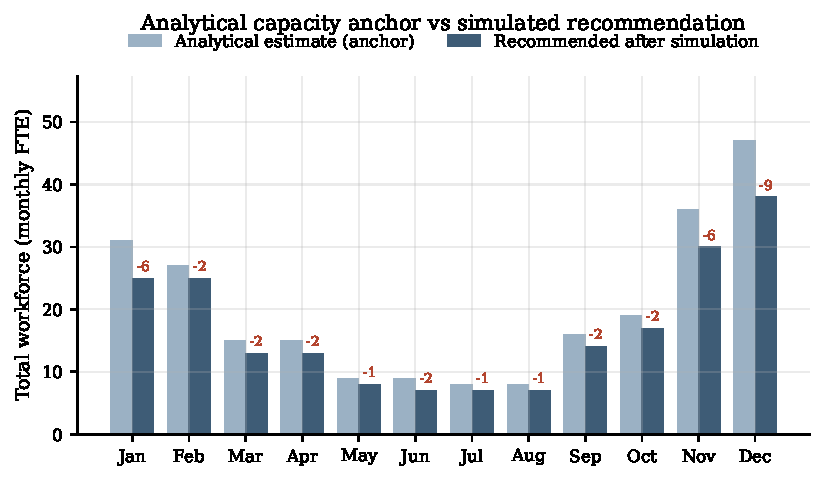
\includegraphics[width=\textwidth]{f3_analytical_vs_recommended.pdf}
\caption[Analytical estimate against simulated recommendation]{Analytical capacity anchor
against the workforce recommended after simulation. The annotation on each pair gives the
difference. The estimate exceeds the simulated recommendation in all twelve months.}
\label{fig:analytical}
\end{figure}

The magnitude is material. December's nine-FTE difference corresponds to
\(9 \times \num{2400} = \eur{21600}\) of monthly labour cost under that run's economic
assumptions. Against an analytical estimate of 47 FTE, a simulated recommendation of 38 is
\(9/47 \approx \SI{19}{\percent}\) below the estimate; expressed instead as a share of the
recommended workforce the same nine FTE are \(9/38 \approx \SI{24}{\percent}\). The first of
these --- the difference as a proportion of the analytical estimate --- is the form used
consistently throughout this thesis. Aggregated across the
peak months alone, the difference between sizing by formula and sizing by simulation is
measured in tens of thousands of euros per year.

Two mechanisms account for the gap, and they work in the same direction. First, the analytical
estimate deliberately targets \SI{85}{\percent} utilisation, which builds in a safety margin.
Second, and more interestingly, the estimate has no way of knowing that a sequencing policy can
protect the urgent class. It sizes capacity as though all orders were interchangeable, whereas
the simulated evaluation discovers that a smaller workforce combined with an urgency-aware
sequencing rule satisfies both service floors. The estimate cannot represent that substitution
between capacity and operating discipline, and consequently over-provides capacity.

\subsection{Where the over-estimation falls}
\label{sec:res-stage-gap}

Decomposing the gap by stage shows that it is not distributed evenly.
\Cref{tab:stage-gap} gives the per-stage difference between the analytical estimate and the
recommended configuration.

\begin{table}[htbp]
\centering
\caption[Per-stage difference between estimate and recommendation]{Analytical estimate against
recommended configuration, by stage. Values are picking / packing / dispatch FTE.}
\label{tab:stage-gap}
\small
\begin{tabular}{lccc}
\toprule
\textbf{Month} & \textbf{Analytical} & \textbf{Recommended} & \textbf{Difference} \\
\midrule
January   & 16 / 10 / 5 & 13 / 8 / 4 & \(-3\) / \(-2\) / \(-1\) \\
February  & 14 / 8 / 5  & 13 / 8 / 4 & \(-1\) / \(0\) / \(-1\) \\
March     & 7 / 5 / 3   & 6 / 4 / 3  & \(-1\) / \(-1\) / \(0\) \\
April     & 7 / 5 / 3   & 6 / 4 / 3  & \(-1\) / \(-1\) / \(0\) \\
May       & 4 / 3 / 2   & 3 / 3 / 2  & \(-1\) / \(0\) / \(0\) \\
June      & 4 / 3 / 2   & 3 / 2 / 2  & \(-1\) / \(-1\) / \(0\) \\
July      & 3 / 3 / 2   & 3 / 2 / 2  & \(0\) / \(-1\) / \(0\) \\
August    & 3 / 3 / 2   & 3 / 2 / 2  & \(0\) / \(-1\) / \(0\) \\
September & 8 / 5 / 3   & 7 / 4 / 3  & \(-1\) / \(-1\) / \(0\) \\
October   & 9 / 6 / 4   & 8 / 6 / 3  & \(-1\) / \(0\) / \(-1\) \\
November  & 19 / 11 / 6 & 16 / 9 / 5 & \(-3\) / \(-2\) / \(-1\) \\
December  & 26 / 14 / 7 & 22 / 11 / 5 & \(-4\) / \(-3\) / \(-2\) \\
\midrule
\textbf{Total} & & & \(\mathbf{-17}\) / \(\mathbf{-13}\) / \(\mathbf{-6}\) \\
\bottomrule
\end{tabular}
\end{table}

Summed across the year, the estimate over-provides by 17 picking FTE, 13 packing FTE and 6
dispatch FTE. In absolute terms picking absorbs the largest correction, which is unsurprising
since it is the largest stage. In \emph{relative} terms, however, packing is over-provided most
consistently: it is reduced in eight of the twelve months, including the summer months where
picking is not reduced at all.

The reason is that the analytical estimate rounds each stage up independently. A stage whose
computed requirement is only slightly above an integer receives a full additional worker, and
the smaller the stage, the larger that rounding is as a proportion of its capacity. Packing,
sitting between a large picking stage and a small dispatch stage, is most exposed to this
effect. In July and August the estimate calls for three packing FTE where two suffice --- a
third of the stage's capacity, obtained purely from rounding.

This is worth noting because it identifies a second, quite separate source of the gap. The
substitution between capacity and sequencing discipline explains the large corrections in the
peak months; independent per-stage rounding explains the persistent one-worker corrections in
the quiet ones. Both push in the same direction, and neither is visible without simulating.

\section{Sequencing policies (RQ2)}
\label{sec:res-policy}

Every comparison in this section is made under common random numbers, so the three policies face
identical order arrivals and identical service times for every order at every stage. Where two
policies are compared at the same workforce configuration, the only difference between the runs
is the order in which waiting work was selected. Differences reported below therefore reflect
the sequencing decision itself and not variation in the demand or service realisation. The
evidence that this synchronisation holds is visible in the results: at a given configuration the
three policies produce stage utilisations that agree to within a tenth of a percentage point,
which would not occur if they were drawing different service times.

Two complementary views are reported. The equal-workforce view isolates the effect of sequencing
by holding capacity constant. The minimum-feasible-workforce view
(\Cref{sec:res-min-feasible}) asks what each policy costs in capacity terms, which is the form
in which the comparison enters a budget discussion. The two answer different questions and are
kept separate throughout.

\subsection{Feasibility}

The single most decisive result concerns how often each policy can satisfy the service floors
at all. \Cref{tab:feasibility} and \Cref{fig:feasibility} report, for each month, the number of
the sixteen candidate configurations that met both floors under each policy.

\begin{table}[htbp]
\centering
\caption[Feasible configurations by month and policy]{Number of the sixteen candidate
configurations meeting both service floors, by month and policy.}
\label{tab:feasibility}
\small
\begin{tabular}{lrrr@{\hskip 2em}lrrr}
\toprule
\textbf{Month} & \textbf{FIFO} & \textbf{UF} & \textbf{RL-3} &
\textbf{Month} & \textbf{FIFO} & \textbf{UF} & \textbf{RL-3} \\
\midrule
January   & \textbf{0} & 16 & 16 & July      &  9 & 11 & 11 \\
February  & \textbf{0} & 15 & 15 & August    &  9 & 11 & 11 \\
March     & 11 & 14 & 14 & September & 11 & 16 & 16 \\
April     & 11 & 14 & 14 & October   & 14 & 16 & 16 \\
May       &  8 & 11 & 11 & November  & \textbf{0} & 16 & 16 \\
June      & 11 & 11 & 11 & December  & \textbf{0} & 15 & 16 \\
\midrule
\multicolumn{8}{l}{\textbf{Total across all 192 runs per policy:}
FIFO \textbf{84}, Urgent-First \textbf{166}, RL-3 \textbf{167}} \\
\bottomrule
\end{tabular}
\end{table}

\begin{figure}[htbp]
\centering
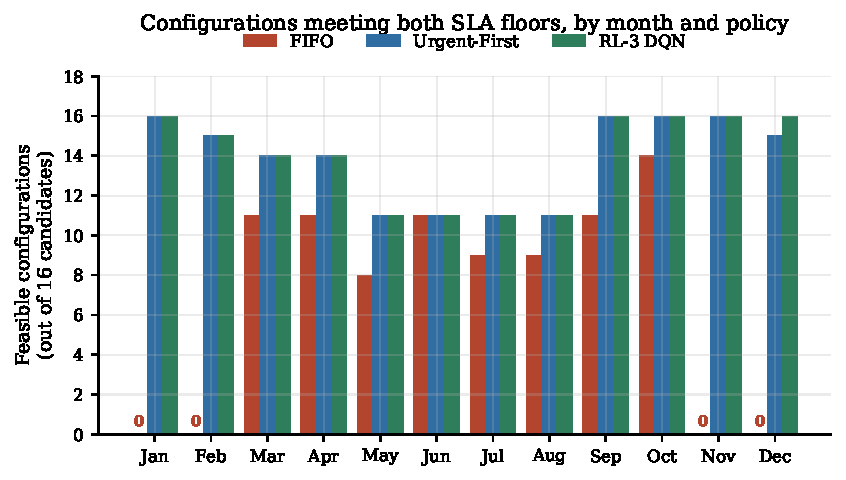
\includegraphics[width=\textwidth]{f4_feasibility_by_month.pdf}
\caption[Feasible configurations by month and policy]{Configurations meeting both service
floors, by month and policy. In the four campaign months FIFO satisfies the floors at none of
the sixteen candidates.}
\label{fig:feasibility}
\end{figure}

Two patterns stand out. First, aggregated over all 192 runs per policy, FIFO is feasible in
\num{84} while Urgent-First and RL-3 are feasible in \num{166} and \num{167} respectively ---
roughly double.

Second, and more striking, FIFO's failures are not spread evenly. Its \num{108} infeasible
configurations occur in every month of the year --- \num{44} of them across the eight
non-campaign months, so it would be wrong to say the failures fall entirely in peak --- but what
happens
\emph{only} in peak is total infeasibility. In January, February, November and December, the
four campaign months and precisely the months with the highest volume and the highest urgent
share, FIFO satisfies the service floors at \emph{none} of the sixteen candidate workforces,
whereas in every other month at least eight of the sixteen are feasible. Within the evaluated
range, adding capacity does not rescue it in those four months. The reason is one of discipline
rather than of capacity: a first-in-first-out queue gives an urgent order no precedence over the
large volume of normal orders ahead of it, and with a \SI{240}{\minute} threshold against a
\SI{1440}{\minute} one, the urgent class fails first and fails hardest. A workforce large enough
to keep every queue short would eventually satisfy both floors under FIFO too; none of the
candidates a planner would consider for these months is that large.

\subsection{The class-level trade-off}

\Cref{fig:tradeoff} plots urgent against normal service attainment for all 576 runs. The
structure of the plot is the finding. FIFO observations are dispersed down the vertical axis:
normal attainment is frequently high --- often above \SI{90}{\percent} --- while urgent
attainment falls as low as \SI{10}{\percent}. Urgent-First and RL-3 observations are compressed
into a band along the top, with urgent attainment near \SI{100}{\percent} almost everywhere,
and vary instead along the horizontal axis according to how much normal service they retain.

\begin{figure}[htbp]
\centering
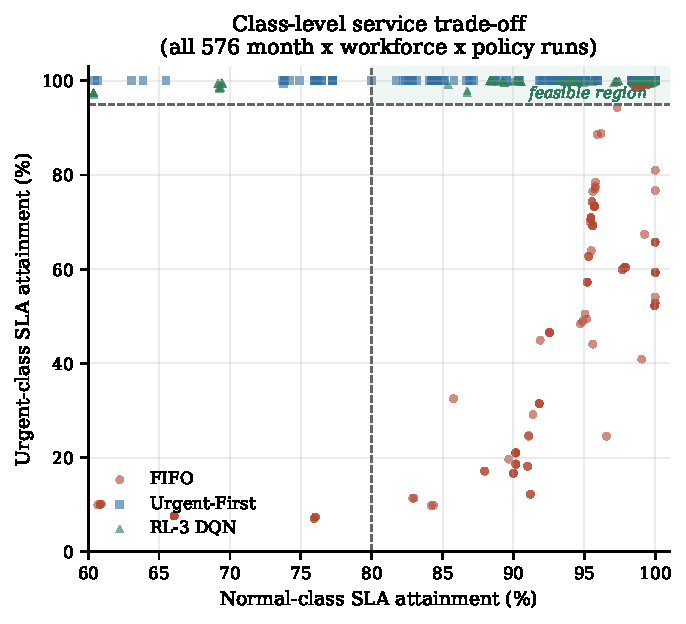
\includegraphics[width=0.82\textwidth]{f5_class_sla_tradeoff.pdf}
\caption[Class-level service trade-off]{Urgent against normal service attainment for all 576
runs. The shaded region satisfies both floors. FIFO sacrifices the urgent class; the two
urgency-aware policies differ mainly in how much normal service they retain.}
\label{fig:tradeoff}
\end{figure}

This shows that the operative question is not whether to protect the urgent class --- both
urgency-aware policies do that almost completely --- but what protecting it costs the normal
class. That is where Urgent-First and RL-3 separate, and it is the mechanism behind the
December result below.

\subsection{Three representative capacity regimes}

Aggregate counts conceal how strongly the answer depends on the capacity regime.
\Cref{tab:cases} reports three configurations chosen to span the range, and
\Cref{fig:cases} shows two of them.

\begin{table}[htbp]
\centering
\caption[Representative capacity regimes]{Three configurations spanning the capacity range.
All three policies face identical stochastic realisations under common random numbers.}
\label{tab:cases}
\small
\begin{tabular}{llrlrrrlr}
\toprule
\textbf{Month} & \textbf{Config.} & \textbf{FTE} & \textbf{Policy} &
\textbf{Urgent} & \textbf{Normal} & \textbf{Total} & \textbf{Feasible} & \textbf{Cost} \\
 & & & & \textbf{(\%)} & \textbf{(\%)} & \textbf{(\%)} & & \textbf{(EUR)} \\
\midrule
\multirow{3}{*}{October} & \multirow{3}{*}{\rgm{s753}} & \multirow{3}{*}{15}
  & FIFO & 24.5 & 91.1 & 81.0 & no  & \num{90460} \\
 & & & UF   & 100.0 & 84.2 & 86.6 & yes & \num{49635} \\
 & & & RL-3 & 99.7 & 89.4 & 90.9 & yes & \textbf{\num{45400}} \\
\midrule
\multirow{3}{*}{October} & \multirow{3}{*}{\rgm{s11\_7\_5}} & \multirow{3}{*}{23}
  & FIFO & 99.9 & 100.0 & 100.0 & yes & \num{55275} \\
 & & & UF   & 100.0 & 99.9 & 100.0 & yes & \textbf{\num{55245}} \\
 & & & RL-3 & 99.9 & 100.0 & 100.0 & yes & \num{55260} \\
\midrule
\multirow{3}{*}{December} & \multirow{3}{*}{\rgm{s22\_11\_5}} & \multirow{3}{*}{38}
  & FIFO & 19.7 & 89.7 & 71.9 & no  & \num{273140} \\
 & & & UF   & 99.3 & 73.8 & 80.2 & no  & \num{132570} \\
 & & & RL-3 & 99.2 & 85.4 & 88.9 & yes & \textbf{\num{115040}} \\
\bottomrule
\end{tabular}
\end{table}

\begin{figure}[htbp]
\centering
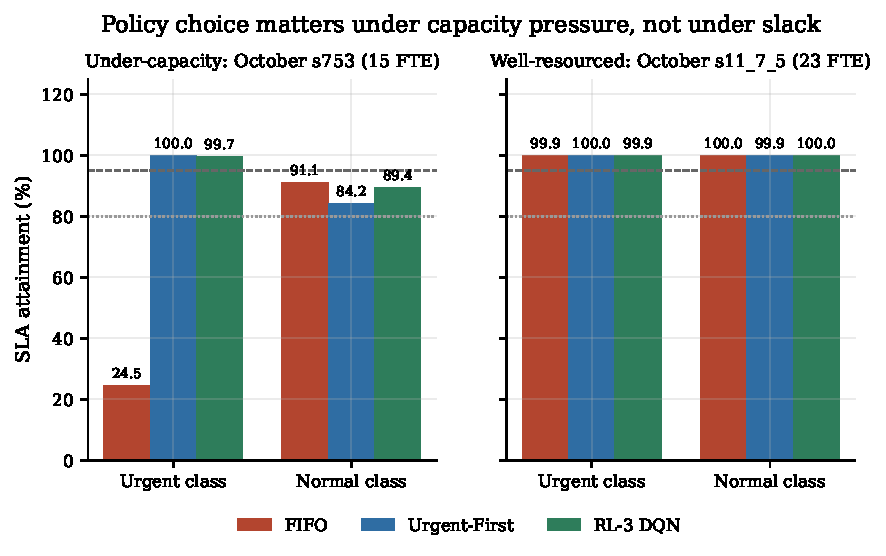
\includegraphics[width=\textwidth]{f7_representative_cases.pdf}
\caption[Policy behaviour under two capacity regimes]{Class-level attainment under two October
configurations. The dashed line marks the urgent floor (\SI{95}{\percent}) and the dotted line
the normal floor (\SI{80}{\percent}). At \rgm{s753} the policies differ dramatically; at
\rgm{s11\_7\_5} they are indistinguishable.}
\label{fig:cases}
\end{figure}

\paragraph{Under-capacity (October, \rgm{s753}, 15 FTE).} The policies diverge sharply. FIFO
delivers \SI{24.5}{\percent} urgent attainment and is infeasible. Urgent-First achieves perfect
urgent attainment but retains only \SI{84.2}{\percent} normal service. RL-3 gives up a fraction
of a percentage point of urgent attainment (\SI{99.7}{\percent}) and recovers more than five
percentage points of normal service (\SI{89.4}{\percent}), and is the cheapest of the three at
\eur{45400} against Urgent-First's \eur{49635}.

\paragraph{Well-resourced (October, \rgm{s11\_7\_5}, 23 FTE).} The policies are practically
indistinguishable. All three exceed \SI{99.9}{\percent} on both classes, and their total costs
lie within \eur{30} of one another --- a spread of \SI{0.05}{\percent}. When capacity is
sufficient, queues rarely form, so there is seldom a choice to make and the sequencing rule has
almost nothing to act on.

\paragraph{The peak (December, \rgm{s22\_11\_5}, 38 FTE).} This configuration produces the
sharpest separation observed anywhere in the study. FIFO collapses to \SI{19.7}{\percent}
urgent attainment. Urgent-First protects the urgent class successfully
(\SI{99.3}{\percent}) but, in doing so, drives normal attainment down to
\SI{73.8}{\percent} --- \emph{below the \SI{80}{\percent} floor} --- and is therefore
infeasible. RL-3 achieves essentially the same urgent attainment (\SI{99.2}{\percent}) while
holding normal service at \SI{85.4}{\percent}, and is the only feasible policy at this
configuration. It is also the cheapest, at \eur{115040} against Urgent-First's \eur{132570}, a
difference of \SI{13.2}{\percent}.

This is the strongest single result for the learned policy: at the peak month's recommended
workforce, the implemented RL-3 policy reaches a feasible outcome that the implemented
Urgent-First baseline does not reach at all, and does so at lower cost.

How far that difference can be attributed to \emph{learning} requires care, and the answer is
that it cannot be attributed to learning alone. The two implementations differ on two dimensions
at once, as \Cref{sec:urgent-first,sec:rl3} set out: RL-3 chooses which class to serve as a
function of state, and it maintains first-in-first-out order within each class; Urgent-First
applies fixed class precedence, and its within-class order follows the internal structure of a
binary heap. Both dimensions plausibly contribute to the observed normal-class gap, and this
experiment cannot decompose the contribution of each. The result reported here is a difference
between the two policies \emph{as implemented}, not an isolated estimate of what dynamic class
selection is worth. \Cref{sec:disc-uf-ordering} examines the evidence on the second mechanism,
and \Cref{sec:future-work} identifies the variant that would separate them.

\Cref{fig:cost-sla} places this configuration among December's sixteen candidates.

\begin{figure}[htbp]
\centering
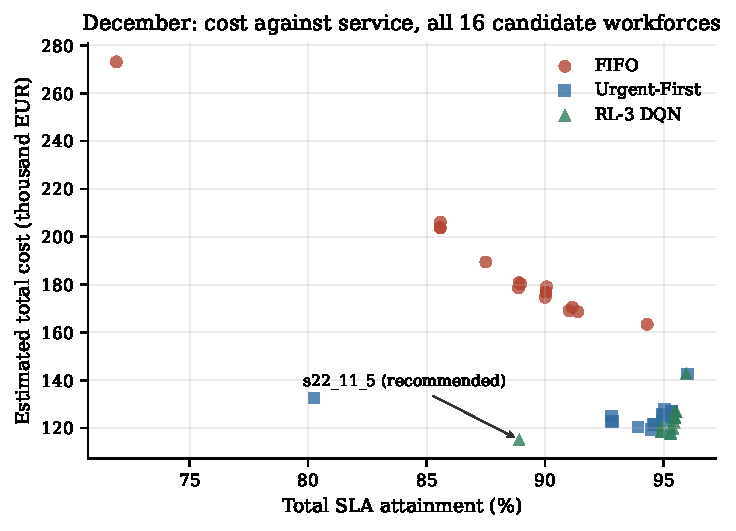
\includegraphics[width=0.85\textwidth]{f6_cost_vs_sla.pdf}
\caption[December cost against service]{Total cost against total service attainment for all
sixteen December candidates under each policy. FIFO occupies a separate, expensive and
low-service region.}
\label{fig:cost-sla}
\end{figure}

\subsection{The systematic comparison over all matched configurations}
\label{sec:res-matched}

The three configurations of \Cref{tab:cases} were chosen to illustrate. Because every (month,
workforce) pair was evaluated under all three policies on identical stochastic realisations,
the grid also supports a systematic comparison: it consists of \textbf{192 matched triples},
in each of which the only difference between the three runs is the sequencing decision.
\Cref{tab:matched} summarises the pairwise differences across all of them.

\begin{table}[htbp]
\centering
\caption[Pairwise policy differences over 192 matched configurations]{Pairwise policy
differences across all 192 matched (month, workforce) configurations. Service differences are
in percentage points; cost differences in euros under the retrospective run's assumptions.}
\label{tab:matched}
\small
\begin{tabular}{lrrrrr}
\toprule
\textbf{Comparison} & \textbf{Cheaper} & \textbf{Mean cost} & \textbf{Urgent} &
\textbf{Mean urgent} & \textbf{Mean normal} \\
 & \textbf{in} & \textbf{difference} & \textbf{better in} & \textbf{difference} &
 \textbf{difference} \\
\midrule
RL-3 vs Urgent-First & 94 / 192  & \(-575\)     & 0 / 192   & \(-0.62\) & \(-0.70\) \\
RL-3 vs FIFO         & 169 / 192 & \(-22{,}638\) & 169 / 192 & \(+32.59\) & \(-1.53\) \\
Urgent-First vs FIFO & 173 / 192 & \(-22{,}063\) & 169 / 192 & \(+33.21\) & \(-0.83\) \\
\bottomrule
\end{tabular}
\end{table}

Three observations follow, and the second and third qualify the headline results reported above.

\paragraph{Against FIFO the advantage is unambiguous.} Both urgency-aware policies improve
urgent-class attainment by more than 32 percentage points on average and reduce total cost by
roughly \eur{22000} per configuration. The cost of that improvement to the normal class is
small --- between \num{0.83} and \num{1.53} percentage points on average.

\paragraph{Against Urgent-First, RL-3 never wins on the urgent class.} In \emph{none} of the
192 configurations does RL-3 achieve higher urgent-class attainment than strict priority, and
on average it is \num{0.62} percentage points lower. This is exactly what the priority rule is
designed to guarantee, and it confirms that RL-3's contribution is not better protection of the
urgent class. Its advantage, where it exists, comes from what it gives back to the normal class.

\paragraph{The overall averages conceal a sharp regional split.} Taken over all 192
configurations, RL-3's mean normal-class difference against Urgent-First is
\emph{negative} (\num{-0.70} points) even though it is better in 125 of them --- meaning its
losses are far larger than its gains. Splitting by feasibility resolves this completely, as
\Cref{tab:matched-split} shows.

\begin{table}[htbp]
\centering
\caption[Matched comparison split by feasibility]{RL-3 against Urgent-First, split by whether
either policy produced a feasible plan at that configuration.}
\label{tab:matched-split}
\small
\begin{tabular}{lrrrr}
\toprule
\textbf{Region} & \textbf{Configs} & \textbf{Mean normal} & \textbf{Worst normal} &
\textbf{Mean cost} \\
 & & \textbf{difference (pts)} & \textbf{difference (pts)} & \textbf{difference} \\
\midrule
At least one policy feasible & 167 & \(+1.84\)  & \(-0.08\)  & \(-1{,}991\) \\
Neither policy feasible      & 25  & \(-17.69\) & \(-33.69\) & \(+8{,}880\) \\
\bottomrule
\end{tabular}
\end{table}

\textbf{Every one of RL-3's material normal-class losses occurs where neither policy produced a
feasible plan.} In the 167 configurations where a viable plan existed, RL-3's normal-class
attainment was better by \num{1.84} percentage points on average and its worst case was a loss
of \num{0.08} points --- effectively never worse. In the 25 configurations where both policies
failed, RL-3 was worse in all of them, by \num{17.69} points on average, and cost \eur{8880}
more.

Those 25 configurations are severely under-resourced: backlog shares of 27 to 35 per cent and
picking utilisation averaging \SI{93.8}{\percent}. They are found in the low-demand months at
workforces well below the recommended level --- May \rgm{s232}, for example, where FIFO attains
\SI{4.0}{\percent} urgent service, Urgent-First \SI{100}{\percent} urgent but only
\SI{57.4}{\percent} normal, and RL-3 \SI{94.1}{\percent} urgent and \SI{23.7}{\percent} normal.
None of the three is remotely acceptable. The honest reading is that RL-3 degrades less
gracefully than strict priority when capacity is grossly insufficient, but that this occurs only
in a region where no configuration would be adopted.

\subsection{Policy divergence increases with capacity pressure}
\label{sec:res-pressure-bands}

The matched design also allows the regime dependence claimed in \Cref{sec:res-policy} to be
measured rather than illustrated. Grouping the 192 configurations by picking utilisation gives
\Cref{tab:pressure-bands} and the left panel of \Cref{fig:equal-workforce}.

The statistic in the first column of that table is the \emph{absolute} cost difference
\(\lvert C_{\text{RL-3}} - C_{\text{UF}}\rvert\). It measures how far apart the two policies
land, not which of them lands lower --- a distinction that turns out to matter here, and which
the signed comparison below addresses separately.

\begin{table}[htbp]
\centering
\caption[Policy divergence by capacity-pressure band]{Divergence between RL-3 and Urgent-First
at equal workforce, grouped by picking utilisation. ``Absolute gap'' is
\(\lvert C_{\text{RL-3}} - C_{\text{UF}}\rvert\), a measure of separation; ``signed'' is
\(C_{\text{UF}} - C_{\text{RL-3}}\), positive where RL-3 is cheaper, reported separately for
configurations at which at least one policy produced a feasible plan and for those at which
neither did.}
\label{tab:pressure-bands}
\small
\setlength{\tabcolsep}{4.5pt}
\begin{tabular}{lrrrrr}
\toprule
& & \multicolumn{2}{c}{\textbf{Absolute gap (EUR)}} &
\multicolumn{2}{c}{\textbf{Mean signed gap (EUR)}} \\
\cmidrule(lr){3-4}\cmidrule(lr){5-6}
\textbf{Picking utilisation} & \textbf{Configs} & \textbf{mean} & \textbf{per 1{,}000}
& \textbf{feasible} & \textbf{neither} \\
 & & & \textbf{orders} & \textbf{exists} & \textbf{feasible} \\
\midrule
below \SI{70}{\percent}      & 33 & 537        & 55  & $-0.5$ (31)   & $-\num{8608}$ (2) \\
\SIrange{70}{80}{\percent}   & 47 & \num{1484} & 96  & $+858$ (45)   & $-\num{14925}$ (2) \\
\SIrange{80}{90}{\percent}   & 69 & \num{3004} & 106 & $+\num{2988}$ (69) & --- \\
\SIrange{90}{95}{\percent}   & 11 & \num{5563} & 283 & $+\num{4611}$ (8)  & $-\num{7987}$ (3) \\
above \SI{95}{\percent}      & 32 & \num{6320} & 545 & $+\num{3630}$ (14) & $-\num{8388}$ (18) \\
\bottomrule
\end{tabular}
\end{table}

\begin{figure}[htbp]
\centering
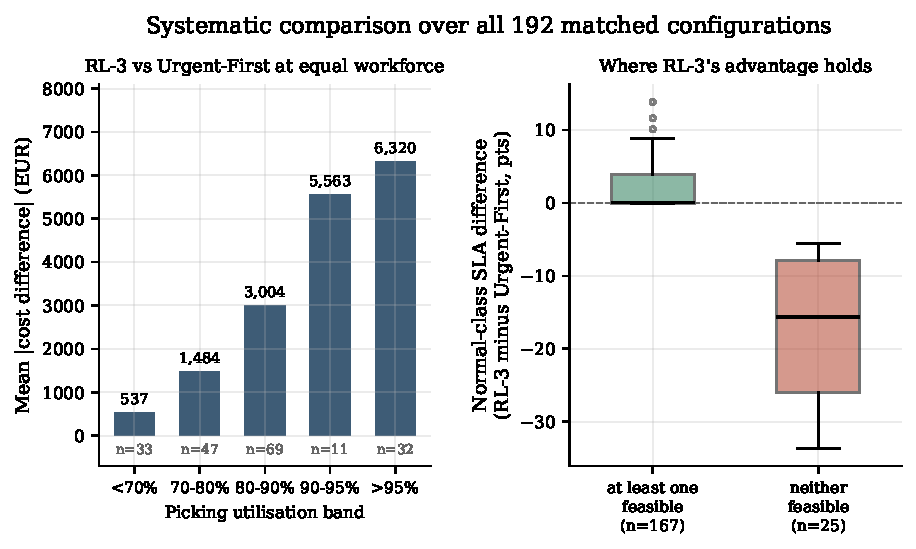
\includegraphics[width=\textwidth]{f12_equal_workforce.pdf}
\caption[Equal-workforce comparison across all configurations]{Left: the absolute cost
difference between the two urgency-aware policies grows monotonically across the observed
capacity-pressure bands. Right: RL-3's normal-class advantage over Urgent-First holds wherever a
feasible plan exists and reverses where none does.}
\label{fig:equal-workforce}
\end{figure}

The mean absolute gap rises monotonically across the five observed bands, from \eur{537} below
\SI{70}{\percent} utilisation to \eur{6320} above \SI{95}{\percent} --- a factor of nearly
\textbf{twelve}. The relationship is not driven by a handful of extreme cases: it holds for the
band means, each computed over between 11 and 69 configurations.

Two qualifications keep this statistic honest. The first is that absolute euro gaps depend on
how much there is to be late about: order volume, urgency mix and total exposure to late
penalties all vary across months, and the high-utilisation bands are populated mainly by
campaign months. Normalising per \num{1000} orders addresses that directly, and the monotone
pattern survives it --- \eur{55} per \num{1000} orders below \SI{70}{\percent} utilisation
against \eur{545} above \SI{95}{\percent}. The separation is therefore not merely a volume
artefact.

The second is that separation is not the same as advantage. The signed columns of
\Cref{tab:pressure-bands} show that where at least one policy produced a feasible plan, the
difference does favour RL-3 and does grow with pressure, from indistinguishable below
\SI{70}{\percent} to roughly \eur{3000}--\eur{4600} in the top three bands. Where neither policy
reached feasibility, the sign reverses sharply and Urgent-First is the cheaper of the two by
between \eur{8000} and \eur{15000} on average. Since \num{18} of the \num{32} configurations
above \SI{95}{\percent} utilisation fall in that second group, the growth in the absolute gap in
the top band is driven as much by the reversal as by the advantage. The right panel of
\Cref{fig:equal-workforce} shows the same split directly.

The defensible reading is therefore that \emph{divergence} between the two urgency-aware
policies increases across the observed utilisation bands, and that within the feasible region
that divergence favours RL-3. Utilisation is used here as an observed grouping variable, not as
an established cause: the bands coincide with the campaign months, with high urgent shares and
with lean configurations, and this design cannot separate those. This is the quantitative form
of the claim made from the two October configurations in \Cref{tab:cases}. Sequencing policy is
close to a free choice when capacity is comfortable and a consequential one when it is not, and
the transition is gradual rather than abrupt.

\subsection{How much workforce each policy needs to become feasible}
\label{sec:res-min-feasible}

The comparisons above hold the workforce fixed, which isolates the sequencing effect. The
complementary question is what each policy costs in \emph{capacity}: how many full-time
equivalents it requires before it satisfies both service floors at all.
\Cref{tab:min-feasible} reports the smallest feasible configuration found for each policy.

\begin{table}[htbp]
\centering
\caption[Smallest feasible workforce by policy]{Smallest total workforce at which each policy
satisfied both service floors. A dash indicates that no candidate examined was feasible. The
final column gives the range of total FTE spanned by that month's sixteen candidates.}
\label{tab:min-feasible}
\small
\begin{tabular}{lrrrl}
\toprule
\textbf{Month} & \textbf{FIFO} & \textbf{Urgent-First} & \textbf{RL-3} &
\textbf{Candidate range} \\
\midrule
January   & --- & 25 & 25 & 25--37 \\
February  & --- & 25 & 25 & 21--33 \\
March     & 13 & 13 & 13 & 11--19 \\
April     & 13 & 13 & 13 & 11--19 \\
May       &  9 &  7 &  7 & 6--12 \\
June      &  7 &  7 &  7 & 6--12 \\
July      &  7 &  6 &  6 & 5--11 \\
August    &  7 &  6 &  6 & 5--11 \\
September & 14 & 12 & 12 & 12--20 \\
October   & 17 & 15 & 15 & 15--23 \\
November  & --- & 30 & 30 & 30--42 \\
December  & --- & \textbf{45} & \textbf{38} & 38--56 \\
\bottomrule
\end{tabular}
\end{table}

Where FIFO is feasible at all, it generally requires more capacity than the urgency-aware
policies to get there --- two additional FTE in May, September and October, one in July and
August. Over most of the year the two urgency-aware policies reach feasibility at exactly the
same workforce, which reinforces the earlier finding that they are close substitutes outside the
peak.

December is the exception, and it is a substantial one. Urgent-First does not reach feasibility
until 45 FTE, whereas RL-3 reaches it at 38 --- a difference of \textbf{seven full-time
equivalents}, or \eur{16800} per month in labour cost alone under that run's assumptions. The
mechanism is the one identified in \Cref{tab:cases}: at workforces between 38 and 44 FTE,
Urgent-First protects the urgent class successfully but pushes the normal class below its
\SI{80}{\percent} floor, and the only way it can lift the normal class back above the floor is
to buy enough additional capacity that both classes are served comfortably.

Two caveats bound this table. First, the search is over sixteen candidates per month, so a
figure equal to the lower end of the candidate range --- January, February, November and
December for the urgency-aware policies --- means only that the smallest configuration
\emph{examined} was already feasible, not that a smaller one would not have been. The December
comparison is unaffected by this, since both policies were evaluated over the same range and
Urgent-First failed across the lower part of it. Second, the entries are drawn from a single
demand realisation per month, so a marginal figure could shift under a different realisation.

\subsection{Where the cost difference actually comes from}
\label{sec:res-cost-decomposition}

Because the three policies are compared at identical workforce configurations, the labour
component of total cost is by construction the same for all three. Every euro of difference
between policies is therefore attributable to the late-order penalty term.
\Cref{tab:cost-split} makes this explicit at each month's recommended configuration.

\begin{table}[htbp]
\centering
\caption[Cost decomposition at the recommended configuration]{Cost decomposition at each
month's recommended configuration. Labour cost is identical across policies because the
workforce is the same; the entire difference lies in late-order penalties.}
\label{tab:cost-split}
\small
\begin{tabular}{llrrrr}
\toprule
\textbf{Month} & \textbf{Config.} & \textbf{Labour} & \multicolumn{3}{c}{\textbf{Late-order penalties (EUR)}} \\
\cmidrule(lr){4-6}
 & & \textbf{(EUR)} & \textbf{FIFO} & \textbf{Urgent-First} & \textbf{RL-3} \\
\midrule
January   & \rgm{s13\_8\_4}  & \num{60000} & \num{99340}  & \num{24955} & \textbf{\num{14085}} \\
February  & \rgm{s13\_8\_4}  & \num{60000} & \num{54620}  & \num{11385} & \textbf{\num{7065}} \\
March     & \rgm{s643}       & \num{31200} & \num{1065}   & \textbf{\num{755}} & \num{840} \\
April     & \rgm{s643}       & \num{31200} & \num{1500}   & \textbf{\num{1240}} & \num{1260} \\
May       & \rgm{s332}       & \num{19200} & \num{2425}   & \num{2145}  & \textbf{\num{1495}} \\
June      & \rgm{s322}       & \num{16800} & \num{825}    & \num{725}   & \textbf{\num{675}} \\
July      & \rgm{s322}       & \num{16800} & \num{175}    & \num{160}   & \textbf{\num{155}} \\
August    & \rgm{s322}       & \num{16800} & \num{270}    & \textbf{\num{165}} & \num{205} \\
September & \rgm{s743}       & \num{33600} & \num{1025}   & \textbf{\num{790}} & \num{820} \\
October   & \rgm{s863}       & \num{40800} & \num{1190}   & \textbf{\num{855}} & \num{920} \\
November  & \rgm{s16\_9\_5}  & \num{72000} & \num{117390} & \num{23890} & \textbf{\num{5905}} \\
December  & \rgm{s22\_11\_5} & \num{91200} & \num{181940} & \num{41370} & \textbf{\num{23840}} \\
\bottomrule
\end{tabular}
\end{table}

The table separates the year cleanly into two regimes. In the eight low- and shoulder-season
months, penalties are small in absolute terms --- under \eur{2500} against labour costs of
\eur{16800} to \eur{40800} --- and the three policies differ by amounts that are immaterial
next to the labour bill. In the four campaign months, penalties become the dominant cost
component and the spread between policies is enormous. In November, FIFO incurs \eur{117390} of
penalties against RL-3's \eur{5905}, a reduction of \SI{95}{\percent}; even against
Urgent-First's \eur{23890}, RL-3 removes a further \SI{75}{\percent}.

The practical reading is that the sequencing policy is an instrument for controlling the
\emph{penalty} component of cost, and that this component is negligible for most of the year and
dominant in the peak. A policy decision that appears to have almost no financial consequence in
July has a five-figure consequence in November, using exactly the same workforce.

\subsection{Backlog is nearly invariant to policy}
\label{sec:res-backlog}

A further observation clarifies what sequencing does and does not achieve. At each recommended
configuration, the share of orders left unfinished at the end of the operating horizon is almost
identical across the three policies: \SI{8.59}{\percent}, \SI{8.97}{\percent} and
\SI{8.95}{\percent} in January for FIFO, Urgent-First and RL-3 respectively, and
\SI{10.42}{\percent}, \SI{11.09}{\percent} and \SI{11.10}{\percent} in December. Stage
utilisation is likewise identical to within a tenth of a percentage point.

This is the expected consequence of a non-pre-emptive discipline. Reordering a queue does not
create worker-minutes; it changes chiefly \emph{which} work is completed and in what order. The
invariance observed is close but not exact --- the January figures differ across policies by up
to \num{0.38} percentage points, and the December figures by up to \num{0.68} --- which is what
one would expect with heterogeneous service times and a finite cut-off, where ordering can move
a small number of completions across the horizon boundary. The claim supported by these
experiments is therefore the empirical one: at the configurations tested, aggregate throughput
was very nearly a property of the workforce rather than of the policy.

The finding is worth stating because it delimits what sequencing can be expected to deliver. A
policy cannot create capacity, and no sequencing rule will clear a backlog that the workforce is
too small to process. What a policy determines is the allocation of the resulting lateness
across the two service classes --- which, when those classes carry different commitments and
different penalties, is precisely the decision that governs both feasibility and cost.

\subsection{Which policy is selected}

Across the twelve months, the recommended configuration used RL-3 in seven months (January,
February, May, June, July, November and December) and Urgent-First in five (March, April,
August, September and October). FIFO was selected in none. Because a feasible configuration
existed in every month, this split is the same under the lexicographic recommendation rule and
under the descriptive lowest-cost statistic (\Cref{sec:app-rules}).

The split is not arbitrary. RL-3 is selected in the two winter peaks, the pre-Christmas ramp
and the deep summer trough, while Urgent-First is selected in the moderate shoulder months. In
the shoulder months the margins are extremely small --- August differs by \eur{10}
(\eur{16955} against \eur{16965}) --- so the practical reading is that the two urgency-aware
policies are close substitutes over much of the year, and separate decisively only when the
normal-class floor comes under pressure.

\section{Bottleneck diagnosis and the marginal FTE (RQ3)}
\label{sec:res-bottleneck}

\subsection{Where pressure concentrates}

The diagnostic identified \textbf{picking as the primary pressure location in all twelve
months}, with pressure scores between \num{0.915} and \num{0.995}
(\Cref{tab:bottleneck}, \Cref{fig:pressure}). The margin over the second-ranked stage is large:
in December, picking scores \num{0.929} against packing's \num{0.307}.

\begin{table}[htbp]
\centering
\caption[Primary bottleneck by month]{Primary pressure location by month, with the components
of its score. Picking ranks first in every month.}
\label{tab:bottleneck}
\small
\begin{tabular}{lrrrr}
\toprule
\textbf{Month} & \textbf{Pressure} & \textbf{Utilisation} & \textbf{p95 wait} &
\textbf{Late-order wait} \\
 & \textbf{score} & \textbf{(\%)} & \textbf{(min)} & \textbf{share (\%)} \\
\midrule
January   & 0.983 & 95.8 & 993.8  & 99.8 \\
February  & 0.935 & 83.8 & 849.1  & 99.9 \\
March     & 0.986 & 96.7 & 236.0  & 99.5 \\
April     & 0.986 & 96.4 & 245.7  & 100.0 \\
May       & 0.995 & 98.8 & 235.3  & 100.0 \\
June      & 0.960 & 90.1 & 104.3  & 100.0 \\
July      & 0.915 & 79.5 & 71.9   & 98.4 \\
August    & 0.918 & 80.0 & 173.5  & 98.9 \\
September & 0.952 & 88.0 & 201.8  & 99.7 \\
October   & 0.978 & 94.5 & 216.8  & 100.0 \\
November  & 0.990 & 97.5 & 1083.2 & 100.0 \\
December  & 0.930 & 90.5 & 682.2  & 83.7 \\
\bottomrule
\end{tabular}
\end{table}

\begin{figure}[htbp]
\centering
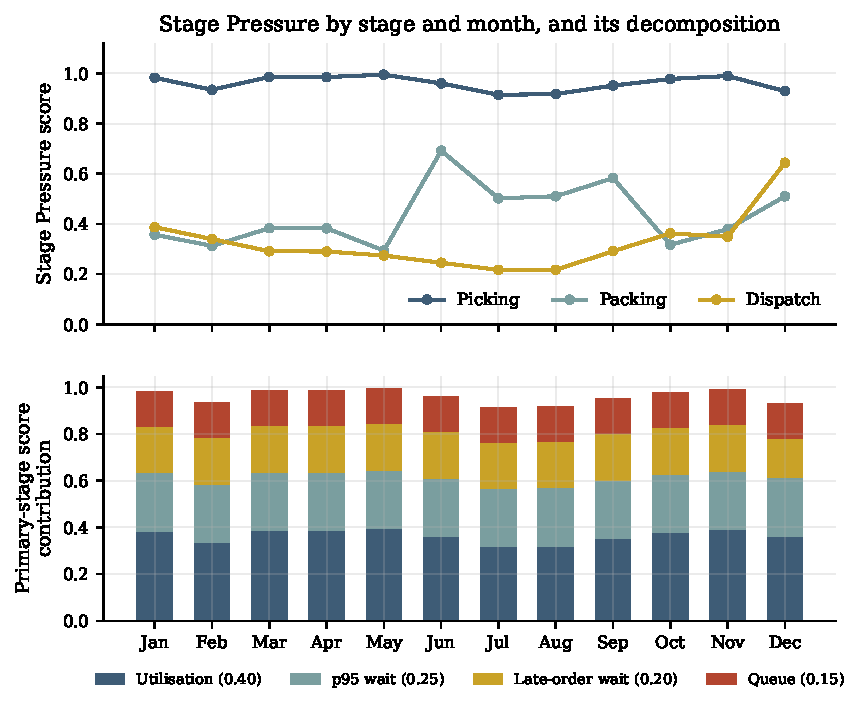
\includegraphics[width=\textwidth]{f8_stage_pressure.pdf}
\caption[Stage Pressure by stage and month]{Upper panel: pressure score of each stage by month.
Lower panel: decomposition of the primary stage's score into its four weighted components.}
\label{fig:pressure}
\end{figure}

The late-order waiting share is the most striking column: between \SI{83.7}{\percent} and
\SI{100}{\percent} of all waiting time accumulated by late orders occurs at picking. Waiting in
this system is almost entirely a picking phenomenon; packing and dispatch contribute
negligibly, even though their utilisation is often substantial. The decomposition in the lower
panel of \Cref{fig:pressure} makes the reason clear: picking saturates the relative components
(p95 wait and queue length) in every month, so its score is driven by all four signals
simultaneously.

\subsection{The most-utilised stage is not always the identified bottleneck}
\label{sec:res-util-vs-pressure}

An instructive detail is that the diagnostic does not simply select the busiest stage. In three
of the twelve months the highest-utilised stage was \emph{not} the one ranked first, as
\Cref{tab:util-vs-pressure} shows.

\begin{table}[htbp]
\centering
\caption[Utilisation against pressure ranking]{Months in which the most-utilised stage was not
ranked as the primary pressure location.}
\label{tab:util-vs-pressure}
\small
\begin{tabular}{llrrrl}
\toprule
\textbf{Month} & \textbf{Stage} & \textbf{Utilisation} & \textbf{p95 wait} &
\textbf{Late-order} & \textbf{Pressure} \\
 & & \textbf{(\%)} & \textbf{(min)} & \textbf{wait share (\%)} & \textbf{rank} \\
\midrule
\multirow{2}{*}{June}      & Picking & 90.1 & 104.3 & 100.0 & \textbf{1} \\
                           & Packing & 98.1 & 84.4  & 0.0   & 2 \\
\midrule
\multirow{2}{*}{September} & Picking & 88.0 & 201.8 & 99.7  & \textbf{1} \\
                           & Packing & 96.0 & 117.8 & 0.3   & 2 \\
\midrule
\multirow{2}{*}{December}  & Picking  & 90.5 & 682.2 & 83.7 & \textbf{1} \\
                           & Dispatch & 98.6 & 426.4 & 0.0  & 2 \\
\bottomrule
\end{tabular}
\end{table}

In June, packing ran at \SI{98.1}{\percent} utilisation against picking's \SI{90.1}{\percent},
and yet picking was ranked first with a pressure score of \num{0.960} against packing's
\num{0.692}. The reason is visible in the components: picking accounted for
\SI{100}{\percent} of the waiting time accumulated by late orders and carried both the longest
p95 wait and the largest queue, so it saturated three of the four score components, while
packing's advantage on utilisation contributed only \(0.40 \times 0.981 = 0.393\).

This behaviour follows directly from how the score is weighted, and whether it is desirable
depends on what the diagnostic is for. A stage can be almost fully occupied without generating
waiting, if work arrives at it in a steady trickle; conversely a stage can be less occupied and
still be where orders pile up, if arrivals to it are bursty. Since service failures are caused
by waiting rather than by utilisation as such, ranking by accumulated waiting is defensible for
the purpose of explaining lateness. It does mean, however, that the diagnostic answers ``where
does waiting accumulate?'' rather than ``which stage is closest to its capacity limit?'', and
those are different questions that a planner might reasonably ask on different occasions.

\subsection{A bottleneck is not a hiring instruction}

The adaptive capacity search was triggered in nine of the twelve months. The three exceptions
--- February, July and August --- are explained exactly by the trigger condition of
\Cref{sec:adaptive}: their recommended configurations were feasible and their picking
utilisation fell below the \SI{85}{\percent} threshold, at \SI{83.8}{\percent},
\SI{79.5}{\percent} and \SI{80.0}{\percent} respectively (\Cref{tab:bottleneck}). Where a plan
is comfortably feasible at moderate utilisation, the framework does not spend simulation effort
asking whether to add capacity.

In each of the nine months where it did run, the search constructed a candidate with one
additional picking worker --- the identified bottleneck --- re-simulated it under all three
policies, and compared the outcome against the incumbent. Only one stage was ever tested,
because the margin between the first- and second-ranked stages never fell below the
\num{0.05} threshold that would have prompted a second candidate; the smallest observed margin
was \num{0.268}, in June. \textbf{In all nine months the additional worker was rejected.}
\Cref{tab:adaptive} and \Cref{fig:marginal} report the comparison.

\begin{table}[htbp]
\centering
\caption[Adaptive capacity search outcomes]{Every candidate tested by the adaptive search. Each
adds one picking FTE to that month's recommended configuration.}
\label{tab:adaptive}
\small
\begin{tabular}{llrrrl}
\toprule
\textbf{Month} & \textbf{Candidate} & \textbf{Added labour} & \textbf{Penalty} &
\textbf{Net} & \textbf{Outcome} \\
 & & \textbf{(EUR)} & \textbf{saved (EUR)} & \textbf{(EUR)} & \\
\midrule
January   & \rgm{s14\_8\_4}  & \num{2400} & \num{595}  & \num{1805} & rejected \\
March     & \rgm{s743}       & \num{2400} & \num{100}  & \num{2300} & rejected \\
April     & \rgm{s743}       & \num{2400} & \num{110}  & \num{2290} & rejected \\
May       & \rgm{s432}       & \num{2400} & \num{1230} & \num{1170} & rejected \\
June      & \rgm{s422}       & \num{2400} & \num{20}   & \num{2380} & rejected \\
September & \rgm{s843}       & \num{2400} & \num{25}   & \num{2375} & rejected \\
October   & \rgm{s963}       & \num{2400} & \num{95}   & \num{2305} & rejected \\
November  & \rgm{s17\_9\_5}  & \num{2400} & \num{2025} & \num{375}  & rejected \\
December  & \rgm{s23\_11\_5} & \num{2400} & \num{20}   & \num{2380} & rejected \\
\bottomrule
\end{tabular}
\end{table}

\begin{figure}[htbp]
\centering
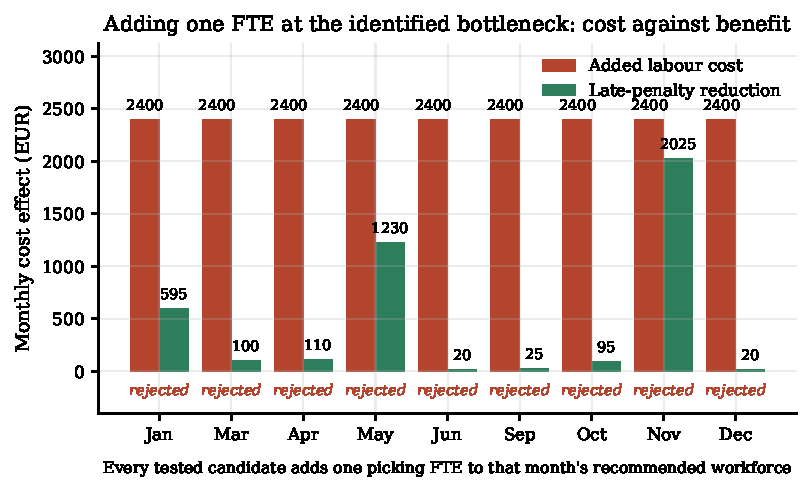
\includegraphics[width=\textwidth]{f9_marginal_fte.pdf}
\caption[The marginal FTE decision]{Cost of adding one FTE at the identified bottleneck against
the late-order penalties it avoids. The additional worker was rejected in every month tested.}
\label{fig:marginal}
\end{figure}

The economics are mostly not close. An additional FTE costs \eur{2400} per month, and in six of
the nine months it avoided less than \eur{130} of penalties --- in June and December, only
\eur{20}. Two months are closer: May recovers \eur{1230} and November \eur{2025}, the latter
within \SI{16}{\percent} of breaking even.

The December case makes the underlying arithmetic explicit. At that month's recommended
configuration, one FTE costs \eur{2400}; avoiding that cost through reduced penalties would
require preventing \num{120} late urgent orders, or \num{480} late normal orders, or about
\num{456} orders in the observed mix. The observed average penalty per late order was
EUR~5.27. The additional capacity simply does not prevent enough failures to pay for
itself, notwithstanding that picking is unambiguously the most pressured stage.

\section{Forecast-based planning (RQ4)}
\label{sec:res-future}

The forecast workflow was exercised on December. Starting from an expected volume of
\num{40800} orders and the standard uncertainty setting, it generated three stochastic
replications and evaluated candidates in two stages: all sixteen candidates screened under all
three policies on the first replication, then the four strongest validated across all three.

The recommendation was \rgm{s25\_14\_7} --- 25 picking, 14 packing and 7 dispatch FTE ---
operated under RL-3, with expected total cost \eur{158103}, urgent attainment
\SI{99.9}{\percent} and normal attainment \SI{91.9}{\percent}. The configuration met both
service floors in all three replications.

\begin{figure}[htbp]
\centering
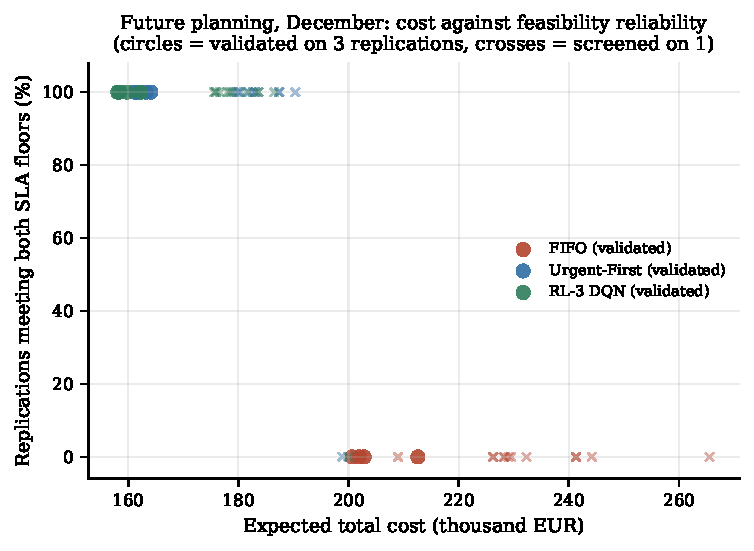
\includegraphics[width=0.85\textwidth]{f11_future_planning.pdf}
\caption[Forecast planning outcomes for December]{December candidates under forecast-based
planning: mean cost against the share of replications meeting both service floors. With three
replications that share takes only the values \(0\), \(\tfrac{1}{3}\), \(\tfrac{2}{3}\) and
\(1\). Circles were validated on three replications, crosses screened on one.}
\label{fig:future}
\end{figure}

\subsection{The screening and validation design}

The two-stage design eliminated half of the work. Stage~A screened all sixteen configurations
under all three policies on the first replication: \(16 \times 3 \times 1 = 48\) simulation
runs. Four configurations were retained as finalists, and Stage~B extended those --- and only
those --- to the two remaining replications: \(4 \times 3 \times 2 = 24\) further runs. The
first replication of the finalists is not repeated, since it was already produced during
screening. The design therefore consumed \(48 + 24 = 72\) simulation runs, against the
\(16 \times 3 \times 3 = 144\) that a full three-replication evaluation of every combination
would have required --- a reduction of exactly \SI{50}{\percent}, without changing which
configuration was ultimately recommended. Of the 48 candidate-policy combinations, 36 therefore
carry single-replication screening metrics only and 12 --- four configurations under three
policies --- carry three-replication aggregates; only the latter are eligible to become the
recommendation.

\Cref{tab:future-validated} reports the validated candidates. The pattern is consistent across
all four: FIFO is infeasible everywhere, with urgent attainment between \SI{60.8}{\percent} and
\SI{70.4}{\percent}, while both urgency-aware policies meet the floors in every replication.

\paragraph{How the three-replication statistics should be read.} Three replications is a small
sample, and the statistics computed from it must be described for what they are. The workflow
reports two summary quantities beyond the mean, and both need qualification.

The first is labelled \emph{p90 cost}. It is the sample \SI{90}{\percent} quantile of three
observations, obtained by linear interpolation between the median and the largest of them ---
four-fifths of the way towards the largest --- and it is therefore dominated by the single most
expensive replication. It is a descriptive indication of
the spread observed, not an estimate of a distributional tail: with three draws, no reliable
statement about a \SI{90}{\percent} exceedance level is available. Read as ``the worst of three
plausible December realisations, approximately'', it is informative; read as a tail-risk figure
it is not, and it is not used as one anywhere in this thesis.

The second is labelled \emph{probability of meeting the SLA targets} in the framework's
interface. It is the share of the three evaluated replications in which the configuration met
both floors, so it can only take the values \(0\), \(\tfrac{1}{3}\), \(\tfrac{2}{3}\) and
\(1\). It is a replication success rate over three trials, not an estimated probability, and no
confidence statement attaches to it. The framework additionally marks a configuration feasible
when that share is at least one half --- a majority rule rather than a requirement that all
three replications succeed. In this run the distinction has no effect on the reported results,
because every validated configuration scored either \(0\) or \(1\): the twelve validated rows
divide into four FIFO rows that failed in all three replications and eight urgency-aware rows
that succeeded in all three.

\begin{table}[htbp]
\centering
\caption[Validated December candidates]{The four configurations validated across three
replications. Costs are means across replications under the forecast run's economic assumptions;
``p90'' is the sample \SI{90}{\percent} quantile of three observations and is descriptive of the
spread, not an estimated tail. ``Feasible in all reps'' records that every one of the three
replications met both floors.}
\label{tab:future-validated}
\small
\begin{tabular}{llrrrrrl}
\toprule
\textbf{Config.} & \textbf{Policy} & \textbf{FTE} & \textbf{Urgent} & \textbf{Normal} &
\textbf{Mean cost} & \textbf{p90 cost} & \textbf{Feasible} \\
 & & & \textbf{(\%)} & \textbf{(\%)} & \textbf{(EUR)} & \textbf{(EUR)} & \textbf{in all reps} \\
\midrule
\multirow{3}{*}{\rgm{s25\_14\_7}} & FIFO & \multirow{3}{*}{46}
   & 60.8 & 94.0 & \num{212595} & \num{225353} & no \\
 & UF   & & 100.0 & 90.2 & \num{163262} & \num{172993} & yes \\
 & RL-3 & & 99.9 & 91.9 & \textbf{\num{158103}} & \num{168923} & yes \\
\midrule
\multirow{3}{*}{\rgm{s26\_14\_7}} & FIFO & \multirow{3}{*}{47}
   & 68.3 & 94.7 & \num{201963} & \num{219823} & no \\
 & UF   & & 100.0 & 91.8 & \num{161162} & \num{171617} & yes \\
 & RL-3 & & 99.9 & 92.7 & \num{158395} & \num{168414} & yes \\
\midrule
\multirow{3}{*}{\rgm{s27\_14\_7}} & FIFO & \multirow{3}{*}{48}
   & 70.1 & 95.1 & \num{200672} & \num{219850} & no \\
 & UF   & & 100.0 & 92.6 & \num{161658} & \num{172551} & yes \\
 & RL-3 & & 99.9 & 93.2 & \num{159760} & \num{169391} & yes \\
\midrule
\multirow{3}{*}{\rgm{s27\_15\_7}} & FIFO & \multirow{3}{*}{49}
   & 70.4 & 95.2 & \num{202838} & \num{222107} & no \\
 & UF   & & 100.0 & 92.7 & \num{164107} & \num{174805} & yes \\
 & RL-3 & & 99.9 & 93.3 & \num{162252} & \num{171637} & yes \\
\bottomrule
\end{tabular}
\end{table}

Two further observations follow from this table. First, the margin between the two
urgency-aware policies is much narrower here than in the retrospective December case ---
between \eur{1855} and \eur{5159}, roughly one to three per cent --- because at these larger
workforces the normal class is no longer close to its floor and there is correspondingly less
for the learned policy to recover. This is the same regime dependence observed in
\Cref{sec:res-policy}, appearing in the forecast run as well.

Second, adding capacity beyond the recommended configuration does not reduce cost. Moving from
\rgm{s25\_14\_7} to \rgm{s27\_15\_7} adds three FTE and improves normal attainment by
1.4 percentage points under RL-3, but raises expected cost by \eur{4149}. The additional
labour is not repaid by the penalties it avoids --- the same conclusion the adaptive search
reached independently in the retrospective run.

Finally, the gap between the mean and the sample p90 cost indicates the spread observed across
the three replications. For the recommended configuration under RL-3 that gap is \eur{10820},
roughly \SI{6.8}{\percent} of the mean cost; for FIFO at the same configuration it is
\eur{12758}. Subject to the caveats above, a planner can read from this both what the plan is
expected to cost and roughly how much more expensive the least favourable of three simulated
December realisations proved to be.

Two features distinguish this output from the retrospective results. First, it is
\emph{spread-aware}: alongside the mean cost, the workflow reports the observed upper end of the
three replications and the share of replications in which the floors were met, so a planner can
distinguish a configuration that succeeded in every replication from one that succeeded on
average. \Cref{fig:future} shows that this distinction is real --- FIFO candidates cluster at a
zero success rate even where their mean cost is not the highest. With three replications this is
an indication rather than a quantified reliability estimate.

Second, the policy pattern of the retrospective run reappears under an independent demand
realisation and a different economic parameter set. At the recommended configuration FIFO
achieves \SI{60.8}{\percent} urgent attainment against RL-3's \SI{99.9}{\percent}, and RL-3's
expected cost of \eur{158103} compares with FIFO's \eur{212595}. The stage-differentiated
behaviour of the learned agent is also visible here: at \rgm{s25\_14\_7} it chose the urgent
queue in \SI{26.7}{\percent} of decisions at picking, \SI{73.2}{\percent} at packing and
\SI{100}{\percent} at dispatch.

\subsection{Stage-differentiated behaviour of the learned policy}
\label{sec:res-rl-behaviour}

The forecast run records how often the learned agent chose each class at each stage, which gives
a direct view of its behaviour rather than only of its outcomes. At the recommended
configuration the urgent queue was selected in \SI{26.7}{\percent} of decisions at picking,
\SI{73.2}{\percent} at packing and \SI{100}{\percent} at dispatch.

The spread is striking because a single set of network parameters produced all three figures.
The agent is not three policies; it is one policy conditioned on, among other things, a feature
identifying which stage the decision is being taken at. It has evidently learned to apply very
different logic depending on where in the flow it is acting --- close to indifference at
picking, a strong urgent bias at packing, and absolute priority at dispatch.

A plausible reading is that the stages differ in how consequential a deferral is. An urgent
order deferred at picking still has the whole of its remaining path in which to recover, and the
picking queue is long, so the opportunity cost of serving it ahead of many normal orders is
high. At dispatch, by contrast, the order is one operation from completion and any deferral
directly translates into lateness. This is an interpretation of the observed behaviour, not a
demonstrated mechanism: nothing in this study isolates why the agent behaves this way, and it
was not designed to do so. What can be stated is that a stage-independent rule cannot express
this pattern at all, because it applies identical logic everywhere.

\subsection{Comparability between the two runs}

It must be emphasised that this run used different economic assumptions from the retrospective
run --- a late urgent order is penalised at \eur{15} rather than \eur{20}, a late normal order
at \eur{10} rather than \eur{5}, and labour costs \eur{18} per hour rather than \eur{15}. Its
monetary values are therefore not comparable with those in
\Cref{tab:recommendations,tab:cases,tab:cost-split}. Notably, the two runs weight the two
classes of failure quite differently: the retrospective run penalises an urgent failure four
times as heavily as a normal one, while the forecast run penalises it only \num{1.5} times as
heavily. A policy that sacrifices normal orders to protect urgent ones is therefore
comparatively more attractive under the retrospective assumptions than under the forecast ones.

The comparison that \emph{is} valid is the one made within each run, between candidates and
policies evaluated under a common parameter set. That the same qualitative pattern --- FIFO
infeasible, the two urgency-aware policies close, RL-3 ahead where the normal class binds ---
appears under both parameter sets is mild evidence that the pattern is not an artefact of one
particular choice of penalties.

\section{The annual view}
\label{sec:res-annual}

The configurations examined in detail above were selected because they illustrate distinct
operating regimes. To guard against the impression that the argument rests on them, this section
reports the year as a whole.

\subsection{Three seasons, three different problems}

Read across all twelve months, the results separate into three regimes that pose different
planning problems.

\paragraph{The summer trough (May to August).} Demand falls to between \num{8400} and
\num{10800} orders per month and the urgent share to \SIrange{7.9}{9.0}{\percent}. Recommended
workforces are 7 to 8 FTE, penalties at the recommended configuration are trivial (\eur{155} to
\eur{1495}, against labour costs of \eur{16800} to \eur{19200}), and the policies differ by tens
of euros. FIFO remains feasible
at 8 to 11 of the 16 candidates. In this regime the planning question is simply how far capacity
can be reduced without breaching the floors; the sequencing rule is close to irrelevant.

\paragraph{The shoulder months (March, April, September, October).} Demand runs between
\num{16800} and \num{20400} orders with urgent shares of \SIrange{12.1}{15.2}{\percent}.
Recommended workforces are 13 to 17 FTE. FIFO is now feasible at only 11 to 14 candidates and
begins to fail at the leaner configurations, while the two urgency-aware policies remain feasible
at 14 to 16. Urgent-First is selected as lowest-cost in all four of these months, and its margin
over RL-3 is small --- between \eur{20} and \eur{85}. This is the regime in which an urgency-aware
rule has become necessary but a sophisticated one has not.

\paragraph{The campaign months (January, February, November, December).} Demand rises to between
\num{26400} and \num{40800} orders with urgent shares of \SIrange{18.0}{25.4}{\percent}, and
recommended workforces to 25 to 38 FTE. FIFO is feasible at \emph{none} of the 16 candidates in
any of the four --- the only months in which that happens, and the reason the candidate range
itself, rather than any property of capacity in general, bounds the claim. Penalty costs become the dominant cost component, and the spread between
policies runs into five figures. RL-3 is selected in all four. This is the regime in which the
sequencing decision determines whether a viable plan exists at all.

\subsection{The recommendation is not a smooth function of volume}

\Cref{tab:recommendations} shows that the recommended workforce does not scale proportionally
with demand. December handles \num{4.86} times July's volume but requires \num{5.43} times the
workforce, whereas March handles \num{1.56} times May's volume with \num{1.63} times the
workforce. Two effects pull in opposite directions. Workload per order rises with volume, as
\Cref{sec:res-demand} showed, so peak months need proportionally more capacity per order ---
which is why December's ratio exceeds its volume ratio. Against that, integer rounding at three
stages is proportionally more costly in small configurations, which inflates the summer months'
workforces relative to a smooth curve and compresses the ratios between them.

The practical consequence is that a planner cannot scale a known good configuration by a demand
ratio. The recommendation for a month with twice the volume is not twice the workforce, and the
error runs in both directions depending on where in the seasonal cycle the reference month sits.

\subsection{Consistency of the qualitative findings}

Three findings hold in every month examined, without exception:

\begin{itemize}
  \item picking is the primary pressure location (12 of 12);
  \item the analytical estimate exceeds the simulated recommendation (12 of 12);
  \item where the adaptive search ran, the additional FTE was rejected (9 of 9).
\end{itemize}

\noindent Two hold with clear exceptions that are themselves explicable:

\begin{itemize}
  \item FIFO is never selected as lowest-cost (12 of 12), but it \emph{is} feasible in the
        eight non-campaign months, so it is not universally unusable --- only unusable under
        pressure;
  \item RL-3's normal-class advantage over Urgent-First holds throughout the feasible region
        (167 configurations, worst case \(-0.08\) points) and reverses entirely outside it
        (25 configurations, mean \(-17.69\) points).
\end{itemize}

\section{Summary of observations}
\label{sec:res-summary}

\begin{enumerate}
  \item Orders impose markedly different workload at the three stages
        (\(1 : 0.72 : 0.34\)), and seasonal growth concentrates on picking.
  \item The analytical capacity estimate exceeded the simulated recommendation in all twelve
        months, by up to nine FTE in December.
  \item FIFO was feasible in \num{84} of \num{192} runs against \num{166} and \num{167} for the
        two urgency-aware policies. Its infeasible configurations occur in every month, but
        \emph{complete} monthly infeasibility --- no feasible configuration among the sixteen
        --- occurs only in the four campaign months.
  \item Policy differences are large under capacity pressure and negligible under slack: at
        October \rgm{s11\_7\_5} the three policies differ in total cost by \eur{30}.
  \item At the December recommended configuration, RL-3 was the only feasible policy, at
        \SI{13.2}{\percent} lower cost than Urgent-First.
  \item Picking was the primary pressure location in all twelve months and accounted for
        \SIrange{83.7}{100}{\percent} of late orders' accumulated waiting.
  \item The adaptive search tested one additional picking FTE in nine months and rejected it in
        all nine.
  \item The forecast workflow reproduced the qualitative policy pattern under independently
        generated demand, reporting results across three replications rather than a single
        point estimate. Three replications describe the spread observed; they do not quantify
        risk.
\end{enumerate}

\chapter{Discussion}
\label{ch:discussion}

\Cref{ch:results} reported what was observed. This chapter asks what it means. It works through
the four research questions in turn (\Cref{sec:disc-capacity,sec:disc-policy,%
sec:disc-bottleneck,sec:disc-modes}), relates the findings to the literature
(\Cref{sec:disc-literature}), draws out what follows for practice
(\Cref{sec:disc-managerial}), and closes with what the study cannot support
(\Cref{sec:external-validity,sec:disc-limitations}).

\section{What simulation adds to capacity planning (RQ1)}
\label{sec:disc-capacity}

The most consistent result of this study is that the analytical capacity estimate exceeded the
simulated recommendation in every one of the twelve months, by as much as nine full-time
equivalents in December. That direction is worth dwelling on, because it is the opposite of
what one might expect.

The intuitive argument for simulating rather than calculating is that a formula \emph{under}
-estimates requirements: it ignores queueing, and queueing makes things worse. That argument is
sound as far as it goes, and it is why the analytical estimate here targets \SI{85}{\percent}
utilisation rather than \SI{100}{\percent} --- a margin motivated precisely by the
utilisation--congestion relationship that makes waiting time grow without bound as utilisation
approaches one \citep{hopp2011}. The safety margin accounts for part of the observed gap.

It does not account for all of it, and the remainder is the more interesting finding. The
analytical estimate sizes capacity as though every order were interchangeable. It has no
representation of the fact that a sequencing policy can decide \emph{which} orders wait. Once
the evaluation allows an urgency-aware discipline, a smaller workforce becomes sufficient,
because the scarce capacity is directed at the orders whose deadlines are binding. What the
simulation discovers, in other words, is a \emph{substitution between capacity and operating
discipline} — and that substitution is invisible to any formula that reasons about aggregate
workload.

This reframes the contribution of simulation to capacity planning. It is not merely a more
accurate calculator of the same quantity. It evaluates a fundamentally larger decision space,
one in which how work is ordered is a decision variable rather than a fixed background
condition. A planner using the formula alone would be choosing among workforce sizes; a planner
using the framework is choosing among (workforce, discipline) pairs, and the best pair is
cheaper than the best size.

The practical magnitude is not trivial. Nine FTE in December is roughly \SI{19}{\percent} of
the analytical estimate of 47, and even the modest one-FTE gaps in the summer months are real
money. But the direction carries a caution as well: because the framework
recommends leaner configurations than the formula, it depends more heavily on the sequencing
policy actually being implemented as modelled. A recommendation of 38 FTE operating under RL-3
is not a recommendation of 38 FTE operating under whatever discipline the floor happens to use.

\section{Sequencing policy and differentiated service (RQ2)}
\label{sec:disc-policy}

\subsection{Policy value is conditional on the capacity regime}

The headline finding on sequencing is not that one policy dominates. It is that the
\emph{magnitude} of the difference between policies depends almost entirely on how tightly
capacity is constrained.

At October's \rgm{s11\_7\_5} configuration, all three policies exceeded \SI{99.9}{\percent}
attainment on both classes and their total costs differed by \eur{30} --- five hundredths of
one per cent. At October's \rgm{s753} configuration, in the same month with the same demand,
FIFO delivered \SI{24.5}{\percent} urgent attainment while the alternatives delivered essentially
\SI{100}{\percent}. The system is the same; only the capacity is different.

The mechanism is straightforward once stated. A sequencing policy can only act when there is a
queue to choose from. When capacity is ample, queues are short and transient, decision points
are rare, and every policy makes broadly the same choices because there is usually only one
order waiting. When capacity is tight, queues are long and persistent, decision points are
continuous, and the policy determines the entire allocation of waiting across the order
population.

The consequence for practice is that ``which sequencing policy should we use?'' is the wrong
question asked in isolation. The right question is whether the operation runs close enough to
its capacity limit for the answer to matter --- and, in this study's demand profile, it does so
in roughly a third of the year.

\subsection{Why FIFO fails, and why capacity did not rescue it in the evaluated range}

FIFO's failure in the four campaign months is categorical rather than marginal: it satisfied
the service floors at none of the sixteen candidate configurations in January, February,
November or December. Elsewhere in the year its failures are partial --- \num{44} infeasible
configurations spread over the eight remaining months --- so what distinguishes the campaign
months is
that no candidate at all worked. This deserves careful interpretation, because it is tempting to
read it as ``FIFO simply needs more capacity''.

That reading is not supported by the range examined. The candidate sets in those months extend
well above the analytical estimate, and FIFO fails throughout. The reason is structural. Under FIFO an urgent
order entering the queue behind a large volume of normal orders must wait for all of them, and
its deadline is six times tighter (\SI{240}{\minute} against \SI{1440}{\minute}). Because
urgent orders are a minority of volume even in December --- roughly a quarter --- the expected
wait ahead of any urgent order is dominated by normal orders. Adding capacity shortens all
queues proportionally; it does not change the fact that the urgent order's position in the
queue bears no relation to its deadline. To satisfy a \SI{240}{\minute} threshold under FIFO,
one would need enough capacity to keep essentially \emph{every} queue short. No configuration
in the evaluated range came close, and the capacity that would be required lies far outside the
economically sensible band.

The claim this supports is bounded, and the boundary matters. FIFO is not incapable of meeting
differentiated deadlines in principle --- with a large enough workforce, queues shorten until
even the least favourably positioned urgent order clears its threshold. What the experiment
establishes is that within the sixteen workforce candidates evaluated, in each of the four
campaign months, no such configuration existed, so the shortfall could not be closed by the
capacity levers a planner would actually consider. This is a concrete instance of a point well
established in scheduling theory but easy to lose in practice: when deadlines are
differentiated, a discipline that ignores the differentiation is expensive to repair by
resourcing alone \citep{panwalkar1977}. It is cheaper to encode the commitment in the operating
rule.

\subsection{What the learned policy actually contributes}

RL-3 was the lowest-cost policy in seven of twelve months and Urgent-First in five, which on
its own would be an unremarkable split. The substantive finding is narrower and more specific.

Both urgency-aware policies protect the urgent class almost completely --- the class-level
trade-off plot shows them compressed into a narrow band near \SI{100}{\percent} urgent
attainment. They differ in what that protection costs the normal class. Strict priority, by
construction, gives the normal class whatever capacity remains after every urgent order has been
served. When the urgent share is small this is inexpensive; when it grows, the normal class
absorbs the entire shortfall.

December is where this becomes decisive. At the recommended configuration, Urgent-First achieved
\SI{99.3}{\percent} urgent attainment but drove normal attainment to \SI{73.8}{\percent},
\emph{below the \SI{80}{\percent} floor}, and was therefore infeasible. RL-3 achieved
essentially identical urgent attainment (\SI{99.2}{\percent}) while holding the normal class at
\SI{85.4}{\percent}. It was the only feasible policy at that configuration, and it was
\SI{13.2}{\percent} cheaper.

What the learned policy contributes, then, is not better urgent-class protection --- strict
priority already achieves that. It is the ability to \emph{stop} protecting the urgent class at
the point where doing so costs more than it gains. The stage-differentiated decision shares
observed in the forecast run are consistent with this: the agent chose the urgent queue in
\SI{26.7}{\percent} of picking decisions but \SI{100}{\percent} of dispatch decisions. Picking
is where the queue is long and where deferring an urgent order is cheap in slack terms; dispatch
is the last opportunity to rescue an order's deadline. A fixed rule cannot make that
distinction, because it applies the same logic everywhere.

This should not be over-read. The agent was not designed to discover that behaviour, and this
study cannot establish that it represents a general principle rather than an artefact of these
training conditions. What can be said is that a policy conditioned on stage, queue state and
remaining slack found a balance that a stage-independent rule could not, in the specific regime
where the binding constraint moved from the urgent class to the normal one.

\subsection{Where the learned policy fails, and why it matters less than it appears}
\label{sec:disc-rl-failure}

The systematic comparison in \Cref{sec:res-matched} qualifies the above in two ways that a
reader inclined to favour the learned policy should take seriously.

The first is that RL-3 achieved higher urgent-class attainment than strict priority in
\emph{none} of the 192 matched configurations. This is not a defect --- it is what a strict
priority rule guarantees by construction --- but it does bound the claim that can be made. RL-3
does not protect the urgent class better; it protects it very slightly less well, by
\num{0.62} percentage points on average, and trades that for normal-class service.

The second is more substantial. Averaged over all 192 configurations, RL-3's normal-class
attainment is \emph{worse} than Urgent-First's, because in 25 configurations it loses heavily
--- by up to 34 percentage points. Reported without qualification, that would undermine the
entire argument of \Cref{sec:res-policy}.

The qualification is that all 25 of those configurations are ones in which \emph{neither} policy
produced a feasible plan. They are severely under-resourced: backlog between 27 and 35 per cent
of the month's orders, picking utilisation averaging \SI{93.8}{\percent}. In May at
\rgm{s232}, for instance, the three policies deliver urgent attainment of \SI{4.0}{\percent},
\SI{100}{\percent} and \SI{94.1}{\percent} and normal attainment of \SI{27.3}{\percent},
\SI{57.4}{\percent} and \SI{23.7}{\percent}. No manager would deploy any of them. In the 167
configurations where at least one policy produced a viable plan, RL-3's worst normal-class
result was \num{0.08} percentage points below Urgent-First --- effectively never worse --- and
its average was \num{1.84} points better.

Two readings of this are available and they should be distinguished. The favourable reading is
that RL-3's weakness is confined to a region of the decision space that is irrelevant to
practice, so it does not detract from its usefulness where plans are actually made. The
unfavourable reading is that a learned policy degrading sharply outside the conditions where it
performs well is precisely the reliability concern raised by \citet{waubert2022}: the agent was
trained across a range of workforce configurations, and its behaviour deteriorates at the edge
of that range in a way a two-line heuristic's does not.

Both readings are defensible on this evidence, and this study cannot adjudicate between them,
because it did not test the agent under conditions systematically outside its training
distribution. What can be said is that the failure mode is identified, bounded and explicable,
which is more than an aggregate performance figure would have revealed. It also suggests a
concrete safeguard for any deployment: a learned sequencing policy should be paired with a
feasibility check on the configuration it is running under, and should not be trusted in regimes
where that check fails.

\subsection{The Urgent-First implementation and its within-class ordering}
\label{sec:disc-uf-ordering}

One implementation detail bears on how the Urgent-First results should be read. As established
in \Cref{sec:urgent-first}, the priority queue orders orders strictly by class but leaves the
sequence \emph{within} a class unspecified --- it follows the internal structure of a binary
heap, which is neither first-in-first-out nor sorted by arrival.

This is not a neutral detail for the normal class. Under a first-in-first-out discipline within
the class, normal orders would wait in a predictable order and their waiting times would be
comparatively concentrated. Under heap ordering, a normal order can be overtaken repeatedly by
later arrivals of its own class, which lengthens the \emph{tail} of the waiting distribution
without necessarily increasing its mean.

The observed waiting times show exactly that signature. At January's recommended configuration
\rgm{s13\_8\_4}, picking utilisation is identical to three decimal places across all three
policies (\num{0.958}), so any difference is attributable to ordering rather than to capacity.
Under Urgent-First the \emph{mean} picking wait is \SI{301.8}{\minute} --- \emph{lower} than
FIFO's \SI{380.4}{\minute} --- while its p95 wait is \SI{1796.9}{\minute}, more than double
FIFO's \SI{842.4}{\minute}. RL-3, whose sub-queues are first-in-first-out, sits between them at
a p95 of \SI{993.8}{\minute}. Urgent-First is therefore serving the average normal order sooner
than FIFO while leaving a minority of normal orders waiting far longer than either alternative.

Because the service-level criterion is a threshold, the tail is what matters. Part of
Urgent-First's normal-class shortfall is therefore attributable to within-class ordering rather
than to the priority rule itself. A variant implementing first-in-first-out within each class
would plausibly narrow the gap to RL-3 --- and the fact that RL-3's engine \emph{does} maintain
first-in-first-out sub-queues means the comparison is not perfectly clean on this dimension.
This is stated as a limitation rather than corrected, in keeping with the decision to document
the system as implemented. It is the single most valuable target for future work identified by
this study.

\section{Explainability and the marginal FTE (RQ3)}
\label{sec:disc-bottleneck}

\subsection{One stage dominates}

Picking was the primary pressure location in all twelve months, and the concentration is
extreme: between \SI{83.7}{\percent} and \SI{100}{\percent} of the waiting time accumulated by
late orders occurred there. Packing and dispatch contribute almost nothing to lateness, despite
often running at substantial utilisation.

This is a direct consequence of the workload structure documented in
\Cref{sec:order-heterogeneity}. Picking carries roughly three times the workload units of
dispatch per order, and seasonal growth falls disproportionately on it --- picking workload per
order rose \SI{104}{\percent} between May and December against dispatch's \SI{7}{\percent}. A
model that assumed equal workload across stages would have distributed pressure evenly and
produced a materially different, and wrong, diagnosis.

That the diagnostic identifies one stage so consistently is convenient but should not be taken
as evidence that the diagnostic is sensitive. A weighted score in which one stage dominates
every component would rank that stage first under most plausible weightings. The Stage Pressure
weights were chosen for interpretability, not calibrated, and this study does not test whether
they would discriminate correctly in a more balanced operation. The appropriate claim is that
the diagnostic identified where pressure was concentrated in these scenarios, not that it is a
validated instrument.

\subsection{Diagnosis is not prescription}

The most managerially useful result of this study is arguably the negative one. In nine months
the adaptive search tested adding one worker at the identified bottleneck, and in all nine it
rejected the addition.

The gap is usually large. An FTE costs \eur{2400} per month; in six of the nine months it
avoided less than \eur{130} of late-order penalties. December is the clearest case: picking runs
at \SI{90.5}{\percent} utilisation and accounts for \SI{83.7}{\percent} of late orders' waiting
--- an unambiguous bottleneck by any reading --- and yet the tenth picking worker prevented
\eur{20} of penalties.

The reason is that the recommended configuration has already absorbed the failures that
capacity can cheaply prevent. What remains are failures concentrated in demand bursts that a
marginal worker cannot smooth, and orders whose deadlines were never going to be met. The
marginal return on capacity at that point is close to flat, while its cost is linear.

This has a clear implication for practice: \emph{a bottleneck is a description of where pressure
is, not an instruction to add capacity there}. The two are routinely conflated, and the
conflation is expensive. The value of pairing the diagnostic with an explicit economic test is
that it separates them. The framework tells a planner where the constraint is, and then tells
them --- separately, and usually in the negative --- whether relieving it is worth paying for.

November is the instructive exception, recovering \eur{2025} against a cost of \eur{2400}. At
that margin the decision is genuinely close, and factors outside the model --- risk tolerance,
the reputational cost of missing a peak, the option value of trained capacity going into
December --- could reasonably tip it. Surfacing that a decision is close is itself useful
output.

\section{Two workflows, two kinds of answer (RQ4)}
\label{sec:disc-modes}

The retrospective and forecast workflows share an engine, a feasibility criterion and an
economic model, but they do not produce the same kind of statement, and treating their outputs
as interchangeable would be a mistake.

The retrospective workflow holds demand fixed and produces a point answer: given this demand,
this configuration would have been advised. Its uncertainty structure is essentially absent ---
one realisation per month --- which is acceptable for its purpose, because the question is
counterfactual rather than predictive. Common random numbers make the \emph{comparison between
policies} fair at a given configuration, but they do not tell us how much the recommendation
would move under a different realisation of demand. That is a genuine limitation of the
retrospective evidence in this study.

The forecast workflow treats demand as uncertain and produces a spread-aware answer: this
configuration has this mean cost across replications, cost as much as that in the least
favourable of them, and met the service floors in this share of them. The two-stage screening
and validation design is a pragmatic response to cost --- evaluating every candidate on every
replication would be wasteful when most candidates are eliminated on the first --- and it makes
the consistency of the recommendation explicit rather than implicit.

The strength of that statement should not be overstated, and the constraint is the replication
count rather than the design. Three replications support a description of the spread observed;
they do not support an estimate of a cost distribution's tail, and the share of replications
meeting the floors is a success count over three trials rather than a probability with any
precision attached. The forecast workflow as exercised here therefore demonstrates that the
framework can express scenario variation and act on it, which is what RQ4 asks; it does not
deliver calibrated reliability figures, and \Cref{sec:future-work} identifies the replication
budget and genuine forecast-error propagation as the two extensions that would.

That the December forecast run reproduced the retrospective run's qualitative policy pattern
under an independent demand realisation and a different economic parameter set is mild evidence
that the pattern is a property of the system rather than of one realisation. It is only mild
evidence: both runs share the same generator, the same service-time model and the same
structural assumptions, so agreement between them is not independent corroboration.

A final point of discipline. The two runs used different economic parameters, and no absolute
monetary comparison between them appears anywhere in this thesis. This is not pedantry: the
retrospective run penalises a late urgent order at \eur{20} and the forecast run at \eur{15},
while valuing labour at \eur{15} and \eur{18} per hour respectively. Costs from the two runs are
denominated in different assumptions and are simply not the same quantity.

\section{Relation to the literature}
\label{sec:disc-literature}

The findings connect to three strands of the literature, and the connections are not uniformly
confirmatory.

\textbf{Warehouse operations research} has concentrated overwhelmingly on the internal
efficiency of picking --- storage assignment, routing, batching and zoning
\citep{dekoster2007,gu2007,vangils2018}. That focus is well justified by the cost share of
picking, and this study's finding that picking dominates pressure in every month is consistent
with it. But the response studied here is different. Where that literature asks how to make
picking faster, this study takes the picking process as given and asks how much of it to buy
and in what order to feed it. The two are complementary: an improvement in picking productivity
would shift the capacity requirement without changing the structure of the sequencing decision.

\textbf{The call for integration} across planning problems is directly relevant.
\citet{vangils2018} argue that order-picking planning problems are usually studied in isolation
and that combining them yields better outcomes than optimising each separately, a claim
reinforced by their later analysis of real-life features \citep{vangils2019}. This study
provides evidence for an analogous claim one level up: capacity and sequencing, treated
jointly, produce a cheaper feasible plan than capacity treated alone --- which is precisely what
the systematic gap between the analytical estimate and the simulated recommendation measures.

\textbf{Scheduling and priority rules.} That priority dispatching outperforms
first-in-first-out when due dates are differentiated is long established
\citep{panwalkar1977}, and the results here are consistent with it. The finding that is
\emph{not} simply a restatement concerns the boundary of that advantage: strict priority itself
fails when protecting the priority class pushes the other class below its own floor. The
classical literature largely evaluates rules against aggregate objectives such as mean tardiness
or makespan, under which a strict priority rule looks uniformly good. Under a conjunctive
class-specific constraint it does not, and December demonstrates the failure concretely.

\textbf{What queueing theory predicted, and the model confirmed.} Two results in this study are
best read as empirical confirmations that the model behaves as theory requires, rather than as
discoveries. The first is that backlog and utilisation are almost invariant to sequencing policy
(\Cref{sec:res-backlog}). Capacity fixes the worker-minutes available in the month, and no
ordering of the queue creates more of them; the conservation properties of non-pre-emptive
priority disciplines and Little's law \citep{little1961} both express that constraint. They do
not, however, guarantee that the \emph{number} of orders finishing before a finite cut-off is
identical under every discipline: service times are heterogeneous here, so a discipline that
happens to favour shorter jobs can complete slightly more of them before the horizon. The
observed figures show exactly that residual --- backlog shares of \SI{8.59}{\percent},
\SI{8.97}{\percent} and \SI{8.95}{\percent} in January across the three policies differ, but by
fractions of a percentage point. The empirical claim, which is the one this thesis makes, is
that at the configurations tested the sequencing policies produced almost identical utilisation
and backlog, so their operative effect was the allocation of lateness between classes rather
than any material change in aggregate completion. Observing that invariance is a useful internal
validation check --- had it failed by a wide margin, something in the engine would have been
wrong.

The second is the shape of the utilisation--congestion relationship. The measured \emph{absolute}
cost difference between the two urgency-aware policies rises monotonically across the five
observed utilisation bands, by a factor of nearly twelve from below \SI{70}{\percent} to above
\SI{95}{\percent}, and by a factor of roughly ten once normalised per \num{1000} orders
(\Cref{tab:pressure-bands}). This is consistent with the non-linear growth of waiting with
utilisation \citep{hopp2011}: sequencing can only act on queues, queues barely form at low
utilisation, and their length grows sharply as utilisation approaches one. Two cautions belong
with it. The measured quantity is divergence between the policies, not RL-3's advantage; within
the feasible region the signed difference does favour RL-3 and does grow with pressure, but
where no policy reaches feasibility it reverses. And utilisation is a grouping variable here,
not a demonstrated cause --- the high bands coincide with campaign months, high urgent shares
and lean configurations, which this design cannot separate. The contribution is therefore not
the mechanism, which is textbook, but its \emph{quantification} in a specific decision context:
a planner can read from \Cref{tab:pressure-bands} roughly how much separation between the two
policies to expect at their own utilisation, and whether their operation sits in the region
where that separation favours the learned policy.

\textbf{Workload control.} The closest conceptual relative to this work outside the warehousing
literature is workload control, which manages congestion by regulating the release of work into
a shop rather than by expanding capacity \citep{thurer2012}. Both approaches treat the timing and
ordering of work as a lever operating on a fixed capacity base, and both are motivated by the
observation that this lever is cheaper than capacity. The results here support that motivation
quantitatively: in the four campaign months, changing the sequencing rule was the difference
between no viable plan at any of sixteen workforces and a viable plan at almost all of them ---
an outcome none of the capacity increases within that candidate range achieved.

The differences are equally instructive. Workload control decides \emph{when} work is released;
the policies here decide \emph{which} waiting work is served next, and release is exogenous. And
where workload control typically takes capacity as given, this framework treats capacity as the
co-equal second decision. A natural synthesis --- controlling release, sequencing and capacity
jointly --- is beyond what was studied here but follows directly from putting the two literatures
side by side.

\textbf{Learning-based control.} The use of a deep Q-network to select among sequencing
decisions places this work alongside a growing literature applying reinforcement learning to
dynamic scheduling \citep{luo2020,liu2024}. The comparison should be made carefully. That
literature typically pursues policy performance as the object of study, on benchmark instances,
against objectives such as tardiness. Here RL-3 is one of three compared components inside a
capacity-planning framework, and the interesting result is not that it performs well but
\emph{where} it does: in a narrow regime where the binding constraint shifts from one class to
the other. In most of the year it is indistinguishable from a rule that takes one line to
describe. Any assessment of whether the additional complexity is warranted must weigh that
narrowness against the cost of training, maintaining and explaining a learned policy --- and in
a setting where a manager must defend the plan, explainability is not a minor consideration.

\section{Managerial implications}
\label{sec:disc-managerial}

Five implications follow for someone responsible for a monthly fulfilment plan.

\textbf{Size capacity and discipline together.} The workforce required depends on how work is
ordered. Sizing headcount from workload ratios and then choosing an operating rule separately
over-provides capacity --- here by up to \SI{19}{\percent} of the estimate in the peak month.

\textbf{Never accept an aggregate service figure.} A configuration reporting \SI{81}{\percent}
overall attainment delivered \SI{24.5}{\percent} to its urgent customers. Where commitments are
differentiated, they must be measured and constrained separately.

\textbf{Know whether you are in the regime where sequencing matters.} If the operation runs
comfortably below capacity, the operating rule is close to irrelevant and effort is better spent
elsewhere. If it runs near capacity in peak months --- as most seasonal fulfilment operations do
--- the rule determines whether the commitments can be met at all.

\textbf{Do not treat a bottleneck as a hiring case.} The constraining stage is where to look,
not automatically where to spend. In nine of nine tests here, the additional worker at the
identified bottleneck did not pay for itself. Ask what it would prevent, and price that.

\textbf{Plan peaks across scenarios, not on a single one.} For a forecast month, a mean cost is
less useful than the share of plausible demand realisations in which the plan holds. A
configuration that succeeds on average but fails in a third of the scenarios tested is not a
plan. Establishing that share with any precision needs considerably more than the three
replications used here.

\subsection{Using the pressure bands as a screening test}

One result is directly portable to an operation that has not built this framework.
\Cref{tab:pressure-bands} relates how far apart the two urgency-aware policies land to a
quantity most warehouses already measure: utilisation at the constraining stage. Below
\SI{70}{\percent} the mean absolute difference between them was \eur{537} per month; above
\SI{95}{\percent} it was \eur{6320}. The association is observed, not established as causal,
and the direction of the difference depends on whether a feasible plan exists at all.

A manager can therefore use their own utilisation figure as a cheap screening test for whether
this kind of analysis is worth commissioning at all. If the constraining stage runs comfortably
below \SI{80}{\percent} through the year, the evidence here suggests the sequencing rule is
close to a free choice and effort is better directed elsewhere --- at demand shaping, at
process improvement, or at the storage and routing decisions that the order-picking literature
addresses \citep{petersen2004}. If it runs above \SI{90}{\percent} in the peak months, as
seasonal fulfilment operations typically do, the operating discipline is likely to be worth more
than its analysis costs.

The threshold is specific to this model and this demand profile, and should be treated as an
order-of-magnitude guide rather than a calibrated rule. What is transferable is the shape of the
relationship, which follows from queueing behaviour rather than from anything peculiar to the
implementation.

\subsection{What the framework does not tell a manager}

It is worth being explicit about the questions a planner might reasonably bring to this
framework and not get an answer to, since a decision-support tool that is unclear about its own
boundaries invites misuse.

It does not say whether the recommended capacity can be \emph{staffed}. A recommendation of 22
picking FTE says nothing about whether 22 months of picking labour can be arranged into a legal,
workable shift pattern given the operation's contracts, absence rates and recruitment lead
times. That translation is a separate problem, and a configuration this framework considers
cheapest may be one the operation cannot actually roster.

It does not say whether the service thresholds are the right ones. The framework takes
\SI{240}{\minute} and \SI{1440}{\minute}, and the \SI{95}{\percent} and \SI{80}{\percent}
attainment floors, as given. Whether those commitments are commercially sensible --- whether the
urgent tier is priced to cover the capacity it requires --- is a question the model can inform
by costing alternatives, but cannot answer.

It does not say what happens outside the month. The finite horizon makes backlog visible but
does not carry it forward: December's unfinished orders do not become January's arrivals.
For an operation with sustained overload across consecutive months, that omission would
understate the problem.

And it does not detect a wrong demand forecast. The forecast workflow evaluates robustness
across realisations \emph{consistent with the volume assumption supplied to it}. If that
assumption is wrong, every candidate is evaluated against the wrong month and the reported
reliability figures are correspondingly misleading.

\section{External validity}
\label{sec:external-validity}

The framework as it stands is an academic prototype, and the distance between it and
operational deployment should not be understated.

Deployment would require, at minimum: service-time distributions fitted to observed handling
data rather than assumed; economic parameters calibrated to the operation's actual labour costs
and contractual penalties; service thresholds expressed against the operation's real calendar,
shift pattern and carrier cut-offs rather than an abstracted operating clock; a demand forecast
with a validated error structure, since the forecast workflow's output is only as good as the
volume assumption entering it; and a translation layer converting monthly FTE recommendations
into feasible rosters, which may itself be infeasible for a configuration the model considers
optimal.

Beyond calibration, external validation would require comparing the model's recommendations
against outcomes in a real operation over multiple planning cycles --- something no part of this
study attempts. Until that is done, the appropriate claim is that the framework is a coherent
instrument for comparing configurations under stated assumptions, not that it predicts the
performance of any particular warehouse.

\section{Limitations}
\label{sec:disc-limitations}

The methodological limitations were stated in \Cref{sec:method-limitations}. Four bear
repeating because they bound the interpretation of the results specifically.

\textbf{The evidence is synthetic.} Every quantitative finding is a property of a model
operating on generated data. The patterns are internally consistent and mechanistically
explicable, but none is an empirical observation about a real warehouse.

\textbf{The two engines differ in within-class mechanics.} RL-3 maintains first-in-first-out
sub-queues; the Urgent-First baseline does not. Part of the observed gap between them in
normal-class attainment is plausibly attributable to that difference rather than to the decision
rule, and this study cannot separate the two effects.

\textbf{Retrospective results rest on one realisation per month.} No confidence interval
accompanies any retrospective recommendation. A different demand realisation could shift a
marginal month's recommended configuration, and the near-ties observed in the shoulder months
--- August differed by \eur{10} --- are well within the range where this matters.

\textbf{The learned policy cannot be regenerated.} The trained network weights are not retained
in the repository. The persisted evaluation outputs are available and every RL-3 result reported
here derives from them, but exact regeneration requires the checkpoint, which was not available
in the environment used for final thesis preparation; retraining from the recorded configuration
would produce a different policy rather than the same one. The results are internally consistent
and were generated by the documented pipeline, but no claim of end-to-end reproducibility of the
RL-3 results from the distributed artefacts is made anywhere in this thesis. This is a genuine
weakness affecting one of the three compared policies, and it is recorded as such rather than
minimised.

\textbf{The state representation saturates at peak.} The learned policy's capacity and
queue-length features are clipped, and at December's candidate workforces the picking-capacity
feature and, during congestion, the picking queue-length feature both sit at their ceiling
(\Cref{sec:app-saturation}). The agent therefore had reduced resolution on exactly the
configurations where the sequencing decision mattered most. It nevertheless produced feasible
lower-cost outcomes there, so this bounds the representation rather than invalidating the
result, but it means the reported behaviour should not be extrapolated to capacities well beyond
the normalising constants.

\chapter{Conclusions, Contributions and Implications}
\label{ch:conclusions}

This chapter answers the four research questions directly, states the contributions, sets out
the implications for practice and research, and identifies future work. No new evidence or
references are introduced.

\section{Answers to the research questions}
\label{sec:answers}

\subsection*{RQ1 --- How can discrete-event simulation support monthly workforce-capacity
planning under heterogeneous warehouse demand, and what does it add over an analytical capacity
estimate alone?}

Discrete-event simulation supports the monthly capacity decision by evaluating a bounded set of
workforce candidates against the class-specific service commitments that actually bind, taking
account of queueing, arrival burstiness, stage-differentiated workload and the sequencing rule
in force. The analytical estimate retains a role as a cheap anchor that places the search in the
right region, but it is not the answer.

What simulation adds proved to be more than accuracy. In all twelve months studied, the
simulated recommendation was \emph{smaller} than the analytical estimate --- by up to nine
full-time equivalents in December, where the recommended 38 FTE lay roughly \SI{19}{\percent}
below the estimate of 47. Part of that gap is the deliberate utilisation margin built into the
formula. The remainder arises
because the formula cannot represent a substitution that the simulation discovers: directing
scarce capacity at the orders whose deadlines bind allows a smaller workforce to satisfy the
same commitments. Simulation therefore does not merely compute the same quantity more
carefully; it evaluates a larger decision space in which the operating discipline is a decision
variable rather than a fixed background condition.

\subsection*{RQ2 --- How do alternative sequencing policies affect differentiated service-level
attainment and operating cost?}

The effect is large, and it is conditional on the capacity regime.

Aggregated over 192 runs per policy, FIFO satisfied both service floors in \num{84} while
Urgent-First and RL-3 satisfied them in \num{166} and \num{167}. Its \num{108} infeasible
configurations are spread across all twelve months; what is confined to the four campaign months
is \emph{complete} monthly infeasibility. In January, February, November and
December, FIFO met both floors at \emph{none} of the sixteen candidate configurations, while in
every other month at least eight of the sixteen were feasible. Within the evaluated workforce
range, then, additional capacity did not make FIFO feasible in the campaign months. This is a
statement about the candidate set rather than a law: a sufficiently large workforce would
eventually satisfy both floors under any work-conserving discipline. What the experiment shows
is that the capacity required to do so under FIFO lies beyond the range a planner would
plausibly consider, because an urgent order's queue position bears no relation to its
deadline.

Between the two urgency-aware policies the difference is narrower and regime-dependent. Both
protect the urgent class almost completely; they differ in what that protection costs the
normal class. Where capacity is ample the three policies are practically indistinguishable ---
at October's \rgm{s11\_7\_5} they differed in total cost by \eur{30}. Where the normal-class
floor comes under pressure they separate decisively: at December's recommended configuration,
strict priority drove normal attainment to \SI{73.8}{\percent}, below its floor, and was
infeasible, while the learned policy held it at \SI{85.4}{\percent} at equivalent urgent
attainment and \SI{13.2}{\percent} lower cost.

The systematic comparison over all 192 matched configurations quantifies this regime
dependence rather than illustrating it. Grouped by utilisation at the constraining stage, the
mean cost difference between the two urgency-aware policies rises monotonically from
\eur{537} below \SI{70}{\percent} to \eur{6320} above \SI{95}{\percent} --- a factor of nearly
twelve. The value of the sequencing decision is therefore not a fixed quantity to be estimated
once, but a function of how hard the operation is being run.

The contribution of the learned policy is therefore specific: not better protection of the
urgent class --- which strict priority already achieves, and which RL-3 matched or bettered in
none of the 192 configurations --- but a better outcome for the normal class where protecting
the urgent class becomes counter-productive. That difference is a difference between the two
policies \emph{as implemented}. They differ both in how the serving class is chosen and in how
orders are ordered within a class, and this design cannot decompose the observed gap into those
two effects; the experiment establishes a difference, not a causal estimate of the value of
learning on its own. That advantage is narrow across the year, and it is bounded in a way that
must be reported alongside it: in the 25 configurations where neither policy produced a feasible
plan, the learned policy was worse than strict priority in every one, by nearly 18 percentage
points of normal-class service on average. Its advantage holds where viable plans exist and
reverses where they do not. This study does not establish that either behaviour generalises
beyond the conditions examined.

\subsection*{RQ3 --- How can stage-level bottleneck diagnostics and adaptive capacity evaluation
improve the explainability and economic interpretation of workforce recommendations?}

The diagnostic locates pressure and decomposes the judgement, so that a recommendation arrives
with a reason attached. In this study picking was identified as the primary pressure location in
all twelve months, accounting for between \SI{83.7}{\percent} and \SI{100}{\percent} of the
waiting time accumulated by late orders --- a concentration traceable to the stage-differentiated
workload structure, in which picking carries roughly three times the workload units of dispatch
per order.

The more consequential result concerns what follows from a diagnosis. Pairing the diagnostic
with an explicit economic test showed that identifying a bottleneck does \emph{not} imply that
capacity should be added there. In nine months the framework tested one additional worker at the
identified bottleneck and rejected it in all nine: an FTE costing \eur{2400} per month avoided
less than \eur{130} of penalties in six of them. The recommended configuration has already
absorbed the failures capacity can cheaply prevent, leaving a flat marginal return against a
linear marginal cost.

Explainability is improved on both counts --- the planner learns where the constraint is and,
separately, whether relieving it is worth paying for --- and the second answer is frequently the
opposite of what the first would suggest.

\subsection*{RQ4 --- How can the same simulation framework support both retrospective and
forecast-based planning, and how do their uncertainty structures differ?}

A single engine, feasibility criterion and economic model serve both workflows; they differ only
in how the order stream is obtained. The retrospective workflow replays an order-level history
and answers a counterfactual question, producing a point recommendation per month. The forecast
workflow transforms an aggregate demand assumption into freshly generated, replicated stochastic
order streams and answers a prospective question, producing a spread-aware recommendation ---
mean cost, the cost observed in the least favourable replication, and the share of replications
meeting the service floors --- refined through a screening and validation design that consumed
72 simulation runs against the 144 an exhaustive three-replication evaluation would have needed.
With three replications those figures describe the spread observed rather than estimating a
distribution.

The uncertainty structures are genuinely different and their outputs are not interchangeable.
The retrospective evidence in this study rests on one realisation per month and therefore
carries no replication-based uncertainty estimate; common random numbers make the comparison
between policies fair at a given configuration but say nothing about how the recommendation
would move under different demand. The forecast evidence expresses scenario variation, but rests
on three replications of a single month, so it describes the spread observed rather than
quantifying reliability. That the December forecast run reproduced the retrospective policy pattern under
an independent demand realisation is mild supporting evidence, weakened by the fact that both
runs share the same generator and structural assumptions.

\section{Contributions}
\label{sec:conclusions-contributions}

\textbf{Methodological.} The thesis demonstrates a design in which simulated physical capacity
and economically paid capacity are the same quantity by construction, removing a discrepancy
that would otherwise make every capacity recommendation optimistic; a finite-horizon monthly
formulation that retains unfinished work as explicit backlog instead of allowing unlimited
post-period processing to conceal insufficient capacity; a conjunctive class-specific
feasibility criterion in place of aggregate service attainment; and a three-way policy
comparison under common random numbers in which a learned policy faces exactly the stochastic
realisations that the transparent heuristics face.

\textbf{Practical.} It delivers a workflow that converts either an order-level history or an
aggregate forecast into a recommendation a manager can act on and interrogate: workforce per
stage, sequencing policy, expected cost, class-level attainment, a named pressure location with
its decomposition, and an explicit economic test of the marginal full-time equivalent.

\textbf{Empirical.} It provides evidence that the value of sequencing policy is
capacity-regime dependent --- negligible under slack, decisive under pressure --- and that a
diagnosed bottleneck is routinely not an economically justified place to add capacity. Both
findings run against common intuition and both are directly actionable.

The thesis explicitly does not contribute a new learning algorithm, a globally optimal capacity
solution, or a model validated against industrial data.

\section{Implications}
\label{sec:implications}

\textbf{For practitioners.} Capacity and operating discipline should be sized together, since
the workforce required depends on how work is ordered. Differentiated commitments must be
measured and constrained separately, because aggregate attainment conceals minority-class
failure --- one configuration in this study reported \SI{81}{\percent} overall attainment while
delivering \SI{24.5}{\percent} to urgent customers. Effort spent refining the sequencing rule is
wasted unless the operation runs near its capacity limit, and is essential when it does. A
bottleneck should be treated as a place to investigate rather than a case for hiring. Peak
months should be planned on how consistently a configuration holds across plausible demand, not on
its expected performance.

\textbf{For research.} The result that strict priority can fail a conjunctive class-specific
constraint --- by protecting one class into the failure of the other --- suggests that
evaluating dispatching rules against aggregate objectives such as mean tardiness may understate
the differences that matter when service commitments are contractual and class-specific.
Similarly, the narrowness of the regime in which the learned policy outperformed a one-line
heuristic argues for reporting \emph{where} a learned controller helps rather than whether it
wins on average.

\textbf{For methodology.} The consistent, one-directional gap between the analytical estimate
and the simulated recommendation is a caution against using workload-ratio sizing as anything
more than a starting point when service commitments are differentiated.

\section{Future work}
\label{sec:future-work}

Several directions follow from the limitations of this study, ordered by how directly they
address them.

\textbf{Resolve the within-class ordering asymmetry.} The most valuable single extension would
be an Urgent-First variant maintaining first-in-first-out order within each class, compared
against the current implementation and against RL-3. This would separate the effect of the
priority rule from the effect of within-class ordering, and would establish how much of the
learned policy's advantage survives a fairer baseline.

\textbf{Replicate the retrospective workflow.} Running each month across multiple seeds would
attach uncertainty estimates to the monthly recommendations and establish whether the
near-ties observed in the shoulder months are stable.

\textbf{Calibrate empirically.} Fitting service-time distributions to observed handling data,
and economic parameters to real labour costs and contractual penalties, is the precondition for
any predictive claim.

\textbf{Model shifts explicitly.} Translating monthly FTE into rosters, with shift patterns,
breaks and absence, would close the gap between what the framework recommends and what an
operation can implement.

\textbf{Extend the action space.} The learned policy currently chooses between two classes at
one stage. Richer formulations --- allocating workers across stages, or choosing among more
than two queues --- would test whether the approach scales beyond a binary decision.

\textbf{Sensitivity of the bottleneck diagnostic.} Because one stage dominated in every month
here, the diagnostic's ability to discriminate was never tested. Applying it to a deliberately
balanced operation would establish whether the chosen weights matter.

\textbf{Richer scenario generation and forecast uncertainty.} Propagating genuine forecast error
into the scenario generator, rather than a configured uncertainty level, would make the forecast
workflow's reliability estimates meaningful as predictions rather than as internal consistency
checks.

\section{Closing remarks}
\label{sec:closing}

The question this thesis set out to address was how discrete-event simulation can support the
joint monthly decision of how much labour capacity to deploy and in what order to release work,
under demand that is heterogeneous and service commitments that are differentiated.

The answer that emerges is that the two decisions are not separable, and that treating them as
separable is expensive in a specific and measurable way. Sizing capacity from workload ratios
over-provided by up to nine full-time equivalents in December --- the simulated recommendation
lay approximately nineteen per cent below the analytical estimate --- because the formula could
not represent the fact that a sequencing rule decides which orders wait. Conversely, the value of a sequencing rule proved
almost entirely conditional on how tightly capacity was constrained: irrelevant under slack,
and in the peak season the difference between a viable plan and no viable plan at any workforce
examined.

Two further findings are worth carrying away because they cut against expectation. A stage can
be unambiguously the bottleneck --- saturated, and responsible for almost all the waiting that
late orders accumulate --- and still be the wrong place to add a worker, because the failures
that remain are not the kind that capacity prevents. And a learned policy can be genuinely
valuable in a narrow regime while being indistinguishable, for most of the year, from a rule
that takes one line to state. Reporting where a method helps, rather than whether it wins, seems
to the author the more useful form of both results.

None of this has been validated against a real warehouse, and the thesis is careful not to
claim otherwise. What it offers is an internally coherent instrument for comparing plans under
assumptions that are stated explicitly, together with evidence about the structure of the
problem that a practitioner could test against their own operation.


%==============================================================================
%  REFERENCES
%==============================================================================
\cleardoublepage
\phantomsection\addcontentsline{toc}{chapter}{References}
\bibliography{references}

%==============================================================================
%  APPENDICES
%==============================================================================
\cleardoublepage
\appendix
\chapter{Data Schema and Generation}
\label{app:A}

\section{Order record schema}

Each order in the dataset consumed by the retrospective workflow carries the fields in
\Cref{tab:schema}. The three workload-unit fields are derived at generation time from the item
count and the product attributes, using \Cref{eq:workload-units}.

\begin{table}[htbp]
\centering
\caption[Order record schema]{Fields of an order record.}
\label{tab:schema}
\small
\begin{tabularx}{\textwidth}{llX}
\toprule
\textbf{Field} & \textbf{Type} & \textbf{Meaning} \\
\midrule
\code{order\_id}         & integer & Unique identifier, assigned in arrival order \\
\code{arrival\_time}     & timestamp & Calendar arrival time \\
\code{month}             & integer & Calendar month, 1--12 \\
\code{weekday}           & string & Day of week of arrival \\
\code{hour}              & integer & Hour of day of arrival \\
\code{order\_type}       & string & \code{urgent} or \code{normal} \\
\code{sla\_minutes}      & integer & System-time SLA threshold: 240 or \num{1440} \\
\code{num\_items}        & integer & Number of items in the order \\
\code{product\_class}    & string & Legacy A/B/C classification \\
\code{product\_family}   & string & \code{standard}, \code{fragile} or \code{bulky} \\
\code{complexity\_level} & string & \code{low}, \code{medium} or \code{high} \\
\code{picking\_units}    & float & Derived workload units at picking \\
\code{packing\_units}    & float & Derived workload units at packing \\
\code{dispatch\_units}   & float & Derived workload units at dispatch \\
\code{scenario}          & string & Scenario tag; \code{seasonal\_base} throughout \\
\bottomrule
\end{tabularx}
\end{table}

\section{Generation parameters}

\Cref{tab:generation} gives the monthly parameters driving generation. Order counts follow
directly from the annual share applied to a total of \num{240000} orders.

\begin{table}[htbp]
\centering
\caption[Monthly generation parameters]{Monthly demand generation parameters.}
\label{tab:generation}
\small
\begin{tabular}{lrrrr}
\toprule
\textbf{Month} & \textbf{Annual share} & \textbf{Orders} & \textbf{Urgent share} &
\textbf{Mean items} \\
\midrule
January   & 0.130 & \num{31200} & 0.20 & 3.6 \\
February  & 0.110 & \num{26400} & 0.18 & 3.6 \\
March     & 0.070 & \num{16800} & 0.12 & 2.8 \\
April     & 0.070 & \num{16800} & 0.12 & 2.8 \\
May       & 0.045 & \num{10800} & 0.09 & 2.2 \\
June      & 0.040 & \num{9600}  & 0.09 & 2.2 \\
July      & 0.035 & \num{8400}  & 0.08 & 2.2 \\
August    & 0.035 & \num{8400}  & 0.08 & 2.2 \\
September & 0.070 & \num{16800} & 0.12 & 3.0 \\
October   & 0.085 & \num{20400} & 0.15 & 3.0 \\
November  & 0.140 & \num{33600} & 0.22 & 4.0 \\
December  & 0.170 & \num{40800} & 0.25 & 4.4 \\
\midrule
\textbf{Total} & 1.000 & \num{240000} & & \\
\bottomrule
\end{tabular}
\end{table}

Item counts are drawn from a lognormal distribution around the monthly mean with
\(\ln\sigma = 0.5\), bounded to \([1, 12]\) items.

Product family and complexity distributions differ by urgency class but not by month:

\begin{center}
\small
\begin{tabular}{llrrr}
\toprule
\textbf{Attribute} & \textbf{Class} & \multicolumn{3}{c}{\textbf{Probabilities}} \\
\midrule
\multirow{2}{*}{Family} & & standard & fragile & bulky \\
 & normal & 0.65 & 0.20 & 0.15 \\
 & urgent & 0.45 & 0.35 & 0.20 \\
\midrule
\multirow{2}{*}{Complexity} & & low & medium & high \\
 & normal & 0.50 & 0.35 & 0.15 \\
 & urgent & 0.25 & 0.45 & 0.30 \\
\bottomrule
\end{tabular}
\end{center}

Urgent orders are therefore systematically more demanding: they are more likely to be fragile
and more likely to be of high complexity, which compounds the difficulty of meeting their
tighter deadline.

\section{Arrival pattern}

Within a month, arrivals follow a day-weight pattern with burst days --- roughly
\SI{15}{\percent} of days in the four campaign months (January, February, November, December)
carry three times the average day weight --- and an intraday profile weighted towards working
hours. This structure is preserved through the operating-time compression of
\Cref{eq:compression}, which rescales positions within the month without altering their relative
spacing.

\section{Provenance statement}
\label{sec:app-provenance}

The dataset used for the retrospective experiments comprises \num{240000} orders spanning
1~January to 31~December of the modelled year, with an overall urgent share of
\SI{17.2}{\percent}. Every record carries the scenario tag \code{seasonal\_base}, and monthly
counts reproduce the configured annual shares exactly.

These data are \textbf{synthetic}. They were generated for this study and do not derive from any
real warehouse, customer or company. The framework is capable of consuming a real order-level
history in the same schema, and that capability is part of its design; the evidence reported in
this thesis does not exercise it.

The forecast experiment does not use this dataset. It generates its own order streams --- one
per replication --- from an aggregate December volume assumption and the configured demand
profile, through the same family, complexity and workload logic described above, as
\Cref{sec:future-uncertainty} sets out. Those streams are therefore structurally comparable to
the annual dataset but are distinct realisations: the three December replications average
\num{41687} orders against the annual dataset's \num{40800} for that month. Both bodies of data
are synthetic, and neither derives from a real operation.

\chapter{Simulation Model Details}
\label{app:B}

This appendix records the parameter values and structural details of the simulation model that
are summarised in \Cref{ch:methodology}.

\section{Workload multipliers}

Workload units for order \(i\) at stage \(s\) are computed by \Cref{eq:workload-units} from the
item count and the multipliers in \Cref{tab:multipliers}. The values differ by stage, which is
what produces stage-differentiated workload.

\begin{table}[htbp]
\centering
\caption[Workload multipliers by stage]{Workload multipliers. A multiplier of \num{1.0} is the
reference case. Urgency affects dispatch only.}
\label{tab:multipliers}
\small
\begin{tabular}{llrrr}
\toprule
\textbf{Attribute} & \textbf{Value} & \textbf{Picking} & \textbf{Packing} & \textbf{Dispatch} \\
\midrule
\multirow{3}{*}{Product family}
 & standard & 1.0 & 1.0 & 1.0 \\
 & fragile  & 1.1 & \textbf{1.8} & 1.1 \\
 & bulky    & \textbf{1.3} & 1.6 & 1.2 \\
\midrule
\multirow{3}{*}{Complexity}
 & low    & 0.9 & 0.8 & 0.9 \\
 & medium & 1.1 & 1.2 & 1.1 \\
 & high   & 1.4 & \textbf{1.7} & 1.4 \\
\midrule
\multirow{2}{*}{Urgency}
 & normal & 1.0 & 1.0 & 1.0 \\
 & urgent & 1.0 & 1.0 & \textbf{1.3} \\
\bottomrule
\end{tabular}
\end{table}

The entries in bold illustrate the point made in \Cref{sec:order-heterogeneity}: a fragile order
is only slightly harder to pick (\num{1.1}) but substantially harder to pack (\num{1.8}), while
a bulky order is relatively harder to pick than a fragile one. No single ordering of order
"difficulty" applies across the three stages.

\section{Service-time parameters}

\begin{table}[htbp]
\centering
\caption{Service-time parameters, per \Cref{eq:service-time}.}
\label{tab:service-params}
\small
\begin{tabular}{lrrr}
\toprule
\textbf{Parameter} & \textbf{Picking} & \textbf{Packing} & \textbf{Dispatch} \\
\midrule
Base time \(b_s\) (min)              & 0.50 & 0.50 & 0.50 \\
Minutes per workload unit \(c_s\)    & 0.90 & 0.70 & 0.65 \\
Minimum service time (min)           & 0.20 & 0.20 & 0.20 \\
Noise lower clip                     & 0.80 & 0.80 & 0.80 \\
Noise upper clip                     & 1.25 & 1.25 & 1.25 \\
\bottomrule
\end{tabular}
\end{table}

The multiplicative noise term is drawn from \(\mathcal{N}(1, 0.12)\) and clipped to
\([0.80, 1.25]\). For a reference order --- normal urgency, standard family, medium complexity,
three items --- these parameters produce expected service times of approximately
\SI{3.5}{\minute} at picking, \SI{2.0}{\minute} at packing and \SI{1.2}{\minute} at dispatch.

\section{Service-level and economic parameters}

\begin{table}[htbp]
\centering
\caption[Service-level and economic parameters]{Service-level thresholds, feasibility floors and
the economic parameters used in each of the two runs. The two runs use \emph{different}
economic assumptions; monetary values are never compared between them.}
\label{tab:sla-econ}
\small
\begin{tabularx}{\textwidth}{Xrr}
\toprule
\textbf{Parameter} & \textbf{Retrospective run} & \textbf{Forecast run} \\
\midrule
Urgent system-time SLA threshold (min) & 240 & 240 \\
Normal system-time SLA threshold (min) & \num{1440} & \num{1440} \\
Urgent attainment floor \(\theta_u\)  & 0.95 & 0.95 \\
Normal attainment floor \(\theta_n\)  & 0.80 & 0.80 \\
\midrule
Late urgent order penalty (EUR)       & \textbf{20} & \textbf{15} \\
Late normal order penalty (EUR)       & \textbf{5}  & \textbf{10} \\
Labour cost (EUR per hour)            & \textbf{15} & \textbf{18} \\
Paid hours per worker-month           & 160 & 160 \\
Monthly cost of one FTE (EUR)         & \num{2400} & \num{2880} \\
\midrule
Operating horizon \(H\) (min)         & \num{9600} & \num{9600} \\
Target utilisation \(\upsilon\)       & 0.85 & 0.85 \\
Candidates per month                  & 16 & 16 \\
Replications                          & 1 & 3 \\
\bottomrule
\end{tabularx}
\end{table}

\section{Structural assumptions}

\begin{itemize}
  \item Queues are unbounded; there is no blocking between stages.
  \item Workers are dedicated to a stage and cannot be reallocated during the month.
  \item Service is non-pre-emptive: an order in service is never interrupted.
  \item There is no travel time, setup between orders, batching or wave release.
  \item There is no worker learning, fatigue or absence.
  \item The simulation halts at \(H\); unfinished orders are backlog and count as service
        failures.
  \item Queue length is tracked by an event-driven accumulator giving an exact time-weighted
        average rather than a sampled approximation.
\end{itemize}

\section{Software environment}

\begin{table}[htbp]
\centering
\caption{Software environment.}
\label{tab:software}
\small
\begin{tabularx}{0.8\textwidth}{lX}
\toprule
\textbf{Component} & \textbf{Version / role} \\
\midrule
Python   & 3.12 \\
SimPy    & 4.1.1 --- process-based discrete-event simulation \\
NumPy    & 2.3.2 --- random number generation, numerical work \\
pandas   & 2.3.1 --- data handling and metric aggregation \\
PyTorch  & neural network implementation for RL-3; \textbf{version not recorded}
           --- see the reproducibility limitation in \Cref{app:E} \\
Matplotlib & 3.10.7 --- figure generation \\
\bottomrule
\end{tabularx}
\end{table}

\chapter{Reinforcement Learning Specification}
\label{app:C}

This appendix gives the complete specification of the RL-3 sequencing agent as implemented. It
supplements \Cref{sec:rl3}, which describes the design rationale.

\section{Agent architecture}

A single deep Q-network \citep{mnih2015} is shared across all three stages. The network maps a
16-dimensional state to two action values through one hidden layer of 64 units. The same
parameters are used at picking, packing and dispatch; the stage is supplied as an input feature
rather than by instantiating separate agents.

\begin{table}[htbp]
\centering
\caption{Network architecture.}
\label{tab:rl-network}
\small
\begin{tabularx}{0.85\textwidth}{lX}
\toprule
\textbf{Component} & \textbf{Specification} \\
\midrule
Input dimension  & 16 \\
Hidden layer     & 64 units \\
Output dimension & 2 (one action value per class) \\
Shared across    & picking, packing and dispatch \\
\bottomrule
\end{tabularx}
\end{table}

\section{State representation}

\Cref{tab:rl-state} lists the 16 features in the exact order in which they enter the network.
All features are clipped to \([0,1]\).

\begin{table}[htbp]
\centering
\caption[RL-3 state features]{The 16 state features, in implementation order.}
\label{tab:rl-state}
\scriptsize
\begin{tabularx}{\textwidth}{clp{2.6cm}X}
\toprule
\textbf{\#} & \textbf{Feature} & \textbf{Normalisation} & \textbf{Operational rationale} \\
\midrule
0  & Picking urgent queue   & \(/\,200\) & How much urgent work waits at picking \\
1  & Picking normal queue   & \(/\,500\) & How much normal work waits at picking \\
2  & Packing urgent queue   & \(/\,200\) & Urgent work waiting at packing \\
3  & Packing normal queue   & \(/\,500\) & Normal work waiting at packing \\
4  & Dispatch urgent queue  & \(/\,200\) & Urgent work waiting at dispatch \\
5  & Dispatch normal queue  & \(/\,500\) & Normal work waiting at dispatch \\
6  & Picking work in progress  & \(/\,5\) & Orders currently in service at picking \\
7  & Packing work in progress  & \(/\,5\) & Orders currently in service at packing \\
8  & Dispatch work in progress & \(/\,5\) & Orders currently in service at dispatch \\
9  & Elapsed time & \(/\,H\) & Position within the monthly horizon \\
10 & Urgent head slack & see below & Deadline pressure on the next urgent order here \\
11 & Normal head slack & see below & Deadline pressure on the next normal order here \\
12 & Stage identifier & \(0.0\,/\,0.5\,/\,1.0\) & Which stage the decision is being taken at \\
13 & Picking workers  & \(/\,20\) & Capacity available at picking \\
14 & Packing workers  & \(/\,20\) & Capacity available at packing \\
15 & Dispatch workers & \(/\,20\) & Capacity available at dispatch \\
\bottomrule
\end{tabularx}
\end{table}

Queue-length normalisers differ by class (\num{200} for urgent, \num{500} for normal) because
the normal class is by far the larger population; using a common divisor would compress the
urgent signal into a narrow range.

The slack features (10 and 11) describe the order at the head of each queue \emph{at the current
stage}:

\begin{equation}
\text{slack} \;=\; \frac{1}{2}\left(
\operatorname{clip}\!\left(\frac{\sigma_{c} - (\text{now} - a_i)}{\sigma_c},\, -1,\, 1\right) + 1
\right),
\label{eq:slack}
\end{equation}

\noindent where \(\sigma_c\) is the class's system-time SLA threshold. The expression maps
remaining time relative to the deadline onto \([0,1]\): values above
\num{0.5} indicate an order still within its deadline, values below indicate an order already
late. An empty queue yields the neutral value \num{0.5}.

The capacity features (13--15) are normalised by a fixed reference of 20 workers per stage
rather than by a per-episode maximum, so that a given worker count always maps to the same
feature value across configurations.

\paragraph{No lookahead.} None of the 16 features encodes future arrivals. The agent observes
present queue state, present work in progress, elapsed time, the urgency of the orders at the
head of each queue and the available capacity. It has no forecast and no privileged information
about what will arrive next.

\section{Action space and decision points}

The action space has two elements: action \num{0} serves the urgent queue, action \num{1} serves
the normal queue. Within the selected class, service is first-in-first-out.

The agent is consulted only when both queues at the stage are non-empty. If exactly one class is
waiting, the action is forced to that class and the transition is \emph{not} recorded for
training. If the network selects a class whose queue is empty, the action is overridden to the
non-empty class. Training therefore only sees decisions in which a genuine choice existed.

\section{Reward function}

The reward is deferred until the order completes dispatch, and is then applied to every
transition recorded for that order:

\begin{equation}
r_i =
\begin{cases}
w_{c(i)} & \text{on time} \\[4pt]
-\,p_{c(i)} \cdot \min\!\left(1, \dfrac{L_i}{\sigma_{c(i)} \cdot \kappa}\right) & \text{late}
\end{cases}
\qquad
r_i = -\,p_{c(i)} \ \ \text{if left as backlog at } H.
\label{eq:reward-app}
\end{equation}

\begin{table}[htbp]
\centering
\caption{Reward coefficients.}
\label{tab:rl-reward}
\small
\begin{tabularx}{0.9\textwidth}{llrX}
\toprule
\textbf{Symbol} & \textbf{Parameter} & \textbf{Value} & \textbf{Meaning} \\
\midrule
\(w_u\)      & On-time reward, urgent  & 5.0 & Value of meeting an urgent deadline \\
\(w_n\)      & On-time reward, normal  & 3.0 & Value of meeting a normal deadline \\
\(p_u\)      & Lateness penalty, urgent & 2.0 & Maximum penalty for a late urgent order \\
\(p_n\)      & Lateness penalty, normal & 2.0 & Maximum penalty for a late normal order \\
\(\kappa\)   & Lateness cap multiplier & 2.0 & Lateness saturates at twice the threshold \\
\bottomrule
\end{tabularx}
\end{table}

The on-time rewards differ by class (5.0 against 3.0), so meeting an urgent deadline is worth
more, while the lateness penalties are equal (2.0 each). The resulting swing between the on-time
and fully-late outcome is 7.0 for urgent orders against 5.0 for normal --- a ratio of
\num{1.4}. The agent therefore has an incentive to favour the urgent class without a structural
incentive to abandon the normal class.

Assigning the same terminal reward to every decision taken for an order is a credit-assignment
approximation. It is justified on the grounds that the service outcome is fully determined at
dispatch and every decision along the path contributed to it, but it does not distinguish
decisions that mattered from those that did not.

\section{Training configuration}

\begin{table}[htbp]
\centering
\caption{Training hyperparameters.}
\label{tab:rl-hyper}
\small
\begin{tabularx}{0.92\textwidth}{lrX}
\toprule
\textbf{Parameter} & \textbf{Value} & \textbf{Note} \\
\midrule
Episodes                & 200 & each samples one (month, configuration) pair \\
Learning rate           & \num{0.001} & Adam optimiser \\
Discount factor \(\gamma\) & 0.99 & \\
Batch size              & 256 & \\
Replay buffer capacity  & \num{200000} & \\
Training start          & \num{3000} transitions & minimum buffer before updates \\
Update frequency        & every 4 steps & \\
Updates per episode     & 500 & \\
Target network update   & every \num{2000} steps & \\
\(\varepsilon\) start / end & 1.0 / 0.05 & \\
\(\varepsilon\) decay steps & \num{200000} & \\
\bottomrule
\end{tabularx}
\end{table}

Each episode samples one (month, workforce configuration) pair uniformly from a fixed training
pool and runs the full month over its own operating horizon. Training deliberately omits the
common random number map described in \Cref{sec:crn}, so each episode encounters independent
service-time realisations. The episode's random seed is drawn from a generator initialised with
the simulation's base seed, so the sequence of sampled pairs and realisations is reproducible
given the same configuration.

\section{Training pool and holdout}
\label{sec:app-training-pool}

The training pool is constructed at the start of each training run and persisted as a manifest.
\Cref{tab:rl-pool} reproduces the manifest surviving in the repository. Three representative
months span the demand range; for each, the analytical estimate is computed and nine candidate
configurations are generated around it by the procedure of \Cref{sec:candidates}, of which the
last two are held out and the remaining seven form the training pool. Training therefore draws
from 21 (month, configuration) pairs, and six pairs are never trained on.

\begin{table}[htbp]
\centering
\caption[RL-3 training pool]{The persisted training-pool manifest
(\code{data/rl3\_train\_pool.json}).}
\label{tab:rl-pool}
\scriptsize
\begin{tabularx}{\textwidth}{llrXl}
\toprule
\textbf{Month} & \textbf{Role} & \textbf{Orders} & \textbf{Configurations} &
\textbf{Analytical centre} \\
\midrule
June & low & \num{9600} & \rgm{s432}, \rgm{s332}, \rgm{s532}, \rgm{s422}, \rgm{s442},
  \rgm{s431}, \rgm{s433} & (4,\,3,\,2) \\
 & \emph{holdout} & & \rgm{s321}, \rgm{s543} & \\
\midrule
October & medium & \num{20400} & \rgm{s964}, \rgm{s864}, \rgm{s10\_6\_4}, \rgm{s954},
  \rgm{s974}, \rgm{s963}, \rgm{s965} & (9,\,6,\,4) \\
 & \emph{holdout} & & \rgm{s753}, \rgm{s11\_7\_5} & \\
\midrule
December & peak & \num{40800} & \rgm{s26\_14\_7}, \rgm{s25\_14\_7}, \rgm{s27\_14\_7},
  \rgm{s26\_13\_7}, \rgm{s26\_15\_7}, \rgm{s26\_14\_6}, \rgm{s26\_14\_8} & (26,\,14,\,7) \\
 & \emph{holdout} & & \rgm{s22\_11\_5}, \rgm{s30\_17\_9} & \\
\bottomrule
\end{tabularx}
\end{table}

Three consequences of this design should be stated, because they bear directly on how the
results in \Cref{ch:results} generalise.

First, \textbf{nine of the twelve retrospective months were never trained on at all}. Only June,
October and December appear in the pool. Every result reported for the other nine months is an
out-of-distribution evaluation with respect to demand.

Second, \textbf{several of the configurations that carry the headline results are holdouts}. The
December configuration \rgm{s22\_11\_5} and the October configuration \rgm{s753} --- the two
cases examined most closely in \Cref{sec:res-policy} --- are both in the holdout set, as
confirmed independently by the persisted diagnostic report, which records
\code{seen\_during\_training: false} for them. That the agent performs well at those
configurations is therefore evidence of generalisation rather than of memorisation, which
strengthens the finding rather than qualifying it.

Third, \textbf{a second, unrelated train/holdout list exists in the configuration}, naming twelve
small static configurations for training and four (\rgm{s112}, \rgm{s231}, \rgm{s322},
\rgm{s432}) as holdouts. That list belongs to a separate generalisation-evaluation script and
predates the per-month dynamic candidate generation used here; it is \emph{not} what the trained
agent was trained on, and it is recorded here only to prevent the two from being confused.

\section{Evaluation mode}
\label{sec:app-greedy}

Every evaluation reported in this thesis invokes the network greedily: the action with the
highest estimated value is taken, with no random component, and no transition is recorded. The
\(\varepsilon\)-greedy schedule in \Cref{tab:rl-hyper} governs training only. This applies to the
retrospective grid, the forecast replications, the generalisation checks and the behavioural
diagnostics alike, so no reported RL-3 metric is affected by exploratory randomness. A
consequence worth noting is that RL-3's behaviour at a given configuration is deterministic given
the order stream and the service-time map; its results are not averaged over stochastic policy
draws.

\section{A representation limitation: feature saturation}
\label{sec:app-saturation}

All 16 features are clipped to \([0,1]\), which bounds the input scale but also means that any
underlying quantity exceeding its normalising constant maps to exactly \num{1.0}. Two groups of
features reach that ceiling in the experiments reported here.

The capacity features (13--15) divide the stage's worker count by \num{20}. Any stage staffed at
20 FTE or more therefore yields \num{1.0}, and the network cannot distinguish those capacities
through that feature. This is not hypothetical at peak: \emph{every one} of December's sixteen
candidate configurations staffs picking at 22 FTE or more --- from \rgm{s22\_11\_5} to
\rgm{s30\_17\_9} --- so the picking-capacity feature is identically \num{1.0} across the whole
December candidate set. Packing (11 to 17 FTE) and dispatch (5 to 9 FTE) remain below the
ceiling and continue to vary, as do the queue, work-in-progress, slack and elapsed-time features,
so the states are not identical; but one of the three capacity signals carries no information in
that month.

The queue-length features saturate in the same way. The normal-class divisor is \num{500}, while
the observed maximum picking queue in December exceeds \num{3000} orders and the mean picking
queue at \rgm{s22\_11\_5} is above \num{1000}. The persisted diagnostic report flags this
directly, recording a state-saturation signal at that configuration. During congested periods the
agent therefore sees a saturated queue signal that no longer conveys \emph{how} congested the
stage is.

Two things follow, and neither is that the policy is invalid. The clipped representation reduces
the network's resolution between sufficiently large capacity and queue values, so the agent
cannot condition finely on differences in that range; and because the saturating range coincides
with peak demand, the effect is concentrated in precisely the months where the sequencing
decision matters most. What the results show is that the agent nevertheless produced feasible,
lower-cost outcomes at those configurations, which suggests the remaining unsaturated features
carry enough signal. A representation with larger or adaptive normalising constants is a
straightforward extension, and is noted in \Cref{sec:future-work}.

\section{Checkpoint status}

The trained network weights were stored at \code{data/dqn\_rl3\_final.pt}. This path matches an
ignore rule in the repository configuration and was therefore never placed under version
control. At the time this thesis was prepared the file was \textbf{not present} in the working
tree.

Provenance metadata recorded during an earlier diagnostic session documents the file as
\num{24669} bytes with SHA-256 digest beginning \code{2002aaab...0f2eed}, and records that it
loaded into the current 16--64--2 architecture without shape mismatch across repeated evaluation
runs. That metadata is retained as evidence of what was evaluated: it identifies the artefact
and establishes that it matched the architecture documented here. It does \emph{not} permit the
artefact to be reconstructed --- a digest verifies a file one already holds, and cannot produce
one.

The consequence for this thesis is stated plainly. The persisted evaluation outputs are
available and every RL-3 figure and table derives from them, but exact regeneration of the RL-3
results requires the trained checkpoint, which was not available in the environment used for
final thesis preparation. Retraining from the recorded configuration would produce \emph{a}
policy, not \emph{this} policy, since training samples episodes stochastically and the resulting
weights would differ. No part of this thesis claims complete end-to-end reproducibility of the
RL-3 results from the distributed artefacts. This is a genuine limitation affecting one of the
three compared policies, and is recorded as such in \Cref{sec:disc-limitations} rather than
minimised.

\chapter{Complete Results}
\label{app:D}

This appendix reports the full experimental grid summarised in \Cref{ch:results}. All values are
taken directly from the persisted run outputs; the tables are generated programmatically from
those files rather than transcribed.

\section{Retrospective run: all configurations}

\Cref{tab:app-full} lists every month, workforce configuration and policy evaluated --- 576 rows
in total. Costs are in euros under the retrospective run's economic assumptions
(\Cref{tab:sla-econ}) and are not comparable with the forecast run.

\begin{footnotesize}
\begin{longtable}{llrrrrrlr}
\caption{Complete retrospective results: 12 months $\times$ 16 configurations $\times$ 3
policies.}\label{tab:app-full}\\
\toprule
\textbf{Month} & \textbf{Config.} & \textbf{FTE} & \textbf{Policy} & \textbf{Urg.\ \%} &
\textbf{Nor.\ \%} & \textbf{Tot.\ \%} & \textbf{Feas.} & \textbf{Cost} \\
\midrule
\endfirsthead
\multicolumn{9}{l}{\emph{\Cref{tab:app-full} continued from previous page}}\\
\toprule
\textbf{Month} & \textbf{Config.} & \textbf{FTE} & \textbf{Policy} & \textbf{Urg.\ \%} &
\textbf{Nor.\ \%} & \textbf{Tot.\ \%} & \textbf{Feas.} & \textbf{Cost} \\
\midrule
\endhead
\midrule \multicolumn{9}{r}{\emph{continued on next page}}\\
\endfoot
\bottomrule
\endlastfoot

Jan & \rgm{s16\_10\_5} & 31 & FIFO & 70.7 & 95.5 & 90.5 & no & 116\,705 \\
 &  &  & UF & 100.0 & 93.6 & 94.9 & yes & 82\,345 \\
 &  &  & RL-3 & 100.0 & 94.2 & 95.3 & yes & 81\,725 \\
 & \rgm{s15\_10\_5} & 30 & FIFO & 62.8 & 95.3 & 88.8 & no & 124\,400 \\
 &  &  & UF & 100.0 & 92.1 & 93.7 & yes & 81\,870 \\
 &  &  & RL-3 & 99.9 & 94.1 & 95.3 & yes & 79\,455 \\
 & \rgm{s17\_10\_5} & 32 & FIFO & 74.3 & 95.5 & 91.3 & no & 114\,445 \\
 &  &  & UF & 100.0 & 94.1 & 95.3 & yes & 84\,165 \\
 &  &  & RL-3 & 99.9 & 94.2 & 95.3 & yes & 84\,120 \\
 & \rgm{s16\_9\_5} & 30 & FIFO & 70.0 & 95.4 & 90.3 & no & 115\,255 \\
 &  &  & UF & 100.0 & 93.5 & 94.8 & yes & 80\,105 \\
 &  &  & RL-3 & 99.9 & 94.1 & 95.3 & yes & 79\,445 \\
 & \rgm{s16\_11\_5} & 32 & FIFO & 70.7 & 95.5 & 90.5 & no & 119\,105 \\
 &  &  & UF & 100.0 & 93.7 & 94.9 & yes & 84\,735 \\
 &  &  & RL-3 & 99.9 & 94.2 & 95.3 & yes & 84\,145 \\
 & \rgm{s16\_10\_4} & 30 & FIFO & 31.5 & 91.8 & 79.7 & no & 167\,880 \\
 &  &  & UF & 100.0 & 82.6 & 86.1 & yes & 93\,755 \\
 &  &  & RL-3 & 100.0 & 89.2 & 91.4 & yes & 85\,480 \\
 & \rgm{s16\_10\_6} & 32 & FIFO & 70.9 & 95.5 & 90.6 & no & 118\,780 \\
 &  &  & UF & 100.0 & 93.8 & 95.0 & yes & 84\,565 \\
 &  &  & RL-3 & 99.9 & 94.3 & 95.4 & yes & 83\,980 \\
 & \rgm{s13\_8\_4} & 25 & FIFO & 29.1 & 91.4 & 78.9 & no & 159\,340 \\
 &  &  & UF & 100.0 & 80.0 & 84.0 & yes & 84\,955 \\
 &  &  & RL-3 & 99.9 & 88.8 & 91.0 & yes & 74\,085 \\
 & \rgm{s19\_12\_6} & 37 & FIFO & 88.6 & 95.9 & 94.4 & no & 108\,150 \\
 &  &  & UF & 100.0 & 94.8 & 95.9 & yes & 95\,265 \\
 &  &  & RL-3 & 99.9 & 94.8 & 95.9 & yes & 95\,330 \\
 & \rgm{s17\_11\_5} & 33 & FIFO & 74.4 & 95.5 & 91.3 & no & 116\,820 \\
 &  &  & UF & 100.0 & 94.1 & 95.3 & yes & 86\,550 \\
 &  &  & RL-3 & 100.0 & 94.2 & 95.4 & yes & 86\,495 \\
 & \rgm{s17\_10\_6} & 33 & FIFO & 76.5 & 95.6 & 91.8 & no & 114\,095 \\
 &  &  & UF & 100.0 & 94.5 & 95.6 & yes & 86\,135 \\
 &  &  & RL-3 & 99.9 & 94.4 & 95.5 & yes & 86\,255 \\
 & \rgm{s16\_11\_6} & 33 & FIFO & 71.0 & 95.5 & 90.6 & no & 121\,120 \\
 &  &  & UF & 100.0 & 93.8 & 95.0 & yes & 86\,965 \\
 &  &  & RL-3 & 99.9 & 94.3 & 95.4 & yes & 86\,395 \\
 & \rgm{s15\_9\_5} & 29 & FIFO & 62.7 & 95.3 & 88.8 & no & 122\,140 \\
 &  &  & UF & 100.0 & 92.1 & 93.6 & yes & 79\,525 \\
 &  &  & RL-3 & 99.9 & 94.1 & 95.2 & yes & 77\,070 \\
 & \rgm{s15\_10\_4} & 29 & FIFO & 31.5 & 91.8 & 79.7 & no & 165\,485 \\
 &  &  & UF & 100.0 & 82.9 & 86.3 & yes & 90\,955 \\
 &  &  & RL-3 & 100.0 & 89.2 & 91.4 & yes & 83\,080 \\
 & \rgm{s16\_9\_4} & 29 & FIFO & 31.5 & 91.8 & 79.7 & no & 165\,465 \\
 &  &  & UF & 100.0 & 82.8 & 86.3 & yes & 91\,055 \\
 &  &  & RL-3 & 100.0 & 89.2 & 91.4 & yes & 83\,080 \\
 & \rgm{s14\_10\_5} & 29 & FIFO & 49.4 & 95.2 & 86.0 & no & 138\,845 \\
 &  &  & UF & 100.0 & 88.7 & 91.0 & yes & 83\,660 \\
 &  &  & RL-3 & 99.9 & 93.9 & 95.1 & yes & 77\,305 \\
\midrule
Feb & \rgm{s14\_8\_5} & 27 & FIFO & 59.9 & 97.7 & 90.9 & no & 105\,295 \\
 &  &  & UF & 100.0 & 92.6 & 93.9 & yes & 72\,790 \\
 &  &  & RL-3 & 99.9 & 97.2 & 97.7 & yes & 67\,885 \\
 & \rgm{s13\_8\_5} & 26 & FIFO & 48.9 & 94.9 & 86.6 & no & 116\,365 \\
 &  &  & UF & 100.0 & 89.5 & 91.4 & yes & 73\,725 \\
 &  &  & RL-3 & 99.9 & 93.7 & 94.8 & yes & 69\,295 \\
 & \rgm{s15\_8\_5} & 28 & FIFO & 60.4 & 97.8 & 91.1 & no & 107\,170 \\
 &  &  & UF & 100.0 & 92.8 & 94.1 & yes & 74\,970 \\
 &  &  & RL-3 & 99.8 & 97.3 & 97.7 & yes & 70\,310 \\
 & \rgm{s14\_7\_5} & 26 & FIFO & 46.6 & 92.5 & 84.3 & no & 121\,130 \\
 &  &  & UF & 100.0 & 85.1 & 87.8 & yes & 78\,525 \\
 &  &  & RL-3 & 99.8 & 90.5 & 92.2 & yes & 72\,855 \\
 & \rgm{s14\_9\_5} & 28 & FIFO & 60.4 & 97.9 & 91.2 & no & 107\,015 \\
 &  &  & UF & 100.0 & 92.8 & 94.1 & yes & 74\,945 \\
 &  &  & RL-3 & 99.9 & 97.4 & 97.9 & yes & 70\,050 \\
 & \rgm{s14\_8\_4} & 26 & FIFO & 50.5 & 95.0 & 87.0 & no & 114\,710 \\
 &  &  & UF & 100.0 & 88.9 & 90.9 & yes & 74\,380 \\
 &  &  & RL-3 & 100.0 & 93.7 & 94.9 & yes & 69\,205 \\
 & \rgm{s14\_8\_6} & 28 & FIFO & 59.9 & 97.7 & 90.9 & no & 107\,695 \\
 &  &  & UF & 100.0 & 92.6 & 93.9 & yes & 75\,190 \\
 &  &  & RL-3 & 99.9 & 97.2 & 97.7 & yes & 70\,310 \\
 & \rgm{s11\_6\_4} & 21 & FIFO & 32.5 & 85.8 & 76.2 & no & 129\,825 \\
 &  &  & UF & 100.0 & 74.9 & 79.4 & no & 77\,570 \\
 &  &  & RL-3 & 99.6 & 69.4 & 74.8 & no & 83\,870 \\
 & \rgm{s17\_10\_6} & 33 & FIFO & 81.0 & 100.0 & 96.6 & no & 97\,200 \\
 &  &  & UF & 100.0 & 99.8 & 99.8 & yes & 79\,400 \\
 &  &  & RL-3 & 100.0 & 100.0 & 100.0 & yes & 79\,200 \\
 & \rgm{s15\_9\_5} & 29 & FIFO & 67.4 & 99.2 & 93.5 & no & 101\,315 \\
 &  &  & UF & 100.0 & 95.7 & 96.5 & yes & 74\,210 \\
 &  &  & RL-3 & 100.0 & 99.1 & 99.2 & yes & 70\,620 \\
 & \rgm{s15\_8\_6} & 29 & FIFO & 60.4 & 97.8 & 91.1 & no & 109\,565 \\
 &  &  & UF & 100.0 & 92.8 & 94.1 & yes & 77\,370 \\
 &  &  & RL-3 & 99.8 & 97.3 & 97.7 & yes & 72\,730 \\
 & \rgm{s14\_9\_6} & 29 & FIFO & 60.4 & 97.9 & 91.2 & no & 109\,415 \\
 &  &  & UF & 100.0 & 92.8 & 94.1 & yes & 77\,345 \\
 &  &  & RL-3 & 99.9 & 97.4 & 97.9 & yes & 72\,435 \\
 & \rgm{s13\_7\_5} & 25 & FIFO & 46.5 & 92.5 & 84.3 & no & 118\,780 \\
 &  &  & UF & 100.0 & 85.8 & 88.4 & yes & 75\,375 \\
 &  &  & RL-3 & 99.7 & 90.5 & 92.2 & yes & 70\,490 \\
 & \rgm{s13\_8\_4} & 25 & FIFO & 48.4 & 94.7 & 86.4 & no & 114\,620 \\
 &  &  & UF & 100.0 & 89.5 & 91.4 & yes & 71\,385 \\
 &  &  & RL-3 & 99.9 & 93.6 & 94.7 & yes & 67\,065 \\
 & \rgm{s14\_7\_4} & 25 & FIFO & 46.5 & 92.5 & 84.3 & no & 118\,845 \\
 &  &  & UF & 100.0 & 85.1 & 87.8 & yes & 76\,130 \\
 &  &  & RL-3 & 99.7 & 90.5 & 92.2 & yes & 70\,495 \\
 & \rgm{s12\_8\_5} & 25 & FIFO & 44.9 & 91.9 & 83.4 & no & 121\,030 \\
 &  &  & UF & 100.0 & 84.7 & 87.4 & yes & 76\,595 \\
 &  &  & RL-3 & 99.9 & 89.9 & 91.7 & yes & 71\,030 \\
\midrule
Mar & \rgm{s753} & 15 & FIFO & 99.4 & 99.5 & 99.5 & yes & 36\,630 \\
 &  &  & UF & 100.0 & 99.4 & 99.5 & yes & 36\,445 \\
 &  &  & RL-3 & 99.9 & 99.4 & 99.4 & yes & 36\,495 \\
 & \rgm{s653} & 14 & FIFO & 99.1 & 99.1 & 99.1 & yes & 34\,635 \\
 &  &  & UF & 100.0 & 99.0 & 99.1 & yes & 34\,325 \\
 &  &  & RL-3 & 99.9 & 98.9 & 99.0 & yes & 34\,445 \\
 & \rgm{s853} & 16 & FIFO & 99.6 & 99.8 & 99.8 & yes & 38\,720 \\
 &  &  & UF & 100.0 & 99.7 & 99.8 & yes & 38\,605 \\
 &  &  & RL-3 & 99.9 & 99.7 & 99.8 & yes & 38\,635 \\
 & \rgm{s743} & 14 & FIFO & 99.2 & 99.2 & 99.2 & yes & 34\,495 \\
 &  &  & UF & 100.0 & 99.1 & 99.2 & yes & 34\,255 \\
 &  &  & RL-3 & 99.9 & 99.1 & 99.2 & yes & 34\,325 \\
 & \rgm{s763} & 16 & FIFO & 99.4 & 99.5 & 99.5 & yes & 39\,030 \\
 &  &  & UF & 100.0 & 99.4 & 99.5 & yes & 38\,850 \\
 &  &  & RL-3 & 99.9 & 99.4 & 99.5 & yes & 38\,890 \\
 & \rgm{s752} & 14 & FIFO & 18.7 & 90.2 & 81.6 & no & 73\,780 \\
 &  &  & UF & 100.0 & 84.2 & 86.1 & yes & 45\,240 \\
 &  &  & RL-3 & 100.0 & 88.5 & 89.9 & yes & 42\,080 \\
 & \rgm{s754} & 16 & FIFO & 99.4 & 99.5 & 99.5 & yes & 39\,030 \\
 &  &  & UF & 100.0 & 99.4 & 99.5 & yes & 38\,845 \\
 &  &  & RL-3 & 99.9 & 99.4 & 99.5 & yes & 38\,890 \\
 & \rgm{s542} & 11 & FIFO & 11.4 & 82.9 & 74.3 & no & 74\,915 \\
 &  &  & UF & 100.0 & 76.5 & 79.3 & no & 43\,775 \\
 &  &  & RL-3 & 99.4 & 69.4 & 73.0 & no & 49\,250 \\
 & \rgm{s964} & 19 & FIFO & 100.0 & 100.0 & 100.0 & yes & 45\,610 \\
 &  &  & UF & 100.0 & 100.0 & 100.0 & yes & 45\,610 \\
 &  &  & RL-3 & 100.0 & 100.0 & 100.0 & yes & 45\,610 \\
 & \rgm{s863} & 17 & FIFO & 99.6 & 99.8 & 99.8 & yes & 41\,095 \\
 &  &  & UF & 100.0 & 99.7 & 99.8 & yes & 40\,990 \\
 &  &  & RL-3 & 99.9 & 99.8 & 99.8 & yes & 41\,015 \\
 & \rgm{s854} & 17 & FIFO & 99.6 & 99.8 & 99.8 & yes & 41\,120 \\
 &  &  & UF & 100.0 & 99.7 & 99.8 & yes & 40\,995 \\
 &  &  & RL-3 & 100.0 & 99.7 & 99.8 & yes & 41\,010 \\
 & \rgm{s764} & 17 & FIFO & 99.4 & 99.5 & 99.5 & yes & 41\,430 \\
 &  &  & UF & 100.0 & 99.4 & 99.5 & yes & 41\,245 \\
 &  &  & RL-3 & 99.9 & 99.4 & 99.5 & yes & 41\,290 \\
 & \rgm{s643} & 13 & FIFO & 99.0 & 99.1 & 99.1 & yes & 32\,265 \\
 &  &  & UF & 100.0 & 99.0 & 99.1 & yes & 31\,955 \\
 &  &  & RL-3 & 99.9 & 98.9 & 99.1 & yes & 32\,040 \\
 & \rgm{s652} & 13 & FIFO & 18.6 & 90.2 & 81.5 & no & 71\,425 \\
 &  &  & UF & 100.0 & 84.8 & 86.6 & yes & 42\,425 \\
 &  &  & RL-3 & 100.0 & 88.5 & 89.9 & yes & 39\,700 \\
 & \rgm{s742} & 13 & FIFO & 18.5 & 90.2 & 81.5 & no & 71\,445 \\
 &  &  & UF & 100.0 & 84.7 & 86.5 & yes & 42\,525 \\
 &  &  & RL-3 & 100.0 & 88.5 & 89.9 & yes & 39\,700 \\
 & \rgm{s553} & 13 & FIFO & 11.4 & 83.0 & 74.4 & no & 79\,650 \\
 &  &  & UF & 100.0 & 76.5 & 79.3 & no & 48\,565 \\
 &  &  & RL-3 & 99.4 & 69.5 & 73.1 & no & 54\,005 \\
\midrule
Apr & \rgm{s753} & 15 & FIFO & 99.2 & 98.8 & 98.9 & yes & 37\,195 \\
 &  &  & UF & 100.0 & 98.7 & 98.8 & yes & 36\,985 \\
 &  &  & RL-3 & 99.9 & 98.8 & 98.9 & yes & 36\,955 \\
 & \rgm{s653} & 14 & FIFO & 99.1 & 98.5 & 98.5 & yes & 35\,090 \\
 &  &  & UF & 100.0 & 98.3 & 98.5 & yes & 34\,840 \\
 &  &  & RL-3 & 99.9 & 98.4 & 98.6 & yes & 34\,845 \\
 & \rgm{s853} & 16 & FIFO & 99.4 & 99.2 & 99.2 & yes & 39\,240 \\
 &  &  & UF & 100.0 & 99.1 & 99.2 & yes & 39\,080 \\
 &  &  & RL-3 & 99.9 & 99.1 & 99.2 & yes & 39\,080 \\
 & \rgm{s743} & 14 & FIFO & 99.2 & 98.7 & 98.7 & yes & 34\,930 \\
 &  &  & UF & 100.0 & 98.5 & 98.6 & yes & 34\,735 \\
 &  &  & RL-3 & 99.9 & 98.5 & 98.7 & yes & 34\,730 \\
 & \rgm{s763} & 16 & FIFO & 99.2 & 98.8 & 98.9 & yes & 39\,595 \\
 &  &  & UF & 100.0 & 98.7 & 98.8 & yes & 39\,385 \\
 &  &  & RL-3 & 99.9 & 98.8 & 98.9 & yes & 39\,355 \\
 & \rgm{s752} & 14 & FIFO & 16.7 & 90.0 & 80.9 & no & 75\,640 \\
 &  &  & UF & 100.0 & 84.2 & 86.1 & yes & 45\,240 \\
 &  &  & RL-3 & 100.0 & 88.3 & 89.8 & yes & 42\,195 \\
 & \rgm{s754} & 16 & FIFO & 99.2 & 98.8 & 98.9 & yes & 39\,590 \\
 &  &  & UF & 100.0 & 98.7 & 98.8 & yes & 39\,385 \\
 &  &  & RL-3 & 99.9 & 98.8 & 98.9 & yes & 39\,335 \\
 & \rgm{s542} & 11 & FIFO & 9.9 & 84.2 & 75.0 & no & 75\,545 \\
 &  &  & UF & 100.0 & 76.2 & 79.1 & no & 43\,920 \\
 &  &  & RL-3 & 99.4 & 69.1 & 72.9 & no & 49\,365 \\
 & \rgm{s964} & 19 & FIFO & 99.7 & 99.6 & 99.6 & yes & 46\,040 \\
 &  &  & UF & 100.0 & 99.5 & 99.6 & yes & 45\,950 \\
 &  &  & RL-3 & 100.0 & 99.6 & 99.6 & yes & 45\,930 \\
 & \rgm{s863} & 17 & FIFO & 99.4 & 99.2 & 99.2 & yes & 41\,610 \\
 &  &  & UF & 100.0 & 99.1 & 99.2 & yes & 41\,465 \\
 &  &  & RL-3 & 99.9 & 99.2 & 99.3 & yes & 41\,450 \\
 & \rgm{s854} & 17 & FIFO & 99.4 & 99.2 & 99.2 & yes & 41\,620 \\
 &  &  & UF & 100.0 & 99.1 & 99.2 & yes & 41\,475 \\
 &  &  & RL-3 & 99.9 & 99.2 & 99.2 & yes & 41\,460 \\
 & \rgm{s764} & 17 & FIFO & 99.2 & 98.8 & 98.9 & yes & 41\,990 \\
 &  &  & UF & 100.0 & 98.7 & 98.8 & yes & 41\,785 \\
 &  &  & RL-3 & 99.9 & 98.8 & 98.9 & yes & 41\,750 \\
 & \rgm{s643} & 13 & FIFO & 99.1 & 98.5 & 98.5 & yes & 32\,700 \\
 &  &  & UF & 100.0 & 98.3 & 98.5 & yes & 32\,440 \\
 &  &  & RL-3 & 99.9 & 98.4 & 98.6 & yes & 32\,460 \\
 & \rgm{s652} & 13 & FIFO & 16.7 & 90.0 & 80.9 & no & 73\,240 \\
 &  &  & UF & 100.0 & 84.8 & 86.7 & yes & 42\,355 \\
 &  &  & RL-3 & 100.0 & 88.3 & 89.8 & yes & 39\,795 \\
 & \rgm{s742} & 13 & FIFO & 16.6 & 90.0 & 80.9 & no & 73\,265 \\
 &  &  & UF & 100.0 & 84.7 & 86.6 & yes & 42\,465 \\
 &  &  & RL-3 & 100.0 & 88.3 & 89.8 & yes & 39\,810 \\
 & \rgm{s553} & 13 & FIFO & 9.9 & 84.4 & 75.1 & no & 80\,210 \\
 &  &  & UF & 100.0 & 76.2 & 79.2 & no & 48\,710 \\
 &  &  & RL-3 & 99.4 & 69.2 & 72.9 & no & 54\,160 \\
\midrule
May & \rgm{s432} & 9 & FIFO & 99.3 & 99.5 & 99.5 & yes & 21\,995 \\
 &  &  & UF & 100.0 & 99.5 & 99.5 & yes & 21\,865 \\
 &  &  & RL-3 & 99.8 & 99.4 & 99.4 & yes & 21\,930 \\
 & \rgm{s332} & 8 & FIFO & 94.3 & 97.3 & 97.0 & no & 21\,625 \\
 &  &  & UF & 100.0 & 95.6 & 96.0 & yes & 21\,345 \\
 &  &  & RL-3 & 99.7 & 97.1 & 97.3 & yes & 20\,695 \\
 & \rgm{s532} & 10 & FIFO & 99.4 & 99.6 & 99.6 & yes & 24\,325 \\
 &  &  & UF & 100.0 & 99.5 & 99.5 & yes & 24\,260 \\
 &  &  & RL-3 & 100.0 & 99.5 & 99.5 & yes & 24\,250 \\
 & \rgm{s422} & 8 & FIFO & 17.2 & 88.0 & 81.6 & no & 41\,140 \\
 &  &  & UF & 100.0 & 82.4 & 84.0 & yes & 27\,860 \\
 &  &  & RL-3 & 97.5 & 86.7 & 87.7 & yes & 26\,200 \\
 & \rgm{s442} & 10 & FIFO & 99.3 & 99.5 & 99.5 & yes & 24\,380 \\
 &  &  & UF & 100.0 & 99.5 & 99.5 & yes & 24\,260 \\
 &  &  & RL-3 & 99.8 & 99.5 & 99.5 & yes & 24\,310 \\
 & \rgm{s431} & 8 & FIFO & 5.4 & 38.1 & 35.2 & no & 67\,910 \\
 &  &  & UF & 100.0 & 63.9 & 67.1 & no & 36\,965 \\
 &  &  & RL-3 & 100.0 & 32.1 & 38.2 & no & 52\,580 \\
 & \rgm{s433} & 10 & FIFO & 99.3 & 99.5 & 99.5 & yes & 24\,385 \\
 &  &  & UF & 100.0 & 99.5 & 99.5 & yes & 24\,265 \\
 &  &  & RL-3 & 99.8 & 99.4 & 99.5 & yes & 24\,325 \\
 & \rgm{s321} & 6 & FIFO & 5.3 & 38.1 & 35.2 & no & 63\,140 \\
 &  &  & UF & 100.0 & 60.4 & 64.0 & no & 33\,850 \\
 &  &  & RL-3 & 98.6 & 32.1 & 38.1 & no & 48\,060 \\
 & \rgm{s543} & 12 & FIFO & 100.0 & 100.0 & 100.0 & yes & 28\,805 \\
 &  &  & UF & 100.0 & 100.0 & 100.0 & yes & 28\,805 \\
 &  &  & RL-3 & 100.0 & 100.0 & 100.0 & yes & 28\,805 \\
 & \rgm{s542} & 11 & FIFO & 99.7 & 99.8 & 99.8 & yes & 26\,560 \\
 &  &  & UF & 100.0 & 99.8 & 99.8 & yes & 26\,520 \\
 &  &  & RL-3 & 100.0 & 99.8 & 99.8 & yes & 26\,520 \\
 & \rgm{s533} & 11 & FIFO & 99.4 & 99.6 & 99.6 & yes & 26\,715 \\
 &  &  & UF & 100.0 & 99.5 & 99.5 & yes & 26\,655 \\
 &  &  & RL-3 & 100.0 & 99.5 & 99.5 & yes & 26\,650 \\
 & \rgm{s443} & 11 & FIFO & 99.3 & 99.5 & 99.5 & yes & 26\,770 \\
 &  &  & UF & 100.0 & 99.5 & 99.5 & yes & 26\,660 \\
 &  &  & RL-3 & 99.9 & 99.5 & 99.5 & yes & 26\,685 \\
 & \rgm{s322} & 7 & FIFO & 17.1 & 88.0 & 81.6 & no & 38\,760 \\
 &  &  & UF & 100.0 & 82.2 & 83.8 & yes & 25\,535 \\
 &  &  & RL-3 & 97.8 & 86.7 & 87.7 & yes & 23\,745 \\
 & \rgm{s331} & 7 & FIFO & 5.3 & 38.1 & 35.2 & no & 65\,535 \\
 &  &  & UF & 100.0 & 63.0 & 66.3 & no & 34\,975 \\
 &  &  & RL-3 & 100.0 & 32.1 & 38.2 & no & 50\,195 \\
 & \rgm{s421} & 7 & FIFO & 5.4 & 38.1 & 35.2 & no & 65\,515 \\
 &  &  & UF & 100.0 & 60.7 & 64.2 & no & 36\,130 \\
 &  &  & RL-3 & 99.1 & 32.1 & 38.1 & no & 50\,365 \\
 & \rgm{s232} & 7 & FIFO & 4.0 & 27.3 & 25.2 & no & 71\,090 \\
 &  &  & UF & 100.0 & 57.4 & 61.2 & no & 37\,760 \\
 &  &  & RL-3 & 94.1 & 23.7 & 30.0 & no & 55\,465 \\
\midrule
Jun & \rgm{s432} & 9 & FIFO & 100.0 & 100.0 & 100.0 & yes & 21\,610 \\
 &  &  & UF & 100.0 & 100.0 & 100.0 & yes & 21\,610 \\
 &  &  & RL-3 & 100.0 & 100.0 & 100.0 & yes & 21\,610 \\
 & \rgm{s332} & 8 & FIFO & 99.4 & 99.2 & 99.2 & yes & 19\,635 \\
 &  &  & UF & 100.0 & 99.2 & 99.3 & yes & 19\,550 \\
 &  &  & RL-3 & 100.0 & 99.2 & 99.2 & yes & 19\,570 \\
 & \rgm{s532} & 10 & FIFO & 100.0 & 100.0 & 100.0 & yes & 24\,010 \\
 &  &  & UF & 100.0 & 100.0 & 100.0 & yes & 24\,010 \\
 &  &  & RL-3 & 100.0 & 100.0 & 100.0 & yes & 24\,010 \\
 & \rgm{s422} & 8 & FIFO & 98.6 & 98.7 & 98.7 & yes & 20\,025 \\
 &  &  & UF & 100.0 & 98.5 & 98.6 & yes & 19\,870 \\
 &  &  & RL-3 & 100.0 & 98.5 & 98.6 & yes & 19\,855 \\
 & \rgm{s442} & 10 & FIFO & 100.0 & 100.0 & 100.0 & yes & 24\,010 \\
 &  &  & UF & 100.0 & 100.0 & 100.0 & yes & 24\,010 \\
 &  &  & RL-3 & 100.0 & 100.0 & 100.0 & yes & 24\,010 \\
 & \rgm{s431} & 8 & FIFO & 10.1 & 60.9 & 56.5 & no & 51\,255 \\
 &  &  & UF & 100.0 & 73.7 & 75.9 & no & 30\,745 \\
 &  &  & RL-3 & 100.0 & 54.2 & 58.1 & no & 39\,305 \\
 & \rgm{s433} & 10 & FIFO & 100.0 & 100.0 & 100.0 & yes & 24\,010 \\
 &  &  & UF & 100.0 & 100.0 & 100.0 & yes & 24\,010 \\
 &  &  & RL-3 & 100.0 & 100.0 & 100.0 & yes & 24\,010 \\
 & \rgm{s321} & 6 & FIFO & 10.0 & 60.7 & 56.3 & no & 46\,580 \\
 &  &  & UF & 100.0 & 73.8 & 76.1 & no & 25\,870 \\
 &  &  & RL-3 & 100.0 & 53.8 & 57.8 & no & 34\,640 \\
 & \rgm{s543} & 12 & FIFO & 100.0 & 100.0 & 100.0 & yes & 28\,810 \\
 &  &  & UF & 100.0 & 100.0 & 100.0 & yes & 28\,810 \\
 &  &  & RL-3 & 100.0 & 100.0 & 100.0 & yes & 28\,810 \\
 & \rgm{s542} & 11 & FIFO & 100.0 & 100.0 & 100.0 & yes & 26\,410 \\
 &  &  & UF & 100.0 & 100.0 & 100.0 & yes & 26\,410 \\
 &  &  & RL-3 & 100.0 & 100.0 & 100.0 & yes & 26\,410 \\
 & \rgm{s533} & 11 & FIFO & 100.0 & 100.0 & 100.0 & yes & 26\,410 \\
 &  &  & UF & 100.0 & 100.0 & 100.0 & yes & 26\,410 \\
 &  &  & RL-3 & 100.0 & 100.0 & 100.0 & yes & 26\,410 \\
 & \rgm{s443} & 11 & FIFO & 100.0 & 100.0 & 100.0 & yes & 26\,410 \\
 &  &  & UF & 100.0 & 100.0 & 100.0 & yes & 26\,410 \\
 &  &  & RL-3 & 100.0 & 100.0 & 100.0 & yes & 26\,410 \\
 & \rgm{s322} & 7 & FIFO & 98.6 & 98.7 & 98.7 & yes & 17\,625 \\
 &  &  & UF & 100.0 & 98.3 & 98.5 & yes & 17\,525 \\
 &  &  & RL-3 & 99.9 & 98.5 & 98.6 & yes & 17\,475 \\
 & \rgm{s331} & 7 & FIFO & 10.1 & 60.9 & 56.5 & no & 48\,885 \\
 &  &  & UF & 100.0 & 74.2 & 76.4 & no & 28\,105 \\
 &  &  & RL-3 & 100.0 & 53.9 & 57.9 & no & 36\,995 \\
 & \rgm{s421} & 7 & FIFO & 10.0 & 60.8 & 56.4 & no & 48\,915 \\
 &  &  & UF & 100.0 & 73.8 & 76.1 & no & 28\,285 \\
 &  &  & RL-3 & 100.0 & 54.1 & 58.0 & no & 36\,940 \\
 & \rgm{s232} & 7 & FIFO & 6.4 & 40.7 & 37.7 & no & 58\,340 \\
 &  &  & UF & 100.0 & 65.5 & 68.5 & no & 31\,935 \\
 &  &  & RL-3 & 94.9 & 35.0 & 40.1 & no & 46\,160 \\
\midrule
Jul & \rgm{s332} & 8 & FIFO & 100.0 & 99.8 & 99.9 & yes & 19\,260 \\
 &  &  & UF & 100.0 & 99.9 & 99.9 & yes & 19\,250 \\
 &  &  & RL-3 & 100.0 & 99.8 & 99.9 & yes & 19\,260 \\
 & \rgm{s232} & 7 & FIFO & 7.4 & 76.0 & 70.6 & no & 38\,355 \\
 &  &  & UF & 100.0 & 77.2 & 79.0 & no & 25\,615 \\
 &  &  & RL-3 & 98.5 & 69.3 & 71.6 & no & 28\,860 \\
 & \rgm{s432} & 9 & FIFO & 100.0 & 100.0 & 100.0 & yes & 21\,600 \\
 &  &  & UF & 100.0 & 100.0 & 100.0 & yes & 21\,600 \\
 &  &  & RL-3 & 100.0 & 100.0 & 100.0 & yes & 21\,600 \\
 & \rgm{s322} & 7 & FIFO & 99.8 & 99.6 & 99.6 & yes & 16\,975 \\
 &  &  & UF & 100.0 & 99.6 & 99.6 & yes & 16\,960 \\
 &  &  & RL-3 & 100.0 & 99.6 & 99.6 & yes & 16\,955 \\
 & \rgm{s342} & 9 & FIFO & 100.0 & 99.8 & 99.9 & yes & 21\,660 \\
 &  &  & UF & 100.0 & 99.9 & 99.9 & yes & 21\,650 \\
 &  &  & RL-3 & 100.0 & 99.8 & 99.9 & yes & 21\,660 \\
 & \rgm{s331} & 7 & FIFO & 12.2 & 91.2 & 85.0 & no & 31\,845 \\
 &  &  & UF & 100.0 & 86.9 & 87.9 & yes & 21\,885 \\
 &  &  & RL-3 & 100.0 & 90.4 & 91.1 & yes & 20\,530 \\
 & \rgm{s333} & 9 & FIFO & 100.0 & 99.8 & 99.9 & yes & 21\,660 \\
 &  &  & UF & 100.0 & 99.9 & 99.9 & yes & 21\,650 \\
 &  &  & RL-3 & 100.0 & 99.8 & 99.9 & yes & 21\,660 \\
 & \rgm{s221} & 5 & FIFO & 7.1 & 75.9 & 70.5 & no & 33\,625 \\
 &  &  & UF & 100.0 & 77.2 & 79.0 & no & 20\,820 \\
 &  &  & RL-3 & 98.3 & 69.3 & 71.5 & no & 24\,115 \\
 & \rgm{s443} & 11 & FIFO & 100.0 & 100.0 & 100.0 & yes & 26\,400 \\
 &  &  & UF & 100.0 & 100.0 & 100.0 & yes & 26\,400 \\
 &  &  & RL-3 & 100.0 & 100.0 & 100.0 & yes & 26\,400 \\
 & \rgm{s442} & 10 & FIFO & 100.0 & 100.0 & 100.0 & yes & 24\,000 \\
 &  &  & UF & 100.0 & 100.0 & 100.0 & yes & 24\,000 \\
 &  &  & RL-3 & 100.0 & 100.0 & 100.0 & yes & 24\,000 \\
 & \rgm{s433} & 10 & FIFO & 100.0 & 100.0 & 100.0 & yes & 24\,000 \\
 &  &  & UF & 100.0 & 100.0 & 100.0 & yes & 24\,000 \\
 &  &  & RL-3 & 100.0 & 100.0 & 100.0 & yes & 24\,000 \\
 & \rgm{s343} & 10 & FIFO & 100.0 & 99.8 & 99.9 & yes & 24\,060 \\
 &  &  & UF & 100.0 & 99.9 & 99.9 & yes & 24\,050 \\
 &  &  & RL-3 & 100.0 & 99.8 & 99.9 & yes & 24\,060 \\
 & \rgm{s222} & 6 & FIFO & 7.4 & 76.0 & 70.6 & no & 35\,955 \\
 &  &  & UF & 100.0 & 77.2 & 79.0 & no & 23\,215 \\
 &  &  & RL-3 & 98.5 & 69.3 & 71.6 & no & 26\,475 \\
 & \rgm{s231} & 6 & FIFO & 7.1 & 75.9 & 70.5 & no & 36\,030 \\
 &  &  & UF & 100.0 & 77.2 & 79.0 & no & 23\,215 \\
 &  &  & RL-3 & 98.5 & 69.2 & 71.5 & no & 26\,505 \\
 & \rgm{s321} & 6 & FIFO & 12.2 & 91.2 & 85.0 & no & 29\,450 \\
 &  &  & UF & 100.0 & 87.2 & 88.2 & yes & 19\,360 \\
 &  &  & RL-3 & 100.0 & 90.3 & 91.1 & yes & 18\,135 \\
 & \rgm{s132} & 6 & FIFO & 1.8 & 9.6 & 9.0 & no & 62\,395 \\
 &  &  & UF & 100.0 & 33.9 & 39.1 & no & 39\,965 \\
 &  &  & RL-3 & 61.4 & 8.0 & 12.2 & no & 55\,125 \\
\midrule
Aug & \rgm{s332} & 8 & FIFO & 99.4 & 99.8 & 99.8 & yes & 19\,355 \\
 &  &  & UF & 100.0 & 99.8 & 99.8 & yes & 19\,270 \\
 &  &  & RL-3 & 99.9 & 99.8 & 99.8 & yes & 19\,310 \\
 & \rgm{s232} & 7 & FIFO & 7.6 & 66.1 & 61.3 & no & 42\,510 \\
 &  &  & UF & 100.0 & 76.1 & 78.0 & no & 26\,040 \\
 &  &  & RL-3 & 97.5 & 60.4 & 63.4 & no & 32\,425 \\
 & \rgm{s432} & 9 & FIFO & 100.0 & 100.0 & 100.0 & yes & 21\,605 \\
 &  &  & UF & 100.0 & 100.0 & 100.0 & yes & 21\,605 \\
 &  &  & RL-3 & 100.0 & 100.0 & 100.0 & yes & 21\,605 \\
 & \rgm{s322} & 7 & FIFO & 99.3 & 99.6 & 99.5 & yes & 17\,070 \\
 &  &  & UF & 100.0 & 99.6 & 99.6 & yes & 16\,965 \\
 &  &  & RL-3 & 99.9 & 99.5 & 99.5 & yes & 17\,005 \\
 & \rgm{s342} & 9 & FIFO & 99.6 & 99.8 & 99.8 & yes & 21\,735 \\
 &  &  & UF & 100.0 & 99.8 & 99.8 & yes & 21\,670 \\
 &  &  & RL-3 & 99.7 & 99.8 & 99.8 & yes & 21\,725 \\
 & \rgm{s331} & 7 & FIFO & 18.2 & 91.0 & 85.1 & no & 31\,455 \\
 &  &  & UF & 100.0 & 86.7 & 87.8 & yes & 21\,930 \\
 &  &  & RL-3 & 100.0 & 90.1 & 90.9 & yes & 20\,615 \\
 & \rgm{s333} & 9 & FIFO & 99.6 & 99.8 & 99.8 & yes & 21\,735 \\
 &  &  & UF & 100.0 & 99.8 & 99.8 & yes & 21\,670 \\
 &  &  & RL-3 & 100.0 & 99.8 & 99.8 & yes & 21\,695 \\
 & \rgm{s221} & 5 & FIFO & 7.6 & 66.0 & 61.3 & no & 37\,720 \\
 &  &  & UF & 100.0 & 76.0 & 77.9 & no & 21\,265 \\
 &  &  & RL-3 & 97.5 & 60.4 & 63.4 & no & 27\,625 \\
 & \rgm{s443} & 11 & FIFO & 100.0 & 100.0 & 100.0 & yes & 26\,405 \\
 &  &  & UF & 100.0 & 100.0 & 100.0 & yes & 26\,405 \\
 &  &  & RL-3 & 100.0 & 100.0 & 100.0 & yes & 26\,405 \\
 & \rgm{s442} & 10 & FIFO & 100.0 & 100.0 & 100.0 & yes & 24\,005 \\
 &  &  & UF & 100.0 & 100.0 & 100.0 & yes & 24\,005 \\
 &  &  & RL-3 & 100.0 & 100.0 & 100.0 & yes & 24\,005 \\
 & \rgm{s433} & 10 & FIFO & 100.0 & 100.0 & 100.0 & yes & 24\,005 \\
 &  &  & UF & 100.0 & 100.0 & 100.0 & yes & 24\,005 \\
 &  &  & RL-3 & 100.0 & 100.0 & 100.0 & yes & 24\,005 \\
 & \rgm{s343} & 10 & FIFO & 99.6 & 99.8 & 99.8 & yes & 24\,130 \\
 &  &  & UF & 100.0 & 99.8 & 99.8 & yes & 24\,070 \\
 &  &  & RL-3 & 99.9 & 99.8 & 99.8 & yes & 24\,110 \\
 & \rgm{s222} & 6 & FIFO & 7.6 & 66.1 & 61.3 & no & 40\,115 \\
 &  &  & UF & 100.0 & 76.0 & 78.0 & no & 23\,645 \\
 &  &  & RL-3 & 97.5 & 60.4 & 63.4 & no & 30\,025 \\
 & \rgm{s231} & 6 & FIFO & 7.6 & 66.0 & 61.3 & no & 40\,120 \\
 &  &  & UF & 100.0 & 76.0 & 77.9 & no & 23\,665 \\
 &  &  & RL-3 & 97.1 & 60.4 & 63.4 & no & 30\,085 \\
 & \rgm{s321} & 6 & FIFO & 18.2 & 91.0 & 85.1 & no & 29\,055 \\
 &  &  & UF & 100.0 & 87.0 & 88.1 & yes & 19\,400 \\
 &  &  & RL-3 & 100.0 & 90.1 & 90.9 & yes & 18\,215 \\
 & \rgm{s132} & 6 & FIFO & 1.6 & 10.6 & 9.9 & no & 62\,325 \\
 &  &  & UF & 100.0 & 33.0 & 38.4 & no & 40\,260 \\
 &  &  & RL-3 & 67.9 & 8.0 & 12.9 & no & 54\,275 \\
\midrule
Sep & \rgm{s853} & 16 & FIFO & 99.6 & 99.6 & 99.6 & yes & 38\,890 \\
 &  &  & UF & 100.0 & 99.5 & 99.5 & yes & 38\,780 \\
 &  &  & RL-3 & 99.9 & 99.5 & 99.5 & yes & 38\,810 \\
 & \rgm{s753} & 15 & FIFO & 99.3 & 99.2 & 99.2 & yes & 36\,860 \\
 &  &  & UF & 100.0 & 99.1 & 99.2 & yes & 36\,670 \\
 &  &  & RL-3 & 99.9 & 99.1 & 99.2 & yes & 36\,690 \\
 & \rgm{s953} & 17 & FIFO & 99.6 & 99.6 & 99.6 & yes & 41\,235 \\
 &  &  & UF & 100.0 & 99.5 & 99.6 & yes & 41\,140 \\
 &  &  & RL-3 & 100.0 & 99.6 & 99.6 & yes & 41\,140 \\
 & \rgm{s843} & 15 & FIFO & 99.3 & 99.1 & 99.1 & yes & 37\,000 \\
 &  &  & UF & 100.0 & 99.0 & 99.1 & yes & 36\,765 \\
 &  &  & RL-3 & 99.9 & 99.0 & 99.1 & yes & 36\,810 \\
 & \rgm{s863} & 17 & FIFO & 99.6 & 99.6 & 99.6 & yes & 41\,300 \\
 &  &  & UF & 100.0 & 99.5 & 99.6 & yes & 41\,175 \\
 &  &  & RL-3 & 99.9 & 99.5 & 99.6 & yes & 41\,205 \\
 & \rgm{s852} & 15 & FIFO & 21.0 & 90.2 & 81.7 & no & 75\,720 \\
 &  &  & UF & 100.0 & 84.1 & 86.0 & yes & 47\,740 \\
 &  &  & RL-3 & 100.0 & 88.4 & 89.8 & yes & 44\,535 \\
 & \rgm{s854} & 17 & FIFO & 99.6 & 99.6 & 99.6 & yes & 41\,275 \\
 &  &  & UF & 100.0 & 99.5 & 99.5 & yes & 41\,180 \\
 &  &  & RL-3 & 99.9 & 99.5 & 99.6 & yes & 41\,200 \\
 & \rgm{s642} & 12 & FIFO & 20.9 & 90.2 & 81.7 & no & 68\,560 \\
 &  &  & UF & 100.0 & 83.1 & 85.2 & yes & 41\,225 \\
 &  &  & RL-3 & 99.9 & 88.4 & 89.8 & yes & 37\,385 \\
 & \rgm{s10\_6\_4} & 20 & FIFO & 100.0 & 100.0 & 100.0 & yes & 48\,010 \\
 &  &  & UF & 100.0 & 100.0 & 100.0 & yes & 48\,010 \\
 &  &  & RL-3 & 100.0 & 100.0 & 100.0 & yes & 48\,010 \\
 & \rgm{s963} & 18 & FIFO & 99.8 & 99.8 & 99.8 & yes & 43\,445 \\
 &  &  & UF & 100.0 & 99.8 & 99.8 & yes & 43\,380 \\
 &  &  & RL-3 & 99.9 & 99.8 & 99.8 & yes & 43\,410 \\
 & \rgm{s954} & 18 & FIFO & 99.6 & 99.6 & 99.6 & yes & 43\,630 \\
 &  &  & UF & 100.0 & 99.5 & 99.6 & yes & 43\,540 \\
 &  &  & RL-3 & 99.9 & 99.6 & 99.6 & yes & 43\,540 \\
 & \rgm{s864} & 18 & FIFO & 99.6 & 99.6 & 99.6 & yes & 43\,670 \\
 &  &  & UF & 100.0 & 99.5 & 99.6 & yes & 43\,575 \\
 &  &  & RL-3 & 99.9 & 99.5 & 99.6 & yes & 43\,590 \\
 & \rgm{s743} & 14 & FIFO & 99.2 & 99.0 & 99.1 & yes & 34\,625 \\
 &  &  & UF & 100.0 & 98.9 & 99.1 & yes & 34\,390 \\
 &  &  & RL-3 & 99.9 & 99.0 & 99.1 & yes & 34\,420 \\
 & \rgm{s752} & 14 & FIFO & 21.0 & 90.2 & 81.7 & no & 73\,315 \\
 &  &  & UF & 100.0 & 84.7 & 86.6 & yes & 44\,875 \\
 &  &  & RL-3 & 100.0 & 88.4 & 89.8 & yes & 42\,140 \\
 & \rgm{s842} & 14 & FIFO & 21.1 & 90.2 & 81.7 & no & 73\,295 \\
 &  &  & UF & 100.0 & 84.7 & 86.6 & yes & 44\,855 \\
 &  &  & RL-3 & 100.0 & 88.4 & 89.8 & yes & 42\,150 \\
 & \rgm{s653} & 14 & FIFO & 44.1 & 95.6 & 89.3 & no & 59\,830 \\
 &  &  & UF & 100.0 & 91.9 & 92.9 & yes & 39\,575 \\
 &  &  & RL-3 & 99.7 & 95.0 & 95.6 & yes & 37\,440 \\
\midrule
Oct & \rgm{s964} & 19 & FIFO & 99.4 & 99.5 & 99.5 & yes & 46\,410 \\
 &  &  & UF & 100.0 & 99.3 & 99.4 & yes & 46\,195 \\
 &  &  & RL-3 & 99.9 & 99.4 & 99.5 & yes & 46\,190 \\
 & \rgm{s864} & 18 & FIFO & 99.3 & 99.2 & 99.2 & yes & 44\,390 \\
 &  &  & UF & 100.0 & 99.0 & 99.2 & yes & 44\,050 \\
 &  &  & RL-3 & 99.9 & 99.0 & 99.2 & yes & 44\,105 \\
 & \rgm{s10\_6\_4} & 20 & FIFO & 99.5 & 99.6 & 99.6 & yes & 48\,680 \\
 &  &  & UF & 100.0 & 99.5 & 99.6 & yes & 48\,455 \\
 &  &  & RL-3 & 99.9 & 99.5 & 99.6 & yes & 48\,475 \\
 & \rgm{s954} & 18 & FIFO & 99.2 & 99.1 & 99.1 & yes & 44\,435 \\
 &  &  & UF & 100.0 & 98.9 & 99.1 & yes & 44\,130 \\
 &  &  & RL-3 & 99.8 & 99.0 & 99.1 & yes & 44\,160 \\
 & \rgm{s974} & 20 & FIFO & 99.4 & 99.5 & 99.5 & yes & 48\,810 \\
 &  &  & UF & 100.0 & 99.3 & 99.4 & yes & 48\,585 \\
 &  &  & RL-3 & 99.9 & 99.4 & 99.5 & yes & 48\,585 \\
 & \rgm{s963} & 18 & FIFO & 99.3 & 99.3 & 99.3 & yes & 44\,260 \\
 &  &  & UF & 100.0 & 99.1 & 99.2 & yes & 43\,980 \\
 &  &  & RL-3 & 99.9 & 99.1 & 99.2 & yes & 44\,000 \\
 & \rgm{s965} & 20 & FIFO & 99.4 & 99.5 & 99.5 & yes & 48\,810 \\
 &  &  & UF & 100.0 & 99.3 & 99.4 & yes & 48\,590 \\
 &  &  & RL-3 & 99.9 & 99.4 & 99.5 & yes & 48\,590 \\
 & \rgm{s753} & 15 & FIFO & 24.5 & 91.1 & 81.0 & no & 90\,460 \\
 &  &  & UF & 100.0 & 84.2 & 86.6 & yes & 49\,635 \\
 &  &  & RL-3 & 99.7 & 89.4 & 90.9 & yes & 45\,400 \\
 & \rgm{s11\_7\_5} & 23 & FIFO & 99.9 & 100.0 & 100.0 & yes & 55\,275 \\
 &  &  & UF & 100.0 & 99.9 & 100.0 & yes & 55\,245 \\
 &  &  & RL-3 & 99.9 & 100.0 & 100.0 & yes & 55\,260 \\
 & \rgm{s10\_7\_4} & 21 & FIFO & 99.6 & 99.8 & 99.7 & yes & 50\,865 \\
 &  &  & UF & 100.0 & 99.7 & 99.7 & yes & 50\,690 \\
 &  &  & RL-3 & 99.9 & 99.7 & 99.7 & yes & 50\,715 \\
 & \rgm{s10\_6\_5} & 21 & FIFO & 99.5 & 99.6 & 99.6 & yes & 51\,080 \\
 &  &  & UF & 100.0 & 99.5 & 99.6 & yes & 50\,855 \\
 &  &  & RL-3 & 99.9 & 99.5 & 99.6 & yes & 50\,895 \\
 & \rgm{s975} & 21 & FIFO & 99.4 & 99.5 & 99.5 & yes & 51\,210 \\
 &  &  & UF & 100.0 & 99.3 & 99.4 & yes & 50\,985 \\
 &  &  & RL-3 & 99.9 & 99.4 & 99.5 & yes & 50\,985 \\
 & \rgm{s854} & 17 & FIFO & 99.2 & 99.1 & 99.1 & yes & 42\,045 \\
 &  &  & UF & 100.0 & 99.0 & 99.1 & yes & 41\,700 \\
 &  &  & RL-3 & 99.9 & 99.0 & 99.1 & yes & 41\,735 \\
 & \rgm{s863} & 17 & FIFO & 99.3 & 99.2 & 99.2 & yes & 41\,990 \\
 &  &  & UF & 100.0 & 99.0 & 99.2 & yes & 41\,655 \\
 &  &  & RL-3 & 99.9 & 99.0 & 99.2 & yes & 41\,720 \\
 & \rgm{s953} & 17 & FIFO & 99.2 & 99.1 & 99.1 & yes & 42\,035 \\
 &  &  & UF & 100.0 & 98.9 & 99.1 & yes & 41\,735 \\
 &  &  & RL-3 & 99.9 & 99.0 & 99.1 & yes & 41\,740 \\
 & \rgm{s764} & 17 & FIFO & 24.7 & 91.1 & 81.0 & no & 95\,180 \\
 &  &  & UF & 100.0 & 84.2 & 86.6 & yes & 54\,430 \\
 &  &  & RL-3 & 99.7 & 89.4 & 90.9 & yes & 50\,175 \\
\midrule
Nov & \rgm{s19\_11\_6} & 36 & FIFO & 59.3 & 100.0 & 90.9 & no & 147\,345 \\
 &  &  & UF & 100.0 & 95.1 & 96.2 & yes & 92\,815 \\
 &  &  & RL-3 & 100.0 & 100.0 & 100.0 & yes & 86\,405 \\
 & \rgm{s18\_11\_6} & 35 & FIFO & 52.8 & 100.0 & 89.5 & no & 154\,630 \\
 &  &  & UF & 100.0 & 93.1 & 94.6 & yes & 93\,030 \\
 &  &  & RL-3 & 100.0 & 100.0 & 100.0 & yes & 84\,010 \\
 & \rgm{s20\_11\_6} & 37 & FIFO & 65.7 & 100.0 & 92.4 & no & 140\,085 \\
 &  &  & UF & 100.0 & 95.9 & 96.8 & yes & 94\,135 \\
 &  &  & RL-3 & 100.0 & 100.0 & 100.0 & yes & 88\,805 \\
 & \rgm{s19\_10\_6} & 35 & FIFO & 54.1 & 100.0 & 89.8 & no & 152\,665 \\
 &  &  & UF & 100.0 & 94.5 & 95.8 & yes & 91\,130 \\
 &  &  & RL-3 & 100.0 & 100.0 & 100.0 & yes & 84\,005 \\
 & \rgm{s19\_12\_6} & 37 & FIFO & 59.3 & 100.0 & 90.9 & no & 149\,645 \\
 &  &  & UF & 100.0 & 95.1 & 96.2 & yes & 95\,215 \\
 &  &  & RL-3 & 100.0 & 100.0 & 100.0 & yes & 88\,805 \\
 & \rgm{s19\_11\_5} & 35 & FIFO & 52.3 & 100.0 & 89.3 & no & 155\,470 \\
 &  &  & UF & 100.0 & 93.5 & 95.0 & yes & 92\,460 \\
 &  &  & RL-3 & 100.0 & 99.9 & 99.9 & yes & 84\,110 \\
 & \rgm{s19\_11\_7} & 37 & FIFO & 59.3 & 100.0 & 90.9 & no & 149\,645 \\
 &  &  & UF & 100.0 & 95.1 & 96.2 & yes & 95\,215 \\
 &  &  & RL-3 & 100.0 & 100.0 & 100.0 & yes & 88\,805 \\
 & \rgm{s16\_9\_5} & 30 & FIFO & 24.5 & 96.6 & 80.5 & no & 189\,390 \\
 &  &  & UF & 100.0 & 81.7 & 85.8 & yes & 95\,890 \\
 &  &  & RL-3 & 99.9 & 95.6 & 96.5 & yes & 77\,905 \\
 & \rgm{s22\_13\_7} & 42 & FIFO & 76.7 & 100.0 & 94.8 & no & 135\,665 \\
 &  &  & UF & 100.0 & 98.4 & 98.7 & yes & 102\,910 \\
 &  &  & RL-3 & 100.0 & 100.0 & 100.0 & yes & 100\,805 \\
 & \rgm{s20\_12\_6} & 38 & FIFO & 65.8 & 100.0 & 92.4 & no & 142\,385 \\
 &  &  & UF & 100.0 & 95.9 & 96.8 & yes & 96\,525 \\
 &  &  & RL-3 & 100.0 & 100.0 & 100.0 & yes & 91\,205 \\
 & \rgm{s20\_11\_7} & 38 & FIFO & 65.7 & 100.0 & 92.4 & no & 142\,485 \\
 &  &  & UF & 100.0 & 95.9 & 96.8 & yes & 96\,530 \\
 &  &  & RL-3 & 100.0 & 100.0 & 100.0 & yes & 91\,205 \\
 & \rgm{s19\_12\_7} & 38 & FIFO & 59.4 & 100.0 & 91.0 & no & 151\,965 \\
 &  &  & UF & 100.0 & 95.1 & 96.2 & yes & 97\,615 \\
 &  &  & RL-3 & 100.0 & 100.0 & 100.0 & yes & 91\,205 \\
 & \rgm{s18\_10\_6} & 34 & FIFO & 52.8 & 100.0 & 89.5 & no & 152\,290 \\
 &  &  & UF & 100.0 & 93.1 & 94.6 & yes & 90\,630 \\
 &  &  & RL-3 & 100.0 & 100.0 & 100.0 & yes & 81\,610 \\
 & \rgm{s18\_11\_5} & 34 & FIFO & 52.2 & 100.0 & 89.3 & no & 153\,155 \\
 &  &  & UF & 100.0 & 92.9 & 94.5 & yes & 90\,870 \\
 &  &  & RL-3 & 100.0 & 99.9 & 99.9 & yes & 81\,720 \\
 & \rgm{s19\_10\_5} & 34 & FIFO & 52.3 & 100.0 & 89.3 & no & 153\,090 \\
 &  &  & UF & 100.0 & 93.8 & 95.2 & yes & 89\,730 \\
 &  &  & RL-3 & 100.0 & 99.9 & 99.9 & yes & 81\,705 \\
 & \rgm{s17\_11\_6} & 34 & FIFO & 40.9 & 99.0 & 86.1 & no & 171\,285 \\
 &  &  & UF & 100.0 & 88.6 & 91.2 & yes & 96\,450 \\
 &  &  & RL-3 & 99.9 & 98.7 & 99.0 & yes & 83\,325 \\
\midrule
Dec & \rgm{s26\_14\_7} & 47 & FIFO & 73.3 & 95.7 & 90.0 & no & 174\,660 \\
 &  &  & UF & 100.0 & 93.3 & 95.0 & yes & 123\,075 \\
 &  &  & RL-3 & 99.9 & 93.9 & 95.5 & yes & 122\,175 \\
 & \rgm{s25\_14\_7} & 46 & FIFO & 69.4 & 95.6 & 89.0 & no & 180\,335 \\
 &  &  & UF & 100.0 & 92.8 & 94.6 & yes & 121\,395 \\
 &  &  & RL-3 & 99.9 & 93.9 & 95.4 & yes & 119\,880 \\
 & \rgm{s27\_14\_7} & 48 & FIFO & 77.1 & 95.7 & 91.0 & no & 169\,135 \\
 &  &  & UF & 100.0 & 93.8 & 95.3 & yes & 124\,740 \\
 &  &  & RL-3 & 99.9 & 94.0 & 95.5 & yes & 124\,570 \\
 & \rgm{s26\_13\_7} & 46 & FIFO & 69.2 & 95.6 & 88.9 & no & 180\,790 \\
 &  &  & UF & 100.0 & 92.7 & 94.6 & yes & 121\,475 \\
 &  &  & RL-3 & 99.9 & 93.7 & 95.3 & yes & 120\,130 \\
 & \rgm{s26\_15\_7} & 48 & FIFO & 73.3 & 95.7 & 90.0 & no & 176\,895 \\
 &  &  & UF & 100.0 & 93.3 & 95.0 & yes & 125\,490 \\
 &  &  & RL-3 & 100.0 & 93.9 & 95.5 & yes & 124\,530 \\
 & \rgm{s26\_14\_6} & 46 & FIFO & 57.3 & 95.2 & 85.6 & no & 206\,140 \\
 &  &  & UF & 100.0 & 90.4 & 92.8 & yes & 125\,070 \\
 &  &  & RL-3 & 100.0 & 93.2 & 94.9 & yes & 120\,835 \\
 & \rgm{s26\_14\_8} & 48 & FIFO & 73.3 & 95.7 & 90.0 & no & 176\,870 \\
 &  &  & UF & 100.0 & 93.3 & 95.0 & yes & 125\,425 \\
 &  &  & RL-3 & 99.9 & 94.0 & 95.5 & yes & 124\,525 \\
 & \rgm{s22\_11\_5} & 38 & FIFO & 19.7 & 89.7 & 71.9 & no & 273\,140 \\
 &  &  & UF & 99.3 & 73.8 & 80.2 & no & 132\,570 \\
 &  &  & RL-3 & 99.2 & 85.4 & 88.9 & yes & 115\,040 \\
 & \rgm{s30\_17\_9} & 56 & FIFO & 88.8 & 96.2 & 94.3 & no & 163\,380 \\
 &  &  & UF & 100.0 & 94.6 & 96.0 & yes & 142\,585 \\
 &  &  & RL-3 & 99.9 & 94.6 & 96.0 & yes & 142\,740 \\
 & \rgm{s27\_15\_7} & 49 & FIFO & 78.4 & 95.8 & 91.4 & no & 168\,630 \\
 &  &  & UF & 100.0 & 93.8 & 95.4 & yes & 127\,080 \\
 &  &  & RL-3 & 100.0 & 93.9 & 95.5 & yes & 126\,880 \\
 & \rgm{s27\_14\_8} & 49 & FIFO & 77.5 & 95.8 & 91.1 & no & 170\,530 \\
 &  &  & UF & 100.0 & 93.8 & 95.4 & yes & 127\,100 \\
 &  &  & RL-3 & 99.9 & 94.0 & 95.5 & yes & 126\,910 \\
 & \rgm{s26\_15\_8} & 49 & FIFO & 73.4 & 95.7 & 90.1 & no & 179\,090 \\
 &  &  & UF & 100.0 & 93.4 & 95.0 & yes & 127\,710 \\
 &  &  & RL-3 & 100.0 & 94.0 & 95.5 & yes & 126\,765 \\
 & \rgm{s25\_13\_7} & 45 & FIFO & 69.2 & 95.6 & 88.9 & no & 178\,550 \\
 &  &  & UF & 100.0 & 92.6 & 94.5 & yes & 119\,265 \\
 &  &  & RL-3 & 99.9 & 93.7 & 95.3 & yes & 117\,745 \\
 & \rgm{s25\_14\_6} & 45 & FIFO & 57.2 & 95.2 & 85.6 & no & 203\,810 \\
 &  &  & UF & 100.0 & 90.3 & 92.8 & yes & 122\,715 \\
 &  &  & RL-3 & 100.0 & 93.2 & 94.9 & yes & 118\,435 \\
 & \rgm{s26\_13\_6} & 45 & FIFO & 57.3 & 95.2 & 85.6 & no & 203\,725 \\
 &  &  & UF & 100.0 & 90.4 & 92.9 & yes & 122\,595 \\
 &  &  & RL-3 & 100.0 & 93.2 & 94.9 & yes & 118\,460 \\
 & \rgm{s24\_14\_7} & 45 & FIFO & 64.0 & 95.5 & 87.5 & no & 189\,435 \\
 &  &  & UF & 100.0 & 91.9 & 93.9 & yes & 120\,420 \\
 &  &  & RL-3 & 99.9 & 93.7 & 95.3 & yes & 117\,675 \\
\midrule
\end{longtable}
\end{footnotesize}


\section{Forecast run: December candidates}

\Cref{tab:app-future} lists every candidate evaluated by the forecast workflow for December.
Values are means across replications for validated candidates and single-replication values for
screened candidates. Costs use the forecast run's economic assumptions and are not comparable
with the retrospective tables above.

\begin{footnotesize}
\begin{longtable}{llrrrrrlr}
\caption{Complete forecast results for December.}\label{tab:app-future}\\
\toprule
\textbf{Config.} & \textbf{Policy} & \textbf{FTE} & \textbf{Urg.\ \%} & \textbf{Nor.\ \%} &
\textbf{Tot.\ \%} & \textbf{Feas.\ prob.} & \textbf{Stage} & \textbf{Cost} \\
\midrule
\endfirsthead
\toprule
\textbf{Config.} & \textbf{Policy} & \textbf{FTE} & \textbf{Urg.\ \%} & \textbf{Nor.\ \%} &
\textbf{Tot.\ \%} & \textbf{Feas.\ prob.} & \textbf{Stage} & \textbf{Cost} \\
\midrule
\endhead
\bottomrule
\endlastfoot

\rgm{s25\_14\_7} & FIFO & 46 & 60.8 & 94.0 & 85.7 & 0\% & validated & 212\,595 \\
 & UF &  & 100.0 & 90.2 & 92.7 & 100\% & validated & 163\,262 \\
 & RL-3 &  & 99.9 & 91.9 & 93.9 & 100\% & validated & 158\,103 \\
\midrule
\rgm{s26\_14\_7} & FIFO & 47 & 68.3 & 94.7 & 88.1 & 0\% & validated & 201\,963 \\
 & UF &  & 100.0 & 91.8 & 93.9 & 100\% & validated & 161\,162 \\
 & RL-3 &  & 99.9 & 92.7 & 94.5 & 100\% & validated & 158\,395 \\
\midrule
\rgm{s27\_14\_7} & FIFO & 48 & 70.1 & 95.1 & 88.9 & 0\% & validated & 200\,672 \\
 & UF &  & 100.0 & 92.6 & 94.4 & 100\% & validated & 161\,658 \\
 & RL-3 &  & 99.9 & 93.2 & 94.9 & 100\% & validated & 159\,760 \\
\midrule
\rgm{s27\_15\_7} & FIFO & 49 & 70.4 & 95.2 & 89.0 & 0\% & validated & 202\,838 \\
 & UF &  & 100.0 & 92.7 & 94.5 & 100\% & validated & 164\,107 \\
 & RL-3 &  & 99.9 & 93.3 & 95.0 & 100\% & validated & 162\,252 \\
\midrule
\rgm{s22\_11\_5} & FIFO & 38 & 38.5 & 82.3 & 71.2 & 0\% & screening & 265\,570 \\
 & UF &  & 98.3 & 72.9 & 79.3 & 0\% & screening & 198\,870 \\
 & RL-3 &  & 99.8 & 71.8 & 78.9 & 0\% & screening & 199\,990 \\
\midrule
\rgm{s26\_13\_7} & FIFO & 46 & 58.9 & 90.4 & 82.5 & 0\% & screening & 229\,550 \\
 & UF &  & 99.8 & 85.5 & 89.1 & 100\% & screening & 179\,150 \\
 & RL-3 &  & 99.8 & 86.6 & 89.9 & 100\% & screening & 175\,585 \\
\midrule
\rgm{s26\_14\_6} & FIFO & 46 & 55.0 & 88.7 & 80.2 & 0\% & screening & 241\,320 \\
 & UF &  & 99.5 & 83.1 & 87.2 & 100\% & screening & 187\,365 \\
 & RL-3 &  & 100.0 & 84.0 & 88.0 & 100\% & screening & 183\,625 \\
\midrule
\rgm{s27\_13\_6} & FIFO & 46 & 55.0 & 88.7 & 80.2 & 0\% & screening & 241\,310 \\
 & UF &  & 99.5 & 83.1 & 87.2 & 100\% & screening & 187\,435 \\
 & RL-3 &  & 99.9 & 84.1 & 88.1 & 100\% & screening & 183\,655 \\
\midrule
\rgm{s27\_13\_7} & FIFO & 47 & 59.0 & 90.4 & 82.5 & 0\% & screening & 232\,330 \\
 & UF &  & 99.8 & 85.5 & 89.1 & 100\% & screening & 181\,900 \\
 & RL-3 &  & 99.9 & 86.6 & 89.9 & 100\% & screening & 178\,460 \\
\midrule
\rgm{s27\_14\_6} & FIFO & 47 & 55.0 & 88.7 & 80.2 & 0\% & screening & 244\,190 \\
 & UF &  & 99.5 & 83.0 & 87.2 & 100\% & screening & 190\,335 \\
 & RL-3 &  & 99.9 & 84.1 & 88.1 & 100\% & screening & 186\,510 \\
\midrule
\rgm{s27\_14\_8} & FIFO & 49 & 62.7 & 92.3 & 84.8 & 0\% & screening & 226\,230 \\
 & UF &  & 100.0 & 88.0 & 91.0 & 100\% & screening & 179\,725 \\
 & RL-3 &  & 99.9 & 89.2 & 91.9 & 100\% & screening & 175\,870 \\
\midrule
\rgm{s27\_15\_8} & FIFO & 50 & 62.8 & 92.5 & 85.0 & 0\% & screening & 228\,140 \\
 & UF &  & 100.0 & 88.7 & 91.6 & 100\% & screening & 180\,075 \\
 & RL-3 &  & 99.9 & 89.8 & 92.4 & 100\% & screening & 176\,630 \\
\midrule
\rgm{s28\_14\_7} & FIFO & 49 & 62.6 & 92.3 & 84.8 & 0\% & screening & 226\,295 \\
 & UF &  & 100.0 & 87.8 & 90.8 & 100\% & screening & 180\,315 \\
 & RL-3 &  & 99.9 & 89.2 & 91.9 & 100\% & screening & 175\,955 \\
\midrule
\rgm{s28\_14\_8} & FIFO & 50 & 62.7 & 92.3 & 84.8 & 0\% & screening & 229\,050 \\
 & UF &  & 100.0 & 87.8 & 90.9 & 100\% & screening & 183\,065 \\
 & RL-3 &  & 99.9 & 89.2 & 91.9 & 100\% & screening & 178\,730 \\
\midrule
\rgm{s28\_15\_7} & FIFO & 50 & 62.8 & 92.4 & 85.0 & 0\% & screening & 228\,345 \\
 & UF &  & 99.9 & 88.0 & 91.0 & 100\% & screening & 182\,640 \\
 & RL-3 &  & 100.0 & 89.4 & 92.0 & 100\% & screening & 178\,045 \\
\midrule
\rgm{s32\_17\_9} & FIFO & 58 & 80.5 & 96.7 & 92.6 & 0\% & screening & 208\,980 \\
 & UF &  & 100.0 & 95.0 & 96.2 & 100\% & screening & 183\,085 \\
 & RL-3 &  & 99.9 & 95.5 & 96.6 & 100\% & screening & 181\,570 \\
\midrule
\end{longtable}
\end{footnotesize}

\chapter{Verification, Validation and Reproducibility}
\label{app:E}

\section{The within-class ordering check}
\label{sec:app-priority-check}

The most consequential verification performed in this study concerned the within-class ordering
of the Urgent-First baseline, because the semantics of that policy determine how its results
must be interpreted (\Cref{sec:urgent-first}).

The baseline inserts orders into a priority queue as priority-tagged items, with urgent orders
at priority \num{0} and normal orders at priority \num{1}. The natural assumption --- and the
one the policy's name invites --- is that equal-priority orders are then served in
first-in-first-out order. The comparison operator of the priority-tagged item type, however,
compares \emph{only} the priority field, so equal-priority items are never ordered relative to
one another and their sequence is determined by the internal structure of the binary heap.

Rather than infer this from the source, it was established by direct observation. An
observational script inserts ten items of equal priority in the order \(1, 2, \dots, 10\) and
records the order in which they are returned:

\begin{center}
\begin{tabularx}{0.9\textwidth}{lX}
\toprule
Insertion order & \(1,\ 2,\ 3,\ 4,\ 5,\ 6,\ 7,\ 8,\ 9,\ 10\) \\
Dequeue order   & \(1,\ 3,\ 7,\ 10,\ 9,\ 6,\ 8,\ 5,\ 2,\ 4\) \\
\midrule
First-in-first-out within class? & No \\
Sorted by order identifier?      & No \\
\bottomrule
\end{tabularx}
\end{center}

A second test interleaves the two classes and confirms that the \emph{class-level} priority is
strictly respected: every urgent order is returned before any normal order. Within each class,
however, the ordering is again neither first-in-first-out nor sorted.

The conclusion carried into \Cref{ch:methodology} and \Cref{ch:discussion} is therefore that
Urgent-First implements strict two-class priority with unspecified within-class ordering. The
script is retained in the repository under \code{thesis\_support/analysis/} and reproduces the
result on demand.

\section{Other verification checks}

\begin{itemize}
  \item \textbf{Utilisation bound.} Stage utilisation is computed as busy worker-minutes over
        available worker-minutes and asserted not to exceed one. A worker cannot be busy longer
        than the operating horizon, so a value above one would indicate an upstream error rather
        than a legitimate result.
  \item \textbf{Termination.} The simulation is bounded by a horizon timeout rather than by a
        completion event, so it terminates regardless of how much work remains. Orders left
        queued at the horizon are unresolved backlog, not a deadlock.
  \item \textbf{Backlog accounting.} Unfinished orders have undefined system time, so every
        comparison against the service threshold evaluates false and they are counted as
        failures. They are additionally reported as a separate count and share.
  \item \textbf{Common random numbers.} Service-time lookups were confirmed to depend only on
        order identifier, stage and scenario seed --- never on dequeue order --- so that all
        three policies encounter identical service times.
  \item \textbf{Queue measurement.} Queue length is accumulated from enqueue and dequeue events
        at the exact simulation times they occur, giving an exact time-weighted average
        independent of event spacing.
\end{itemize}

\section{Validation}

Validation here is internal and structural rather than external and empirical, and the
distinction should not be blurred.

\textbf{What was checked.} The model reproduces behaviours that queueing theory predicts:
waiting times grow sharply as utilisation approaches one; congestion concentrates at the stage
with the highest load ratio; capacity added at a non-constraining stage produces little
improvement; larger workforces reduce backlog monotonically. Relative comparisons behave
sensibly: policies that prioritise a class improve that class's attainment, and the cost model
responds to its inputs as specified.

\textbf{What was not done.} No comparison against a real warehouse was performed. Service-time
distributions were not fitted to observed handling data. Economic parameters were not calibrated
against real labour costs or contractual penalties. No practitioner reviewed the recommendations
for operational plausibility. The model is therefore credible as an instrument for comparing
configurations under stated assumptions, and is \emph{not} established as predictive of any
particular operation.

\section{Reproducibility}

\subsection{What can be reproduced}

\begin{table}[htbp]
\centering
\caption{Reproducibility status of the thesis artefacts.}
\label{tab:repro}
\small
\begin{tabularx}{\textwidth}{lXl}
\toprule
\textbf{Artefact} & \textbf{Source} & \textbf{Status} \\
\midrule
All figures and tables in \Cref{ch:results} & scripts under
  \code{thesis\_support/analysis/} reading persisted run outputs & reproducible \\
Within-class ordering check & \code{verify\_priority\_store.py} & reproducible \\
Capacity-pressure band statistics & \code{verify\_pressure\_bands.py} reading the persisted
  retrospective results & reproducible \\
Demand dataset & seasonal generator with fixed base seed & reproducible \\
FIFO and Urgent-First runs & simulation engine with recorded seeds & reproducible \\
RL-3 runs & requires the trained checkpoint & \textbf{not reproducible} \\
\bottomrule
\end{tabularx}
\end{table}

\subsection{The checkpoint limitation}

As recorded in \Cref{app:C}, the trained network weights matched a repository ignore rule, were
never version-controlled, and were absent from the working tree when this thesis was prepared.
The persisted evaluation outputs are available, and all RL-3 results derive from them, but exact
regeneration of those results requires the trained checkpoint, which was not available in the
environment used for final thesis preparation. The recorded digest and file size document which
artefact produced them; they do not enable it to be recreated. Retraining from the recorded
configuration would yield a different policy, not the same one.

Three points bound the significance of this. First, it affects one of the three compared
policies; the FIFO and Urgent-First results are fully reproducible. Second, the persisted RL-3
outputs are internally consistent with the rest of the run --- the same order data, the same
configurations, the same common random numbers and the same economic parameters --- and were
written by the same pipeline in the same execution. Third, provenance metadata recorded the
checkpoint's size, digest and successful loading into the current architecture.

None of that is a substitute for being able to re-run the evaluation, and the limitation is
reported rather than minimised. Retaining trained model artefacts under version control, or in
an accompanying archive, is the obvious remedy and is recommended for any continuation of this
work.

\subsection{Environment}

\begin{table}[htbp]
\centering
\caption{Environment for the thesis analysis.}
\label{tab:environment}
\small
\begin{tabularx}{0.86\textwidth}{lX}
\toprule
\textbf{Item} & \textbf{Value} \\
\midrule
Source commit        & \code{c42c8e4} \\
Python               & 3.12 \\
Key packages         & SimPy 4.1.1, NumPy 2.3.2, pandas 2.3.1, Matplotlib 3.10.7 \\
Retrospective run    & \code{data/api\_runs/latest/historical/} \\
Forecast run         & \code{data/api\_runs/latest/future/} \\
Retrospective dataset & \num{240000} orders, scenario \code{seasonal\_base} \\
Forecast streams     & generated per replication, scenario
                       \code{future\_december\_standard\_r0..r2} \\
Analysis scripts     & \code{thesis\_support/analysis/} \\
\bottomrule
\end{tabularx}
\end{table}

All analysis scripts written for this thesis are observational: they read persisted outputs and
produce figures and tables. None modifies the simulation, the configuration or the run outputs.

\chapter{Additional Analyses}
\label{app:F}

This appendix collects supporting analyses referenced in the main text but not essential to the
argument there.

\section{Feasibility by month and policy}

\Cref{tab:app-feasibility} gives the counts underlying \Cref{fig:feasibility}. The four campaign
months in which FIFO satisfies the service floors at none of the sixteen candidates are
emphasised.

\begin{table}[htbp]
\centering
\caption[Feasible configurations by month and policy]{Number of the sixteen candidate
configurations meeting both service floors.}
\label{tab:app-feasibility}
\small
\begin{tabular}{lrrrr}
\toprule
\textbf{Month} & \textbf{Candidates} & \textbf{FIFO} & \textbf{Urgent-First} & \textbf{RL-3} \\
\midrule
January   & 16 & \textbf{0} & 16 & 16 \\
February  & 16 & \textbf{0} & 15 & 15 \\
March     & 16 & 11 & 14 & 14 \\
April     & 16 & 11 & 14 & 14 \\
May       & 16 &  8 & 11 & 11 \\
June      & 16 & 11 & 11 & 11 \\
July      & 16 &  9 & 11 & 11 \\
August    & 16 &  9 & 11 & 11 \\
September & 16 & 11 & 16 & 16 \\
October   & 16 & 14 & 16 & 16 \\
November  & 16 & \textbf{0} & 16 & 16 \\
December  & 16 & \textbf{0} & 15 & 16 \\
\midrule
\textbf{Total} & \textbf{192} & \textbf{84} & \textbf{166} & \textbf{167} \\
\bottomrule
\end{tabular}
\end{table}

\section{The effect of within-class ordering on waiting-time tails}
\label{sec:app-tails}

\Cref{sec:disc-policy} argues that part of Urgent-First's normal-class shortfall is attributable
to its unspecified within-class ordering rather than to the priority rule itself.
\Cref{tab:app-waits} provides the supporting evidence at January's recommended configuration,
where picking utilisation is identical across the three policies to three decimal places, so
capacity is held constant.

\begin{table}[htbp]
\centering
\caption[Picking waiting times at January \rgm{s13\_8\_4}]{Picking waiting times at January's
recommended configuration. Utilisation is identical across policies, so differences arise from
ordering alone.}
\label{tab:app-waits}
\small
\begin{tabular}{lrrrr}
\toprule
\textbf{Policy} & \textbf{Utilisation} & \textbf{Mean wait} & \textbf{p95 wait} &
\textbf{Normal SLA} \\
 & & \textbf{(min)} & \textbf{(min)} & \textbf{(\%)} \\
\midrule
FIFO         & 0.958 & 380.4 & 842.4  & 91.4 \\
Urgent-First & 0.958 & \textbf{301.8} & \textbf{1796.9} & 80.0 \\
RL-3         & 0.958 & 379.9 & 993.8  & 88.8 \\
\bottomrule
\end{tabular}
\end{table}

The pattern is distinctive. Urgent-First achieves the \emph{lowest} mean picking wait of the
three policies while producing by far the \emph{highest} p95 wait --- more than double FIFO's.
It serves the average order sooner while leaving a minority waiting far longer. Since the
service criterion is a threshold rather than a mean, the tail is what determines attainment,
and Urgent-First's normal-class attainment at this configuration (\SI{80.0}{\percent}) sits
exactly on its floor.

RL-3, whose sub-queues are first-in-first-out within each class, produces a mean wait almost
identical to FIFO's and a p95 between the two. This is consistent with the interpretation that
heap-based within-class ordering inflates the tail without changing the mean, and it is why
\Cref{sec:future-work} identifies a first-in-first-out Urgent-First variant as the most valuable
single extension to this study.

\section{Break-even analysis for the marginal FTE}

The economic test applied by the adaptive search can be expressed as a break-even quantity: how
many late orders must an additional worker prevent in order to pay for itself.

Under the retrospective run's assumptions, one FTE costs
\(\num{2400} = 160 \times 15\) euros per month. Against a late urgent order penalty of
\eur{20} and a late normal penalty of \eur{5}, break-even requires preventing:

\begin{center}
\begin{tabular}{lr}
\toprule
\textbf{If failures prevented were entirely\ldots} & \textbf{Orders required} \\
\midrule
urgent orders & 120 \\
normal orders & 480 \\
the observed December mix & approximately 456 \\
\bottomrule
\end{tabular}
\end{center}

The observed average penalty per late order in December was EUR~5.27, and the tested additional
picking worker prevented \eur{20} of penalties in total. The margin is therefore not close: the
additional worker would need to have been roughly two orders of magnitude more effective to
justify its cost.

\section{Reconciling the selection rules}
\label{sec:app-rules}

Two distinct things are computed per month and are easily conflated: the framework's
\emph{recommendation}, and a set of \emph{descriptive} summary statistics published alongside it
for comparison. \Cref{tab:app-rules} separates them.

\begin{table}[htbp]
\centering
\caption[Selection rules]{The recommendation rule and the descriptive statistics reported
alongside it.}
\label{tab:app-rules}
\small
\begin{tabularx}{\textwidth}{lX}
\toprule
\textbf{Rule} & \textbf{Definition} \\
\midrule
\textbf{Framework recommendation} & Lexicographic, as specified in \Cref{sec:selection-rule}:
  among configurations meeting \emph{both} service floors, the one of lowest total cost; if none
  meets both floors, the one of smallest service violation, ties broken by cost, reported as
  infeasible. In forecast mode only three-replication aggregates are eligible. \\
\midrule
\multicolumn{2}{l}{\emph{Descriptive statistics, reported for comparison --- not the
  recommendation rule}} \\
Lowest total cost & The configuration minimising total cost across all candidates and policies,
  with no feasibility filter. \\
Smallest feasible & Among configurations meeting both service floors, the one using the fewest
  total FTE. \\
Smallest meeting urgent floor & Among configurations meeting the urgent floor alone, the one
  using the fewest FTE. \\
Best per policy & For each policy separately, its own lowest-cost configuration. \\
\bottomrule
\end{tabularx}
\end{table}

\Cref{tab:recommendations} is tabulated from the lowest-total-cost column of the export. In this
run that column coincides with the framework's lexicographic recommendation in \emph{all twelve
months} --- configuration, policy and cost are identical row by row --- because a feasible
configuration existed in every month and, in every month, the globally cheapest configuration
happened also to be feasible. The two rules are nevertheless different rules, and a run
containing a cheap infeasible configuration would separate them: the descriptive column would
report it, and the recommendation would not.


\end{document}
